%===============================================================================
% LaTeX sjabloon voor de bachelorproef toegepaste informatica aan HOGENT
% Meer info op https://github.com/HoGentTIN/latex-hogent-report
%===============================================================================

\documentclass[dutch,dit,thesis]{hogentreport}

% TODO:
% - If necessary, replace the option `dit`' with your own department!
%   Valid entries are dbo, dbt, dgz, dit, dlo, dog, dsa, soa
% - If you write your thesis in English (remark: only possible after getting
%   explicit approval!), remove the option "dutch," or replace with "english".

\usepackage{lipsum} % For blind text, can be removed after adding actual content

%% Pictures to include in the text can be put in the graphics/ folder
\graphicspath{{graphics/}}

%% For source code highlighting, requires pygments to be installed
%% Compile with the -shell-escape flag!
\usepackage[section]{minted}
\usemintedstyle{solarized-light}
\definecolor{bg}{RGB}{253,246,227} %% Set the background color of the codeframe

%% Change this line to edit the line numbering style:
\renewcommand{\theFancyVerbLine}{\ttfamily\scriptsize\arabic{FancyVerbLine}}

%% Macro definition to load external java source files with \javacode{filename}:
\newmintedfile[javacode]{java}{
    bgcolor=bg,
    fontfamily=tt,
    linenos=true,
    numberblanklines=true,
    numbersep=5pt,
    gobble=0,
    framesep=2mm,
    funcnamehighlighting=true,
    tabsize=4,
    obeytabs=false,
    breaklines=true,
    mathescape=false
    samepage=false,
    showspaces=false,
    showtabs =false,
    texcl=false,
}

% Other packages not already included can be imported here

%%---------- Document metadata -------------------------------------------------
% TODO: Replace this with your own information
\author{Cédrick Lauwyck}
\supervisor{Lena De Mol}
\cosupervisor{Bavo De Cooman}
\title[Een Vergelijkende Studie]%
    {Alternatieven voor Citrix Podio voor het ontwikkelen van low-code business management software.}
\academicyear{\advance\year by -1 \the\year--\advance\year by 1 \the\year}
\examperiod{2}
\degreesought{\IfLanguageName{dutch}{Professionele bachelor in de toegepaste informatica}{Bachelor of applied computer science}}
\partialthesis{false} %% To display 'in partial fulfilment'
%\institution{Internshipcompany BVBA.}

%% Add global exceptions to the hyphenation here
\hyphenation{back-slash}

%% The bibliography (style and settings are  found in hogentthesis.cls)
\addbibresource{bachproef.bib}            %% Bibliography file
\addbibresource{../voorstel/voorstel.bib} %% Bibliography research proposal
\defbibheading{bibempty}{}

%% Prevent empty pages for right-handed chapter starts in twoside mode
\renewcommand{\cleardoublepage}{\clearpage}

\renewcommand{\arraystretch}{1.2}

%% Content starts here.
\begin{document}

%---------- Front matter -------------------------------------------------------

\frontmatter

\hypersetup{pageanchor=false} %% Disable page numbering references
%% Render a Dutch outer title page if the main language is English
\IfLanguageName{english}{%
    %% If necessary, information can be changed here
    \degreesought{Professionele Bachelor toegepaste informatica}%
    \begin{otherlanguage}{dutch}%
       \maketitle%
    \end{otherlanguage}%
}{}

%% Generates title page content
\maketitle
\hypersetup{pageanchor=true}

%%=============================================================================
%% Voorwoord
%%=============================================================================

\chapter*{\IfLanguageName{dutch}{Woord vooraf}{Preface}}%
\label{ch:voorwoord}

%% TODO:
%% Het voorwoord is het enige deel van de bachelorproef waar je vanuit je
%% eigen standpunt (``ik-vorm'') mag schrijven. Je kan hier bv. motiveren
%% waarom jij het onderwerp wil bespreken.
%% Vergeet ook niet te bedanken wie je geholpen/gesteund/... heeft

\lipsum[1-2]
%%=============================================================================
%% Samenvatting
%%=============================================================================

% TODO: De "abstract" of samenvatting is een kernachtige (~ 1 blz. voor een
% thesis) synthese van het document.
%
% Een goede abstract biedt een kernachtig antwoord op volgende vragen:
%
% 1. Waarover gaat de bachelorproef?
% 2. Waarom heb je er over geschreven?
% 3. Hoe heb je het onderzoek uitgevoerd?
% 4. Wat waren de resultaten? Wat blijkt uit je onderzoek?
% 5. Wat betekenen je resultaten? Wat is de relevantie voor het werkveld?
%
% Daarom bestaat een abstract uit volgende componenten:
%
% - inleiding + kaderen thema
% - probleemstelling
% - (centrale) onderzoeksvraag
% - onderzoeksdoelstelling
% - methodologie
% - resultaten (beperk tot de belangrijkste, relevant voor de onderzoeksvraag)
% - conclusies, aanbevelingen, beperkingen
%
% LET OP! Een samenvatting is GEEN voorwoord!

%%---------- Nederlandse samenvatting -----------------------------------------
%
% TODO: Als je je bachelorproef in het Engels schrijft, moet je eerst een
% Nederlandse samenvatting invoegen. Haal daarvoor onderstaande code uit
% commentaar.
% Wie zijn bachelorproef in het Nederlands schrijft, kan dit negeren, de inhoud
% wordt niet in het document ingevoegd.

\IfLanguageName{english}{%
\selectlanguage{dutch}
\chapter*{Samenvatting}
\lipsum[1-4]
\selectlanguage{english}
}{}

%%---------- Samenvatting -----------------------------------------------------
% De samenvatting in de hoofdtaal van het document

\chapter*{\IfLanguageName{dutch}{Samenvatting}{Abstract}}

\lipsum[1-4]


%---------- Inhoud, lijst figuren, ... -----------------------------------------

\tableofcontents

% In a list of figures, the complete caption will be included. To prevent this,
% ALWAYS add a short description in the caption!
%
%  \caption[short description]{elaborate description}
%
% If you do, only the short description will be used in the list of figures

\listoffigures

% If you included tables and/or source code listings, uncomment the appropriate
% lines.
%\listoftables
%\listoflistings

% Als je een lijst van afkortingen of termen wil toevoegen, dan hoort die
% hier thuis. Gebruik bijvoorbeeld de ``glossaries'' package.
% https://www.overleaf.com/learn/latex/Glossaries

%---------- Kern ---------------------------------------------------------------

\mainmatter{}

% De eerste hoofdstukken van een bachelorproef zijn meestal een inleiding op
% het onderwerp, literatuurstudie en verantwoording methodologie.
% Aarzel niet om een meer beschrijvende titel aan deze hoofdstukken te geven of
% om bijvoorbeeld de inleiding en/of stand van zaken over meerdere hoofdstukken
% te verspreiden!

%%=============================================================================
%% Inleiding
%%=============================================================================

\chapter{\IfLanguageName{dutch}{Inleiding}{Introduction}}% 
\label{ch:inleiding} % TODO - OK

De afgelopen jaren hebben bedrijven steeds meer nood aan een digitale gecentraliseerde structuur waarin al hun processen en gegevens samenkomen. Hieruit kunnen ze hun processen beter opvolgen en vervolgens betere business beslissingen maken. Om die reden werd Podio \footnote{https://www.podio.com/} ontwikkeld, een low-code tool waarmee dit soort cloud based business management platform opgebouwd kan worden. In de laatste jaren is de low-code/no-code markt enorm gegroeid. Tegen 2024 zouden zelfs meer dan 65\% van de applicaties gemaakt worden in een low-code/no-code omgeving. Tegenwoordig is Podio echter lang niet meer het enige platform die hiertoe instaat is, maar zijn er al een groot aantal concurrenten of alternatieven op de markt gekomen. Hieruit volgt nu de vraag of Podio nog steeds het meest optimale platform is, of zijn er eventueel platformen die beter presteren? 

\section{\IfLanguageName{dutch}{Probleemstelling}{Problem Statement}}%
\label{sec:probleemstelling} % TODO - OK

% Uit je probleemstelling moet duidelijk zijn dat je onderzoek een meerwaarde heeft voor een concrete doelgroep. De doelgroep moet goed gedefinieerd en afgelijnd zijn. Doelgroepen als ``bedrijven,'' ``KMO's'', systeembeheerders, enz.~zijn nog te vaag. Als je een lijstje kan maken van de personen/organisaties die een meerwaarde zullen vinden in deze bachelorproef (dit is eigenlijk je steekproefkader), dan is dat een indicatie dat de doelgroep goed gedefinieerd is. Dit kan een enkel bedrijf zijn of zelfs één persoon (je co-promotor/opdrachtgever).

Dit onderzoek werd gedaan voor bedrijven die specialiseren in het gebruik van Podio, maar voornamelijk voor Quivvy Solutions BV\footnote{https://quivvy.com}. Het bedrijf maakt low-code software oplossing op maat, met een minimum tools en een maximum en functionaliteit. Hiervoor gebruiken zij Podio, alhoewel de tool voldoet aan hun eisen, hebben ze de laatste jaren al een aantal stabiliteitsproblemen ondervonden. Daarnaast zijn er ook al een groot aantal concurrerende tools op de markt en houden ze dus de optie open om op termijn over te schakelen naar een goed alternatief. 

\section{\IfLanguageName{dutch}{Onderzoeksvraag}{Research question}}%
\label{sec:onderzoeksvraag} % TODO - OK

% Wees zo concreet mogelijk bij het formuleren van je onderzoeksvraag. Een onderzoeksvraag is trouwens iets waar nog niemand op dit moment een antwoord heeft (voor zover je kan nagaan). Het opzoeken van bestaande informatie (bv. ``welke tools bestaan er voor deze toepassing?'') is dus geen onderzoeksvraag. Je kan de onderzoeksvraag verder specifiëren in deelvragen. Bv.~als je onderzoek gaat over performantiemetingen, dan 

De onderzoeksvraag voor deze studie gaat als volgt: Met welke tools kan Quivvy Solutions hetzelfde bereiken als met Podio en hoe geïntegreerd werkt dit?

Deze vraag kan nog verder opgedeeld worden in volgende deelvragen:
\begin{itemize}
    \item Welke verschillen zijn er tussen Podio en de onderzochte alternatieven?
    \item Op welke gebieden presteren de alternatieven beter of slechter dan Podio?
    \item Is de overstap van Podio naar een nieuwer alternatief de nodige inspanning waard?
\end{itemize}

\section{\IfLanguageName{dutch}{Onderzoeksdoelstelling}{Research objective}}%
\label{sec:onderzoeksdoelstelling} % TODO - OK

% Wat is het beoogde resultaat van je bachelorproef? Wat zijn de criteria voor succes? Beschrijf die zo concreet mogelijk. Gaat het bv.\ om een proof-of-concept, een prototype, een verslag met aanbevelingen, een vergelijkende studie, enz.
Het beoogde resulaat van deze vergelijkende studie is om te kunnen besluiten of Podio nog steeds een leider is op gebied van low-code/no-code cloud-based management platformen of dat er een alternatief is die beter presteert. Dit wordt bepaald aan de hand van een lijst criteria die wordt opgesteld in de methodologie. Via een het uitbouwen van een uitgewerkte use case wordt een vergelijking gemaakt tussen Podio en de verschillende alternatieven.

\section{\IfLanguageName{dutch}{Opzet van deze bachelorproef}{Structure of this bachelor thesis}}%
\label{sec:opzet-bachelorproef} % TODO - OK

% Het is gebruikelijk aan het einde van de inleiding een overzicht te
% geven van de opbouw van de rest van de tekst. Deze sectie bevat al een aanzet
% die je kan aanvullen/aanpassen in functie van je eigen tekst.

De rest van deze bachelorproef is als volgt opgebouwd:

In Hoofdstuk~\ref{ch:stand-van-zaken} wordt een overzicht gegeven van de stand van zaken binnen het onderzoeksdomein, op basis van een literatuurstudie. Eerst en vooral wordt er toegelicht wat er precies verstaan wordt onder de term 'low-code development platform'. Vervolgens wordt meer informatie gegeven over Podio en de verschillende alternatieven die in deze studie aan bod komen.

In Hoofdstuk~\ref{ch:methodologie} wordt de methodologie toegelicht en worden de gebruikte onderzoekstechnieken besproken om een antwoord te kunnen formuleren op de onderzoeksvragen. Er wordt een use case uitgewerkt en daarna opgebouwd in Podio en zijn alternatieven. Op basis daarvan worden vergelijkingen gemaakt op gebied van werking, functionaliteiten, gebruikersvriendelijkheid, etc. om zo een conclusie en antwoord op de onderzoeksvraag te bekomen.

In Hoofdstuk~\ref{ch:conclusie}, tenslotte, wordt de conclusie gegeven en een antwoord geformuleerd op de onderzoeksvragen. Daarbij wordt ook een aanzet gegeven voor toekomstig onderzoek binnen dit domein.
\chapter{\IfLanguageName{dutch}{Stand van zaken}{State of the art}}%
\label{ch:stand-van-zaken}

% Tip: Begin elk hoofdstuk met een paragraaf inleiding die beschrijft hoe
% dit hoofdstuk past binnen het geheel van de bachelorproef. Geef in het
% bijzonder aan wat de link is met het vorige en volgende hoofdstuk.

% Pas na deze inleidende paragraaf komt de eerste sectiehoofding.

% Dit hoofdstuk bevat je literatuurstudie. De inhoud gaat verder op de inleiding, maar zal het onderwerp van de bachelorproef *diepgaand* uitspitten. De bedoeling is dat de lezer na lezing van dit hoofdstuk helemaal op de hoogte is van de huidige stand van zaken (state-of-the-art) in het onderzoeksdomein. Iemand die niet vertrouwd is met het onderwerp, weet nu voldoende om de rest van het verhaal te kunnen volgen, zonder dat die er nog andere informatie moet over opzoeken \autocite{Pollefliet2011}.

% Je verwijst bij elke bewering die je doet, vakterm die je introduceert, enz.\ naar je bronnen. In \LaTeX{} kan dat met het commando \texttt{$\backslash${textcite\{\}}} of \texttt{$\backslash${autocite\{\}}}. Als argument van het commando geef je de ``sleutel'' van een ``record'' in een bibliografische databank in het Bib\LaTeX{}-formaat (een tekstbestand). Als je expliciet naar de auteur verwijst in de zin, gebruik je \texttt{$\backslash${}textcite\{\}}.
% Soms wil je de auteur niet expliciet vernoemen, dan gebruik je \texttt{$\backslash${}autocite\{\}}. In de volgende paragraaf een voorbeeld van elk.

\section{Low-code Development Platforms}

% TODO Bronnen toevoegen - OK

% https://link.springer.com/article/10.1007/s10270-021-00970-2
% Supporting-the-understanding-and-comparison-of-low-code-development-platforms.pdf

De eerste vermelding van de term \textit{low-code} dateert in 2014. Toen werden ze gedefinieerd als `platformen die een snelle oplevering van business applicaties toestaan, met een minimum aan handgeschreven code en investering in setup, training en deployment` \autocite{Ruscio2022}. In 2017 werd deze definitie echter bijgewerkt tot een meer gedetailleerde variant, low-code development platforms (LCDP's) werden omschreven als `product en/of cloud services voor het ontwikkelen van applicaties die visuele, declaratieve technieken gebruiken in plaats van programmeren en die toegankelijk zijn tot gebruikers voor een minimum van training of kosten`. \\

% TODO Invoegen fig Major events in low-code history (https://link.springer.com/article/10.1007/s10270-021-00970-2) - OK
\begin{figure}
    \centering
    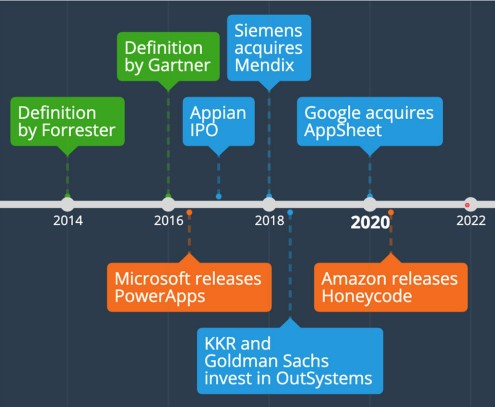
\includegraphics[width=\linewidth]{LCDP_MajorEvents.jpg}
    \caption{Korte historie van low-code development platforms \autocite{Ruscio2022}. Geraadpleegd op 20 maart 2023}
    \label{fig:lcdp_history}
\end{figure}

Een low-code platform wordt door \textcite{Waszkowski2019} omschreven als 'Een set van tools voor programmeurs en niet-programmeurs'. In dit type development platform wordt gesteund op een grafische user interface (GUI) voor het ontwerpen en bouwen van applicaties. Het stelt de gebruiker in staat om snel en met weinig programmeerkennis, een volledige business applicatie op te bouwen. \\

In het algemeen bestaan low-code platformen uit vier lagen. De bovenste laag of Application Layer bevat de GUI waarmee de gebruiker gaan interageren om hun gewenste applicatie op te bouwen. Daarbovenop bevat deze laag de authenticatie en autorisatie mechanismen. De tweede laag of Service Integration Layer maakt verbinding met verschillende diensten aan de hand van API's en authenticatiemechanismen. Vervolgens is er de Data Integration Layer, deze houdt zich bezig met de integratie van gegevens uit verschillende bronnen. Ten slotte is er nog de Deployment Layer die de ontwikkelde applicatie zal opzetten in speciale cloud infrastructuren of on-premise omgevingen, waarbij containerisatie, orkestratie en continue integratie en deployment (CI/CD) gefaciliteerd worden \autocite{Sahay2020}. \\

De ontwikkeling van een applicatie aan de hand van LCDP's verloopt in verschillende stappen. In de eerste fase definiëren gebruikers de concepten en relaties in de applicatie om op die manier het domein te modelleren. Dit gebeurt meestal met behulp van modelleer constructen zoals drag-and-drop die door het platform worden meegeleverd. In de volgende fase, de specificatie van businesslogica, worden de controle- en gegevensstromen van het systeem gedefinieerd zoals grafische workflows. LCDP's voorzien ook interoperabiliteit met externe services en datasources, zodat gebruikers kunnen verbinden en integreren met systemen van derden. Zodra de gewenste applicatie is gespecificeerd en gebouwd, kan het worden gedeployed in een publieke of private omgeving. Vaak gaat deze deployement door in cloud-infrastructuren. De laatste fase is het onderhouden van de applicatie, in de meeste gevallen heeft een low-code development platform features om te reageren op onvoorziene requirements of problemen die kunnen voorkomen terwijl de applicatie online staat \autocite{Ruscio2022}. \\

% \section{Cloud based business management}

\section{Podio}

% TODO Podio (DRAFT) - OK
% TODO Podio (FINAL) - 

\subsection{Ontstaan van Podio}

% TODO Bronnen Toevoegen - OK
Podio werd opgericht in 2009 door Anders Pollas, Jon Froda en Kasper Hulthin \autocite{Crunchbase}. In 2010 werd Tommy Ahler CEO van het bedrijf. Drie jaar na de oprichting, in 2012, werd het bedrijf voor 53 miljoen dollar overgenomen door Citrix, een Amerikaans softwarebedrijf die zich verdiept in virtualisatie, netwerken en Software-as-a-Service (SaaS). \\

\subsection{Wat is Podio?}

% TODO Bronnen Toevoegen - OK
% TODO Wat is Podio? - OK
Podio is een cloud-based collaboration platform dat gebruikers toelaat om op maat gemaakte business software te ontwikkelen. Het kan alle business processen aggregeren in een enkel platform en kan probleemloos uitgebreid worden naar de wensen van de gebruiker. Het voorziet diverse bouwblokken voor het bouwen van mobiele- en desktop applicaties en automatiseringen, zodat het toegepast kan worden in een diverse reeks van use cases. Het doel van Podio is om alle gegevens en communicatie te omvatten in één tool die overal gebruikt kan worden \autocite{Podio}. \\ 

% TODO invoegen figuur Podio Structure https://tallyfy.com/what-is-podio/ - NOK
\begin{figure}
    \centering
    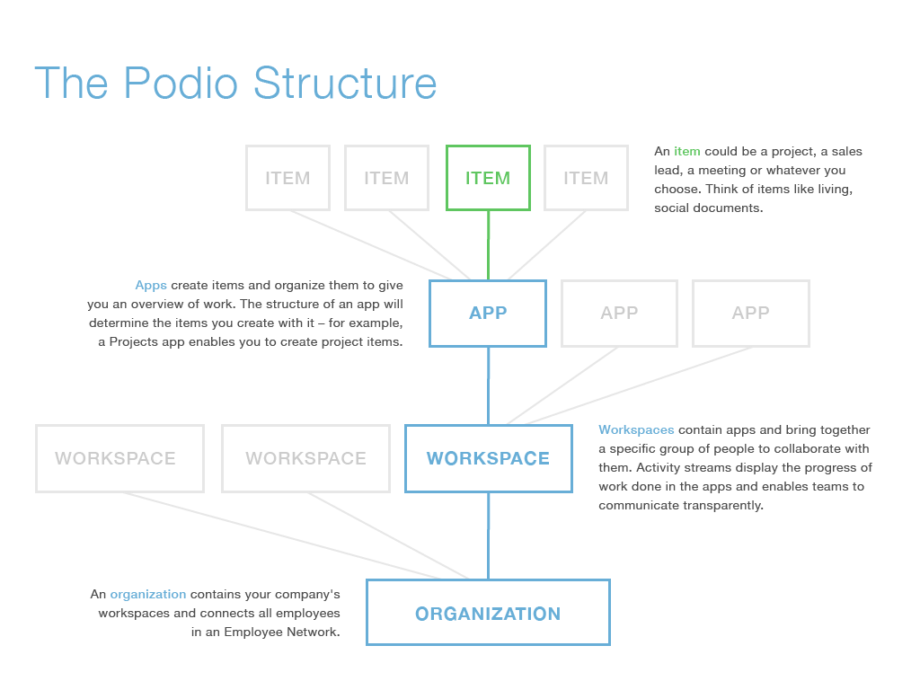
\includegraphics[width=\linewidth]{Podio_Structure.png}
    \caption{Algemene structuur van Podio \autocite{TallyfyPodio}. Geraadpleegd op 24 maart 2023, van https://tallyfy.com/what-is-podio.}
    \label{fig:podio_structure}
\end{figure}

In Podio wordt een organisatie opgedeeld in drie groepen: Workspaces, Apps en Items (zie figuur \ref{fig:podio_structure}). \\

% TODO Workspaces - OK
Het doel van een workspace is om een groep mensen samen te brengen en van relevante apps te voorzien. Elke workspace bevat een activiteiten stroom, op die manier kan ieder groepslid zien wie wat gedaan heeft en wanneer dit gebeurt is \autocite{TallyfyPodio}. Workspaces worden vaak gebruikt om projecten of bedrijven te onderhouden. Er zijn drie types workspaces. Ten eerste is er de open workspace, deze is zichtbaar voor iedereen binnen een organisatie. Ten tweede is er de private workspace, dit type is initieel alleen zichtbaar voor de administrator van de organisatie, andere werknemers kunnen slechts toegang krijgen via een uitnodiging. Ten slotte is er nog de employee workspace, dit speciaal type workspace brengt elk lid van een organisatie samen via hun email domein. Zo heeft bijvoorbeeld iedereen met een @hogent.be email toegang tot de HoGent workspace \autocite{PodioFeatures}. \\

% TODO Apps - OK
% TODO Tabel Features - NOK
Apps creëren meer overzicht binnenin een workspace en helpen het team hun werk op te volgen \autocite{PodioFeatures}. Elke app wordt opgebouwd uit een samenvoeging van bouwblokken of velden, deze staan gelijst in tabel \ref{tab:Tabel 1}. Bovendien heeft Podio ook een app store die bestaat uit pasklare apps, zo kunnen managers een volledig functionele applicatie opzetten in slechts enkele minuten tijd \autocite{TallyfyPodio}. \\

\begin{table}[ht]
    \centering
    \caption{\label{tab:Tabel 1} Lijst met veld types voor Podio apps \autocite{PodioFeatures}.}
    \begin{tabular}{ | p{3cm} | p{11cm} | }
        \hline
        \textbf{Type} & \textbf{Beschrijving} \\
        \hline\hline
        Text & Wordt voor alles gebruikt. \\
        Category & Kan een bepaalde status bevatten en dus gebruikt worden voor filteren of sorteren. \\
        Date & Datum voor projecten of meetings instellen. \\
        Relationship & Wordt gebruikt om verschillende apps aan elkaar te koppelen via gedeelde data. \\
        Contact & Contactpersoon toevoegen aan een item. \\
        Number & Opnemen, rapporteren en berekenen van numerieke waarden. \\
        Link & Delen van links met bijhorende content previews. \\
        Image & Toevoegen van afbeeldingen zoals screenshots of designs. \\
        Money & Opnemen van geldwaarden om budget op te volgen en monetaire berekeningen te maken. \\
        Progress & Simpele progressie visualisatie. \\
        Calculation & Wordt gebruikt voor berekeningen en laat ook JavaScript toe. Dit type veld is een van de belangrijkste en word zeer vaak gebruikt, omdat er hele diverse zaken mee mogelijk zijn. \\
        Map & Locaties opnemen en weergeven via Google Maps. \\
        Duration & Opnemen van een tijdsspanne. \\
        \hline
\end{tabular}
\end{table}
    
% TODO Items - OK
Items worden aangemaakt door apps en kunnen in allerlei vormen voorkomen. Zo zal een project management app bijvoorbeeld projecten als items hebben. In een item wordt de inhoud over één onderwerp opgeslagen, het kan dus in essentie voorgesteld worden als een rij in een database. De manier waarop items gestructureerd zijn, kunnen een grote bijdrage hebben tot je ervaringen met Podio \autocite{TallyfyPodio}. \\

% TODO Quivvy - OK
Quivvy Solutions BV onderzoekt de business processen van hun klanten en welke tools zij daarvoor gebruiken. Hierna gaan ze deze processen gaan configureren in Podio. Daarbovenop onderzoeken ze ook welke tools van de klant gelinkt, of zelfs vervangen kunnen worden door Podio. Verder gaan ze afzonderlijke processen omzetten naar workflows en die, indien mogelijk, ook automatiseren \autocite{QuivvySoftware}. Kortom analyseert Quivvy Solutions de processen en gegevens van hun klanten en zetten deze vervolgens om naar een Podio-omgeving waarmee de klant in staat is om zijn volledige bedrijfsinfrastructuur te beheren. \\

\subsection{Podio API}

% TODO Podio API - OK
% TODO Bronnen Toevoegen - OK

Podio frontend werd volledig gebouwd op zijn Application Programming Interface of kortom API. Hierdoor is het platform gemakkelijk uit te breiden en biedt het tal van mogelijkheden, zo heeft men bijvoorbeeld de mogelijkheid om webhooks te registreren in Podio apps \autocite{PodioAPI2023}. Webhooks zorgen voor dat een bepaalde URL kan aangeroepen worden wanneer een item wordt aangemaakt, aangepast of verwijderd wordt in Podio. Hierdoor kunnen gebruikers event-driven apps bouwen, zoals bijvoorbeeld een notificatie systeem via SMS \autocite{PodioAPIWebhooks}. \\

Momenteel wordt de API voorzien in PHP, .NET, Ruby, Java, Python, Android en Objective-C. Om de API te kunnen gebruiken heeft een gebruiker een API key nodig en moet ze OAuth geauthenticeerd zijn. De Podio API past het RESTful principe toe en gebruikt JSON als zijn uitwisselingsformaat. Vervolgens maakt het gebruik van volgende HTTP methoden om data te manipuleren: GET (ophalen), POST (aanmaken), PUT (bewerken) en DELETE (verwijderen). Bovendien is de API slash-aware, dit betekent dat een URL die eindigt met een schuine streep niet hetzelfde is als een URL zonder het teken. De streep wordt enkel toegevoegd als de bron een lijst van data is \autocite{PodioAPIConcepts}. \\


\subsection{Extensies}

% TODO Bronnen Toevoegen - OK

Het feit dat Podio op zijn API gebouwd is, laat third-party developers toe om hun eigen uitbreidingen of extensies te bouwen op Podio. Deze extensies kunnen heel diverse doeleinden hebben, ze voegen niet alleen extra functionaliteiten toe, maar kunnen ook bestaande processen verbeteren \autocite{PodioExtensions}. Zo is er bijvoorbeeld GlobiMail, die automatisch emails vanuit de inbox neemt en toevoegt als commentaar aan Podio items. Een tweede voorbeeld is SmartGantt, die toelaat om data te visualiseren in Gantt grafieken. Men kan suggesties doen of zelf extensie bouwen en die presenteren aan het Podio team. \\

% https://podio.com/extensions/5
% https://podio.com/extensions/3


\subsection{Workflow Automations (Globiflow)}

% TODO Workflow Automation - OK
% TODO Bronnen aanvullen - OK
Citrix Podio Workflow Automation, vroeger Globiflow genoemd, laat toe om belangrijke taken en processen te automatiseren, om op die manier tijd en geld te besparen. Via triggers kunnen een groot aanbod aan functies uitgevoerd worden op een vastgezet tijdstip of na een bepaalde actie \autocite{PodioWorkflowAutomation}. Elke workflow bestaat uit een trigger, filters en minstens één actie. Triggers kunnen allerlei zaken zijn zoals een bepaald tijdstip, een Podio item die aangemaakt of upgedate wordt, een bepaalde filter, ... \autocite{PodioWorkflowFeatures}. \\

De voornaamste acties die gebruikt worden in workflows zijn;
\begin{itemize}
    \item \textit{Emails of SMS berichten verzenden}: Via deze actie kan men emails of SMS berichten verzenden naar externen. Deze kunnen zelf vooraf opgesteld worden en informatie naar keuze uit Podio items bevatten. Een antwoord op het bericht kan ook gebruikt worden als trigger voor een andere workflow. \autocite{PodioWorkflowFeatures}
    \item \textit{PDF bestanden genereren}: Informatie uit Podio items kan automatisch omgezet worden naar een PDF bestand en indien nodig toegevoegd worden aan emails. Dit kan bijvoorbeeld handig zijn voor het automatiseren van opstellen en verzenden van facturen. \autocite{PodioWorkflowFeatures}
    \item \textit{Embedden in een website}: Door een simpele script tag toe te voegen aan de bron van de website kan data uit Podio items weergegeven worden op de site zelf. Op die manier kan Podio dus gebruikt worden als een eenvoudig Content Management System (CMS). \autocite{PodioWorkflowFeatures}
    \item \textit{Data visualiseren in grafieken}: Een rapport kan via workflows eenvoudig omgezet worden in een grafiek zoals een lijndiagram, taartdiagram, ... Deze grafieken kunnen vervolgens als afbeeldingen weergegeven worden op dashboards in Podio. \autocite{PodioWorkflowFeatures}
    \item \textit{Data feeds}: Soms is het ook belangrijk om data uit Podio te halen en deze te gebruiken in een externe applicatie. Data kan omgezet worden in JSON of XLM en zo doorgegeven worden. \autocite{PodioWorkflowFeatures}
\end{itemize}

\section{Airtable}

% TODO Airtable (DRAFT) - OK
% TODO Airtable (FINAL) - 

\subsection{Ontstaan van Airtable}

% https://builtonair.com/a-brief-history-of-airtable/
% https://nira.com/airtable-history/
% TODO Bronnen Toevoegen - OK

Het idee achter Airtable werd bedacht door Howie Liu in 2012. Hij zag in dat spreadsheets enkel als simpele opslag werden gebruikt, terwijl ze zoveel meer te bieden hadden. Samen met mede-oprichter Andrew Ofstand bouwden ze het idee uit tot een eenvoudig prototype, die ze dan presenteerden aan Amerikaanse acteur Aston Kutcher. Hij besloot direct te investeren, waardoor Airtable officieel gelanceerd werd en begon met development. Twee jaar later, in 2014, starte de open-beta van de app, die toen zeer goed ontvangen werd door de eerste gebruikers. \autocite{Black2019}.
Airtable behoudde dit momentum en bracht in de komende jaren tal van features uit zoals views, integraties en eigen Airtable API \autocite{Shah}. \\

\subsection{Wat is Airtable?}

% TODO Bronnen Toevoegen - OK

Airtable is een low-code/no-code platform waarmee gebruikers op maat gemaakte applicaties kunnen bouwen zonder enige programmeervaardigheden. Het laat toe om eenvoudig een interne database te creëren die belangrijke informatie voor het werk bevat. Bovenop deze database kan dan een krachtige applicatie gebouwd worden die ook workflows en projecten automatiseert. Met Airtable kunnen gebruikers alle informatie met betrekking tot hun doelen en doelstellingen bijhouden en koppelen aan andere tools voor het automatiseren van taken, zoals het verzenden van een email. Automatisaties kunnen getriggerd worden door specifieke acties of tijdstippen. Hierdoor kan men tijd besparen op repetitieve taken en zich focussen op zaken die belangrijker zijn. Daarnaast maakt het platform ook eenvoudige weergave van gegevens mogelijk, via Gantt-grafieken of andere soorten visualisaties. Airtable brengt informatie uit verschillende bronnen samen en stelt gebruikers in staat hun gegevens te sorteren, te filteren en te herschikken om zo aangepaste views (zie \ref{fig:exampleairtable}) voor hun teamleden en partners te creëren. Op die manier heeft iedere stakeholder de informatie die voor hen het meest noodzakelijk is. Het platform biedt gebruikers volledige controle over de applicaties die ze bouwen, ongeacht hun programmeerkennis, dankzij de flexibele en krachtige database die is afgestemd op complexe en specifieke workflows \autocite{AirtableWhat}. \\

% TODO Fig Voorbeeld invoegen https://www.airtable.com/guides/start/what-is-airtable - OK
\begin{figure}
    \centering
    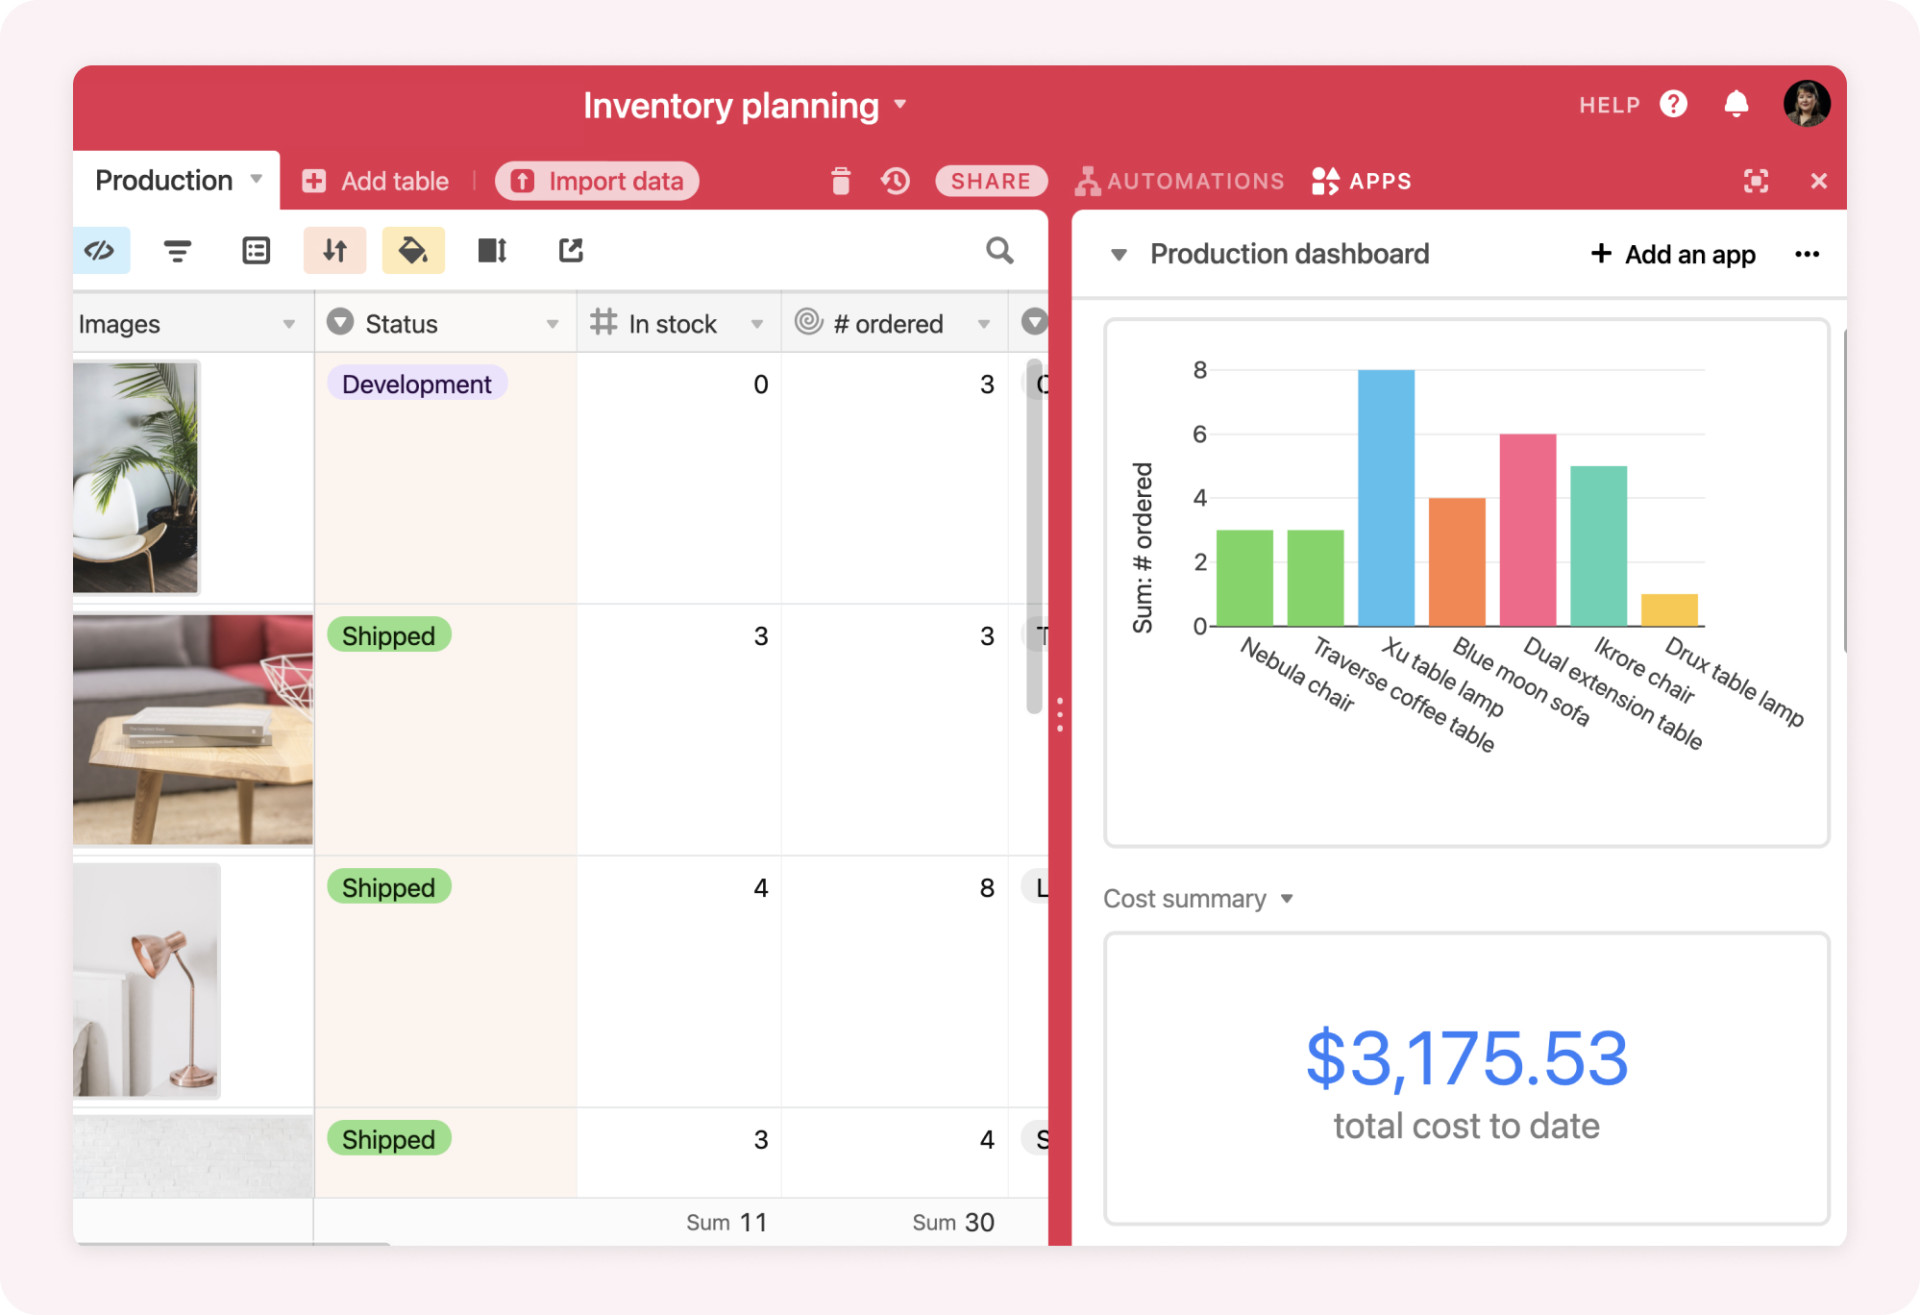
\includegraphics[width=\linewidth]{Airtable_WatIs_Voorbeeld.jpg}
    \caption{Voorbeeld van Airtable view \autocite{AirtableWhat}. Geraadpleegd op 28 maart 2023, van https://www.airtable.com/guides/start/what-is-airtable.}
    \label{fig:exampleairtable}
\end{figure}

Het kernidee van Airtable draait rond het gebruik van een `Single source of truth` of enkele bron van waarheid, die in real-time up-to-date gehouden wordt. Veel processen ondervinden vertragingen 
wanneer men dezelfde informatie meermaals moet gaan bijwerken op verschillende plaatsen. Dit leidt niet alleen tot frustratie, maar soms ook tot fouten, die kunnen resulteren in erge gevolgen. Met Airtable wordt alle data gecentraliseerd en gesynchroniseerd, waardoor het bijwerken van data slechts één keer moet gebeuren. Zo weet elk teamlid dat ze altijd met de meest actuele informatie werken en kunnen eventuele fouten vermeden worden \autocite{AirtableWhat}. \\

\subsection{Airtable Web API}

% TODO Bronnen Toevoegen - OK

Om data te integreren met externe applicaties of systemen wordt gebruik gemaakt van de Airtable Web API. Alhoewel de officiële client gebouwd is in JavaScript, zijn er ook community-built versies beschikbaar in Ruby, .NET, Python 3 en Python 2/3. De API houdt zich aan REST semantiek, gebruikt JSON om objecten te encoderen, en steunt op standaard HTTP codes om resultaten van operaties aan te tonen. \autocite{AirtableAPI} Met deze API kan men data lezen, creëren, updaten en verwijderen. \\

Airtable WEB API maakt gebruik van token-based authenticatie. Dit betekent dat alle requests een persoonlijke of OAuth token in hun header moeten hebben, zoals in figuur \ref{fig:airtable_authtoken} weergegeven \autocite{AirtableAPIAuthentication}. \\

% TODO Fig Auth token invoegen - OK
% TODO Fig Voorbeeld invoegen https://www.airtable.com/guides/start/what-is-airtable - OK
\begin{figure}
    \centering
    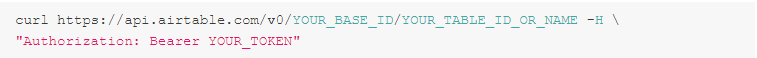
\includegraphics[width=\linewidth]{Airtable_WebAPI_AuthToken.png}
    \caption{Voorbeeld van Airtable API call \autocite{AirtableAPIAuthentication}. Geraadpleegd op 29 maart 2023, van https://airtable.com/developers/web/api/scopes.}
    \label{fig:airtable_authtoken}
\end{figure}

Scopes bepalen welke acties de gebruiker kan uitvoeren en zitten verwerkt in de access token. Er zijn drie verschillende soorten scopes in de Airtable Web API, namelijk `Basic scopes`, `Enterprise member scopes` en `Enterprise admin scope`. Hierbij omvat de `Basic scopes` het minste aantal acties en `Enterprise admin scopes` de meeste. Het is belangrijk om te vermelden dat, om data te bewerken, de gebruiker zowel de juiste scope als toegang tot de data moet hebben. \autocite{AirtableAPIScopes}. Een volledige documentatie van de mogelijke acties kan teruggevonden op de officiële site van Airtable Web API. \\

\section{(Google) AppSheet}

% TODO AppSheet (DRAFT) - OK
% TODO AppSheet (FINAL) - 


\subsection{Wat is AppSheet?}
AppSheet is een no-code development platform dat werd overgenomen door Google in 2020. Het laat toe om mobiele en desktop applicaties te bouwen zonder enige code te hoeven schrijven. Het maakt gebruik van spreadsheets en databases zoals SQL of AWS om automatisch data te visualiseren. Deze weergaven zijn bovendien volledig bewerkbaar door gebruiker zelf \autocite{AppSheet2020}. AppSheet is vooral nuttig voor zakelijke use cases zoals CRM, projectbeheer en gepersonaliseerde rapporten. Het biedt geavanceerde machine learning en AI-functies, waaronder waardevoorspelling, OCR, sentimentanalyse en anomaliedetectie. AppSheet is gratis voor prototyping en persoonlijk gebruik, maar voor commerciële toepassingen is een maandelijks bedrag vereist. Bovendien zijn een actieve internetverbinding en een client app nodig om toegang te krijgen tot AppSheet applicaties en hun functies, aangezien ze in de cloud worden ingezet \autocite{Petrovic2020}. \\

\subsection{AppSheet Templates}

% TODO Bronnen Toevoegen - OK

AppSheet voorziet een groot aanbod aan templates voor verschillende use cases. In tabel \ref{tab:Tabel 2} werden enkele voorbeelden gelijst. 

\begin{table}[ht]
    \centering
    \caption{\label{tab:Tabel 2} Lijst met beschikbare AppSheet templates \autocite{AppSheetTemplates}.}
    \begin{tabular}{ | p{5cm} | p{9cm} | }
        \hline
        \textbf{Template} & \textbf{Beschrijving} \\
        \hline\hline
        Simple Survey & basisstructuur voor formulieren of vragenlijsten aan te maken \\
        Simple Inventory & Bijhouden en monitoren van een opslag \\
        Kanban Board & Projecten en taken opvolgen in een kanban dashboard \\
        Workstation Booking & Reserveren en toewijzen van deelbare ruimtes binnen een organisatie \\
        Order Deliveries & Opvolgen en klanten op de hoogte houden van leveringen \\
        Task Manager & Opvolgen van (herhalende) taken \\
        Facility Assets & Opvolgen van activa binnen een bedrijf \\
        Occupancy Tracker & Opvolgen van de beschikbaarheid van bepaalde kamers of ruimtes \\
        Client Expenses & Opvolgen en sorteren van uitgaven gemaakt door klanten \\
        To Do List & Simpele to do lijst die opgedeeld kan worden in categorieën \\
        Shift Scheduling & Roosteren en onderhouden van shifts voor bedrijfsmedewerkers \\
        Incident Report & Melden en rapporteren van incidenten. \\
        Route Optimization & Routes plannen voor chauffeurs a.d.h.v. Google Maps API \\
        Events Calendar &  Evenementen organiseren op een gedeelde kalender \\
        Contact Manager & Onderhouden en loggen van persoonlijke of business contacten en interacties \\
        \hline
    \end{tabular}
    \vspace{0.3cm}
    {\raggedright \textit{Opm. Deze lijst beperkt zich tot slechts 15 templates} \par}
\end{table}

\subsection{Opzetten van een eenvoudige applicatie in AppSheet}

% TODO Bronnen Toevoegen - OK

Het bouwen van een envoudige applicatie in AppSheet gaat als volgt. Eerst en vooral moet men data voorzien. Het platform ondersteunt verscheidene soorten data bronnen zoals Excel, Cloud SQL, etc. De omschrijving van de data moet in de eerste rij worden geplaatst, op die manier kan AppSheet de data uit elkaar houden. Daarna wordt de data aan de applicatie verbonden, Appsheet host namelijk zelf geen data, maar interageert er enkel mee. Vervolgens moet gedefiniëeerd worden hoe de data gebruikt zal worden, er kan bijvoorbeeld voor gekozen worden om bepaalde data niet weer te geven of om een formule erop toe te passen vooraleer het in de applicatie getoond wordt. Na deze stap word User Interface (UI) opgemaakt, deze bestaat uit views. AppSheet voorziet een hele reeks aan pasklare views die gebruikt en aangepast kunnen worden.  Daarna kan men bots toevoegen om automatisaties te runnen zoals bijvoorbeeld het verzenden van een email. Een bot bestaat uit drie componenten: een event, een taak en een proces. Een event kan gelijkgesteld worden aan een trigger in Podio, het bepaald namelijk wanneer een bot zijn taak moet gaan uitvoeren. Een taak is de actie die moet uitgevoerd worden nadat een event is getriggered. Via een process kunnen verschillende taken opgedeeld worden in stap met eventuele conditionele logica. Ten slotte hoeft men de gemaakte applicatie alleen nog maar te deployen. AppSheet zal nog enkele checks uitvoeren om na te gaan of de app proper werkt en vervolgens live zetten. De applicatie kan dan gedownload worden of geopend worden in een web browser \autocite{AppSheetHowToCreate}. \\

%%=============================================================================
%% Methodologie
%%=============================================================================

\chapter{\IfLanguageName{dutch}{Methodologie}{Methodology}}%
\label{ch:methodologie}

%% OK - In orde
%% BOK - Bijna in orde
%% NOK - Niet in orde

%% TODO: Hoe ben je te werk gegaan? Verdeel je onderzoek in grote fasen, en
%% licht in elke fase toe welke stappen je gevolgd hebt. Verantwoord waarom je
%% op deze manier te werk gegaan bent. Je moet kunnen aantonen dat je de best
%% mogelijke manier toegepast hebt om een antwoord te vinden op de
%% onderzoeksvraag.

% TODO - Inleiding - OK
In dit hoofdstuk wordt de Methodologie van het onderzoek beschreven en uitgelegd. Dit is deels een vervolgstuk op de technologieën die in de literatuurstudie besproken werden. Eerst en vooral komt een requirements-analyse en vooronderzoek aan bod, waaruit de potentiële kandidaten voor het onderzoek bekomen worden. In het vooronderzoek wordt een long list opgesteld waarvan. \\

Omdat Quivvy Solutions het belangrijk vindt up-to-date te blijven over diverse low-code platformen, hebben ze zelf reeds onderzoek gedaan naar een potentieel alternatief. Om die redenen is een van de kandidaten, Airtable, reeds gekozen uit de long list van kandidaten. Dit is één van de platformen waar het bedrijf veel interesse in heeft en graag zou laten onderzoeken. Desondanks het feit dat het reeds geselecteerd is, zal in het vooronderzoek de verschillende vereisten voor Airtable toch nog overlopen worden. \\


\subsection{Requirements-analyse}

De requirements voor een goed alternatief werden opgesteld aan de hand van de noden van Quivvy Solutions. Zij ontwikkelen low-code oplossingen voor kleine tot middelgrote bedrijven en gebruiken daarvoor voornamelijk Podio. De platformen moeten dus op zijn minst over de basisfunctionaliteiten van Podio beschikken. Bovendien moet er ook nagegaan worden of de alternatieven een goede toekomst hebben. Uiteindelijk werden de nodige vereisten verder opgedeeld in functionele en niet-functionele vereisten. \\

\textbf{Functionele vereisten:} % TODO FR - OK

\begin{itemize}
    \item De datastructuur moet bestaan uit een enkele database die zich als\textbf{`Single source of truth}` voordoet. Met andere woorden, het platform moet voor een applicatie een enkele database voorzien zodat alle data slechts op één plek wordt opgeslagen.
    \item Het platform moet over een bepaald minimum aan \textbf{flexibiliteit} bezitten. Dit betekent het zich niet mag focussen op specifieke use cases, maar dat het gebruikt kan worden voor elke context. Indien iets toch niet mogelijk is, moeten er workarounds of extensies aanwezig zijn die dit probleem verhelpen.
    \item Het platform moet in staat zijn om zaken zoals \textbf{workflows te automatiseren}.
    \item Het platform moet over een \textbf{eigen AP}I bezitten.
\end{itemize}

\textbf{Niet-functionele vereisten:} % TODO NFR - OK

\begin{itemize}
    \item Het platform moet \textbf{low-code/no-code} zijn.
    \item Het platform moet een stevige \textbf{gebruikersbasis} hebben. Dit betekent dat het minstens door ongeveer 250.000 gebruikers en 3000 bedrijven in gebruik moet zijn.
    \item Het platform moet \textbf{stabiel} zijn. Dit betekent dat het geen frequente storingen ondervindt en dat het zich beperkt tot maximaal twee incidenten per maand.
    \item Het platform moet \textbf{futureproof} zijn. Dit betekent dat het platform zeer sterk aan het groeien moet zijn. Hierbij wordt gekeken naar het aantal werknemers, de winst en de opgehaalde financiering op jaarbasis.
\end{itemize}


\subsection{Long list}
% - Tabel   nocode/ lowcode LONG LIST
\begin{table}[ht]
    \centering
    % TODO Add bron: https://analyticsindiamag.com/10-low-code-no-code-platforms-every-developer-should-know-of/ OK
    \caption{\label{tab:Tabel 3} Lijst met Podio alternatieven die onderzocht kunnen worden \autocite{Tasmia2022}.}
    \begin{tabular}{ | p{5cm} | p{2cm} | p{2cm} | }
        \hline
        \textbf{Platform}   & \textbf{Low-code} & \textbf{No-Code} \\
        \hline\hline
        Airtable            & ✓ & ✓ \\
        Appian              & ✓ & ✓ \\
        GoogleAppSheet      &    & ✓ \\
        Mendix              & ✓ & ✓ \\
        Notion              &    & ✓ \\
        Nintex              & ✓ & ✓ \\
        Shopify             & ✓ & ✓ \\
        Visual LANSA        & ✓ &    \\
        Kissflow            & ✓ &    \\
        Quixy               &    & ✓ \\
        ZohoCreator         & ✓ &    \\
        Caspio              &    & ✓ \\
        \hline
    \end{tabular}
    
    {\raggedright \textit{Opm. Er zijn nog alternatieven die niet in deze lijst vermeld staan.} \par}
\end{table}

\subsection{Short list}

Uit de long list werden Airtable en Google AppSheet gekozen, deze twee vormen samen de Short List voor het onderzoek. In de volgende 2 secties wordt de keuze voor deze kandidaten onderbouwd. 

\subsection{Airtable} % TODO - Airtable - BOK


% Low-code / Flexibel
Airtable is low-code en voorziet voorgemaakte templates voor tal van diverse use cases, zoals een `Product Catalog` of een `Customer Relationship Management (CRM)`. Daarnaast heeft de gebruiker natuurlijk ook de mogelijkheid om zelf een applicatie op te bouwen. Om die redenen kan het dus zeker als een flexibel platform beschouwd worden. \\
% TODO - https://www.softr.io/airtable/airtable-use-cases

% API / Automations
Zoals in de sectie \ref{subsec:airtable_web_API} werd vermeld, bevat Airtable ook een krachtige API die het verkrijgen, aanmaken, updaten en verwijderen van een of meerdere records voorziet. Vervolgens zijn ook automatisaties mogelijk met Airtable. Via triggers kan men verschillende soorten actions automatisch laten uitvoeren. \\
% TODO - https://airtable.com/developers/web/api/introduction (al aanwezig in bibtex)
% TODO - https://support.airtable.com/docs/getting-started-with-airtable-automations

% Futureproof
Toen het bedrijf in 2013 begon, had het minder dan 10 werknemers en was er slechts 3 miljoen dollar aan financiering beschikbaar. Maar tegen het einde van 2021 had Airtable aanzienlijke vooruitgang geboekt: het beschikte op dat moment ongeveer over 700 werknemers en wist maar liefst één miljard dollar aan financiering op te halen. Dit is een enorme verbetering ten opzichte van het voorgaande jaar, waarin slechts 185 miljoen dollar werd opgehaald. Bovendien werd in 2021 de waarde van Airtable geschat op 11,7 miljard dollar, wat ongeveer 5 miljard meer is dan in 2020. Ten slotte is de jaarlijkse groei van het bedrijf is ongeveer 39\% en brengt het maandelijks meerdere updates uit. Uit voorgaande informatie kan dus besloten worden dat het platform zeker futureproof is. \\
% TODO - https://www.mksguide.com/airtable-user-and-company-stats/
% TODO - Invoegen Airtable_Valuation_2018_To_2021.png

% Stabiel
Airtable heeft de afgelopen 2 jaar (januari 2021 tot december 2022) gemiddeld 1 à 2 incidenten per maand gehad, deze incidenten werden meestal ook de dag zelf nog opgelost . Het voldoet dus aan de vastgelegde requirement. \\
% TODO - https://status.airtable.com/history

% Gebruikersbasis
Airtable wordt gebruikt door meer dan 300.000 bedrijven, waaronder Shopify, Nike en AT\&T. Bovendien gebruikt 80\% van de `Fortune 100`\footnote{Groep met de 100 grootste bedrijven van de Verenigde Staten} het platform. Vervolgens heeft meer dan 30\% van de klanten zich ingeschreven voor een betaald plan. \\
% TODO - https://nira.com/companies-that-use-airtable/


\subsection{AppSheet} % TODO - keuze AppSheet - NOK

% Low-code / Flexibel
De tweede kandidaat voor het onderzoek is het no-code platform Google AppSheet. Het voorziet een groot aantal voorgemaakte templates of 'sample apps' die voor verschillende use cases gebruikt kunnen worden. Alhoewel het platform in het algemeen minder flexibel is dan Podio of Airtable, voldoet het wel aan de requirement. Verder heeft het platform ook een eigen API, maar deze is iets minder uitgebreid dan diegene van Airtable of Podio \\

Daarnaast wordt het platform vaak gebruikt door organisaties met meer dan 10.000 werknemers. Meta Platforms, Inc.\footnote{https://www.meta.com/} of kortweg Meta, het Amerikaans moederbedrijf van ondere andere facebook, is maakt bijvoorbeeld gebruik van AppSheet. Verder is het platform geïntegreerd met Google Workspace en wordt ervan verwacht dat het blijft groeien. Bovendien heeft Google Workspace in 2022 aangekondigd dat ze van plan zijn om te investeren in cursussen en opleidingen voor AppSheet. Uit voorgaande informatie kan dus besloten worden dat AppSheet ook een futureproof platform is. \\ 

Vervolgens kan er besloten worden dat AppSheet voldoet aan de stabiliteits-requirement. Sinds begin 2023 heeft het platform nog maar één keer down time gehad, namelijk in januari 2023. \\
%TODO - https://www.saashub.com/appsheet-status

Ten slotte zijn ook tal van automatisaties mogelijk via AppSheet, die in het platform 'bots' genoemd worden. \\
%TODO - https://workspace.google.com/blog/product-announcements/hidden-secret-open-secret-year-ahead-appsheet



\section{De uit te bouwen Use Case} % TODO - OK

Als use case werd in samenspraak met Quivvy Solutions gekozen voor een eenvoudige applicatie die een simpel stageproces bijhoudt. Ten eerste moet er dus een lijst met studenten en hun gegevens bijhouden worden. Bovendien moet elke student gelinkt zijn aan een dossier, waar verschillende zaken aan vast hangen zoals onder andere een toegewezen begeleider, sollicitaties die de student gedaan heeft, evaluaties gegeven door een begeleider, een toegewezen stageopdracht en een totaal score voor het dossier. Hieruit volgt dus dat er ook andere lijsten zoals docenten, sollicitaties,$\ldots$ aanwezig moeten zijn binnen de applicatie. Daarnaast heeft een student ook een richting die dan op zich meerdere specialisaties bevat, dit zijn ook elementen die als lijst moeten worden opgeslagen. Vervolgens moet er ook de mogelijkheid zijn om het dossier eenvoudig om te vormen naar een PDF bestand. Hiermee is het concept van de use case toegelicht, een verdere uitwerking volgt in de analyse fase van het onderzoek. \\

\newpage

\section{Onderzoek} 
In deze sectie wordt het effectieve onderzoek besproken, waarbij wordt beschreven hoe de use case is ontwikkeld op verschillende platformen en in hoeverre dit voldeed aan een reeks criteria. De criteria voor het onderzoek zijn als volgt geformuleerd;

\begin{itemize}
    \item Hoe eenvoudig is het om \textbf{relaties} te leggen tussen verschillende onderdelen, bijvoorbeeld tussen een studierichting en zijn specialisaties?
    \item Is het mogelijk om een studentendossier \textbf{automatisch om te vormen} naar een PDF met de nodige informatie? Indien wel, hoe gemakkelijk lukt dit?
    \item Is het mogelijk om via \textbf{workflows} sollicitaties/stageopdrachten aan te maken en deze automatisch te linken met de overeenkomstige student/bedrijf?
    \item Hoe eenvoudig is het om \textbf{calculaties} of berekeningen uit te voeren, zoals een overzicht opstellen van de verschillende stageopdrachten die een bedrijf voorziet?
    \item Hoe aangenaam is de \textbf{gebruikerservaring}? Met name hoeveel keer moet men klikken of navigeren om een bepaald doel te bereiken? Is de tool eenvoudig te gebruiken of is de bediening eerder complex?
    \item Hoe intuïtief is de \textbf{user interface (UI)}? Is deze overzichtelijk of staan er veel zaken door elkaar? Hoe eenvoudig kan een bepaalde functie terug gevonden? Kunnen activiteiten gemakkelijk opgevolgd worden, bijvoorbeeld via dynamische views of tegels?
    \item Hoe \textbf{probleemloos} verloopt het uitbouwen van de use case? Welke problemen komt men allemaal tegen?
\end{itemize}

\subsection{Analyse Use Case}

Net zoals bij andere IT projecten is het belangrijk om eerst een analyse uit te voeren voordat er effectief gestart wordt met ontwikkelen. De analyse voor een use case kan verschillen afhangend van het platform waarvoor men ze wil uitvoeren. Aangezien deze studie alternatieven zoekt voor Podio, wordt de analyse fase uitgevoerd in functie van Podio en daarna toegepast op Airtable en Google AppSheet. \\

In Podio wordt een database tabel voorgesteld als een app, die informatie over een bepaald onderwerp bijhoudt. Uit de beschrijving van de use case kan afgeleid worden er op zijn minst 9 apps aanwezig moeten zijn, namelijk studenten, bedrijven, docenten, stageopdrachten, sollicitaties, richtingen, specialisaties, studentendossiers en evaluaties. \\

Het is belangrijk om in te zien dat studenten en docenten beide personen zijn en dat een bedrijf ook meerdere contactpersonen kan hebben. Om een persistente structuur te hebben, is er dus een 10de app genaamd ‘Contacten’ nodig. Bovendien voorkomt dit ook eventuele redundante data. Een docent kan bijvoorbeeld contactpersoon zijn bij een bedrijf, maar dit kan moeilijk aangetoond worden, aangezien er geen expliciete relatie is tussen ‘Bedrijven’ en ‘Docenten’. Deze persoon zou dus twee keer moeten opgeslagen worden in de databank, wat tegenin de richtlijnen van Podio gaat. \\

Daarnaast moet er ook rekening gehouden worden met het leggen van relaties tussen de verschillende apps. In Podio is het bij het 1-op-1 relaties en 1-op-veel relaties beter om de relatie bij slechts één van de twee te apps leggen en bij de andere een calculatie veld te gebruiken. Anders kan er verwarring ontstaan binnenin het platform, indien er bijvoorbeeld een item verwijderd wordt kan de relatie aan één van de kanten nog steeds bestaan. \\

Tenslotte is het belangrijk om na te denken welke automatisaties allemaal toegepast kunnen worden. In dit onderzoek wordt er beperkt tot de volgende;

\begin{itemize}
    \item Automatisch aanmaken van een sollicitatie en linken aan een dossier.
    \item Automatisch aanmaken van een evaluatie en linken een dossier.
    \item Automatisch aanmaken van een stageopdracht en linken aan een bedrijf.
    \item Automatisch invullen van richting wanneer een specialisatie wordt gelinkt aan een stageopdracht.
    \item Automatisch aanmaken van een specialisatie en linken aan een richting.
    \item Dossier automatisch omvormen tot een opgemaakt pdf-bestand.
\end{itemize}

\begin{table}
    \centering
    \caption{\label{tab:Resultaat analyse} }
    \begin{tabular}{ | p{4cm} | p{8cm} | }
        \hline
        \textbf{App} & \textbf{Attributen} \\
        \hline\hline
        Contacten       & (calc.\footnote{calculatie}) ID, voornaam, familienaam, adres, geboortedatum, email, telefoonnummer, (calc.) Bedrijven \\
        Studenten       & (calc.) ID, (rel.\footnote{relatie}) Contact, (rel.) Studierichting, (rel.)  Specialisatie, klasgroep \\
        Bedrijven       & (calc.) ID, naam, adres, email, telefoonnummer, link, (rel.) Contactpersonen, (calc.) Stageopdrachten \\
        Docenten        & (calc.) ID, rol, (rel.) Studierichting \\
        Stageopdrachten & (calc.) ID, titel, (rel.) Bedrijf, beschrijving, (rel.) Richting, (rel.) Specialisaties, periode, aantal-studenten, (rel.) Toegewezen-aan \\
        Sollicitaties   & (calc.) ID, (rel.) Student, (rel.) Bedrijf, datum-gesprek, alleen/medestudent, (rel.) Medestudent, resultaat, opmerking \\
        Richtingen      & (calc.) ID, naam, afkorting, status, (calc.) Specialisaties \\
        Specialisaties  & (calc.) ID, naam-specialisatie, (rel.) Richting \\
        Dossiers        & (calc.) ID, Titel, (rel.) Student, (rel.) Begeleider, (rel.) Sollicitaties, (rel.) Evaluaties, (rel.) Toegewezen-stageopdracht, (calc.) Score \\
        Evaluaties      & (calc.) ID, datum, (rel.) Student. \\
        \hline
    \end{tabular}
\end{table}

Nu de analyse fase voltooid is kan er gestart worden met het ontwikkelen in Podio, Airtable en Google AppSheet. Vervolgens wordt voor elk van de platformen nogmaals de criteria overlopen en wordt er toegelicht hoe goed elk platform eraan voldoet. \\

\newpage



% PODIO __________________________________________________________________________________________________________________________
\subsection{Podio} % TODO - Podio - OK

Vooraleer het bouwproces wordt toegelicht is het belangrijk om nog eens de structuur van Podio op te frissen. In Podio wordt een use case of project weergegeven aan de hand van een workspace. Deze workspace bevat één of meerdere apps die een template voorzien voor een bepaald onderdeel. Een template wordt gebruikt om een item van de app op te bouwen en is een samenstelling van velden zoals een tekstveld, datumveld of calculatieveld. Vanuit een database-perspectief kan een workspace dus gezien worden als de database, een app als een tabel, een template als de kolommen van de tabel en een item als een rij in een tabel. \\

In Podio is de eerste stap van het ontwikkelingsproces dus het aanmaken van de workspace waarin alles gebouwd zal worden. De ‘Activity’ app, zie figuur \ref{fig:meth_podio_workspace}, wordt standaard aangemaakt bij het creëren van een workspace en bevat een overzicht van wat er zich allemaal afspeelt. Indien iets wordt aangepast, wordt dit weergegeven in een tijdslijn samen met de persoon die het heeft aangepast en wanneer de aanpassing verricht werd. Daarnaast wordt ook een kalendertegel en een lijsttegel, met taken die zelf toegevoegd kunnen worden, voorzien. Bovendien is er de optie om zelf tegels toe te voegen die data uit de workspace kunnen weergeven. \\

\begin{figure}[ht]
    \centering
    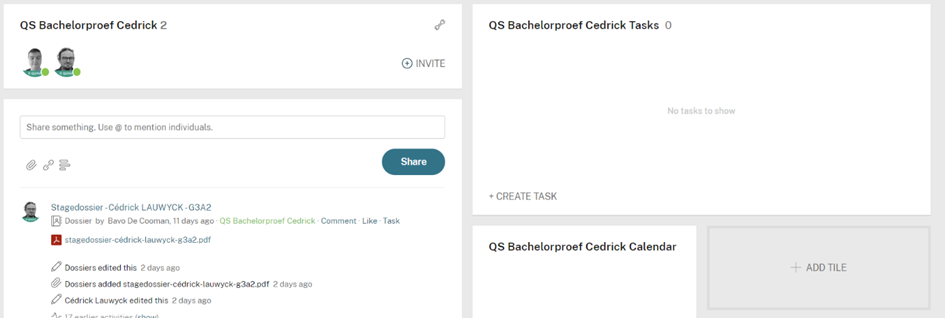
\includegraphics[width=\linewidth]{methodologie/Podio_workspace.png}
    \caption{'Activity' app in een Podio workspace.}
    \label{fig:meth_podio_workspace}
\end{figure}

Nadat de workspace is aangemaakt, kan voor elk onderwerp uit de analyse een app aangemaakt worden. Het is voordeliger om eerste alle apps aan te maken vooraleer de attributen worden toegevoegd, want men kan namelijk geen relatie leggen naar iets dat nog niet bestaat. Dit kan eenvoudig gedaan worden door op de ‘Add App’-knop te klikken, waarna een venster getoond wordt die vraagt achter de naam van de app, de naam van een item en icoon. Voor de benamingen wordt door Quivvy vaak enkelvoud en meervoud gebruikt, ter illustratie: de ‘Contacten’ app heeft ‘Contact’ als naam van het item. Het icoon daarentegen kan gekozen worden uit een uitgebreide lijst van iconen. Het uiteindelijke resultaat van deze stap wordt weergegeven in figuur \ref{fig:meth_podio_lijstApps}. \\

\begin{figure}[ht]
    \centering
    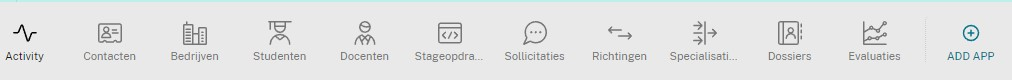
\includegraphics[width=\linewidth]{methodologie/Podio_lijstApps.jpg}
    \caption{Aangemaakte apps in de Podio workspace.}
    \label{fig:meth_podio_lijstApps}
\end{figure}

Eens alle apps aangemaakt zijn, is de fundering van de use case afgewerkt. Nu kan er over gegaan worden tot het instellen van de verschillende attributen en relaties. Dit is mogelijk in 2 simpele klikken, namelijk door naar de app te navigeren en vervolgens via het ‘moersleutel’-icoontje de verschillende instellingen van de openen. Daarna kan men via een derde klik de template van de app gaan bewerken. Zoals eerder vermeld is een template een samenstelling van verschillende types velden die Podio voorziet. Voor de use case wordt dus elk voor elk attribuut van de app een veld toegevoegd. Ter illustratie wordt in figuur \ref{fig:meth_podio_dossierTemplate} de uitgewerkte template voor de 'Dossiers' app van de use case weergegeven. Eerst een vooral werd een calculatieveld toegevoegd voor de ID van het dossier. In dit veld komt het low-code gedeelte van Podio aan bod, het veld accepteert namelijk JavaScript en kan op allerlei manieren gebruikt worden. De laatste lijn in het calculatie veld is wat er uiteindelijk wordt weergegeven, daaronder is ook een preview zichtbaar. In het geval van een dossier wordt een stuk tekst samengevoegd met de ID van de student. Vervolgens wordt een simpel tekstveld gebruikt voor de titel van het dossier, gevolgd door 2 relatievelden om de student en begeleider te linken. Daarna wordt een categorieveld ingevoegd met de opties `Evaluatie` en `Sollicitatie`, dit zal later gebruikt worden voor het toevoegen van een evaluatie of sollicitatie via automatisaties. Podio voorziet namelijk geen knop velden, om die reden wordt een categorie veld gebruikt als workaround. Verder worden nog 2 relatievelden toegevoegd en nog een calculatieveld waarin de totaalscore van de evaluaties wordt uitgerekend en weergegeven. Het is belangrijk om te vermelden dat er voor elk een set van opties beschikbaar zijn, om bijvoorbeeld het veld verplicht te maken of om het aantal relaties in een relatieveld te beperken. \\

\begin{figure}[ht]
    \centering
    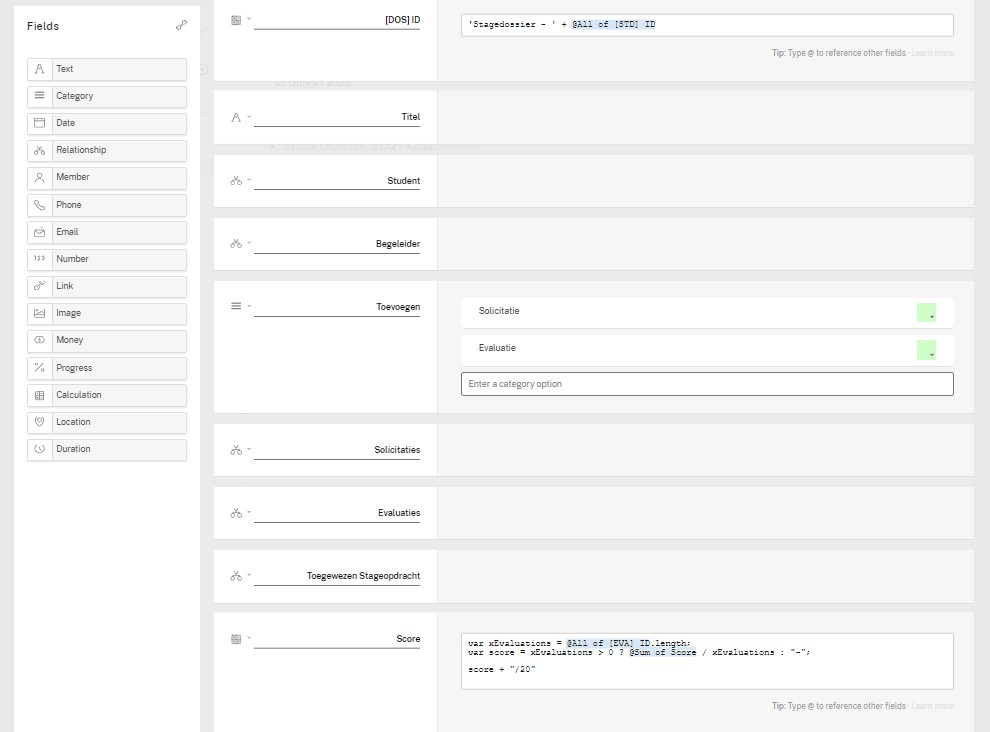
\includegraphics[width=\linewidth]{methodologie/Podio_dossierTemplate.jpg}
    \caption{Uitgewerkte template van de 'Dossier' app.}
    \label{fig:meth_podio_dossierTemplate}
\end{figure}

Om de data mooi weer te geven wordt als extra ook de layout aangepast. Podio voorziet standaard 5 verschillende layouts, namelijk 'Badge', 'Table', 'Card', 'Activity' en 'Calender', verder kunnen ook nog filters ingesteld worden op de attributen van een app. Eens alles geconfigureerd is naar keuze kan ten slotte de weergave als view worden opgeslagen. In figuur \ref{fig:meth_podio_badgeLayout} is een voorbeeld van de badge layout te zien. Bovendien kan men voor elke app via de 'Layout options' selecteren welke velden men wil weergeven op een individuele badge. \\

\begin{figure}[ht]
    \centering
    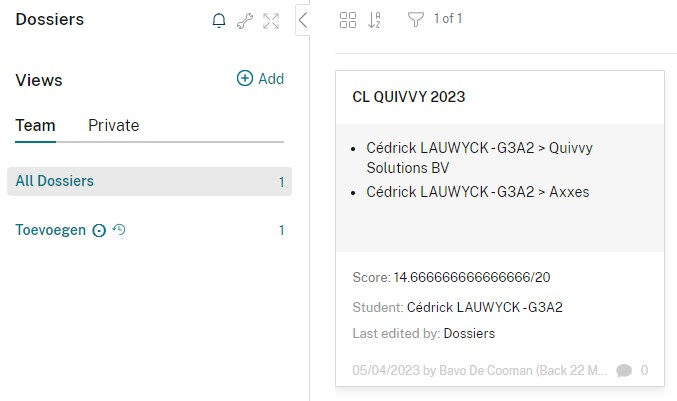
\includegraphics[width=\linewidth]{methodologie/Podio_badgeLayout.jpg}
    \caption{Badge layout in Podio.}
    \label{fig:meth_podio_badgeLayout}
\end{figure}

De volgende stap is om de automatisaties of workflows toe te voegen, dit gebeurt via Globiflow\footnote{wordt ook wel Citrix Podio Workflow Automation genoemd.}, een geavanceerde workflow automation tool gemaakt voor Podio. Door naar de instellingen van een willekeurige app te navigeren en vervolgens door te klikken op `workflow automations`, wordt men omgeleid naar een externe pagina waar automatisaties kunnen worden ingesteld. Eerst en vooral is het belangrijk om onderaan de pagina op de 'Refresh from Podio' knop te klikken, deze zorgt er namelijk voor dat de laatst opgeslagen configuratie van de Podio workspace wordt opgehaald. Nu alle apps en bijkomende velden aanwezig zijn, kunnen er workflows aangemaakt worden. Deze bevatten een trigger, een set van filters en een set van acties die worden uitgevoerd. Er zal dus voor elke automatisatie in de analyse, een workflow aangemaakt worden. Een handige feature van Globiflow, is dat het voor elke workflow ook een verkorte versie of recept weergeeft. Bovendien wordt ook een schatting weergegeven van hoeveel minuten er bespaard worden door de workflow uit te voeren. \\

In figuur \ref{fig:meth_podio_workflow} is terug een uitgewerkt voorbeeld te zien, namelijk het omvormen van een dossier tot pdf bestand. De trigger voor deze workflow is het updaten van een dossier, in de filters wordt dit dan verfijnd tot het updaten van het 'verwerken' veld. Eens dit op `Omzetten naar PDF` wordt gezet, zal de flow verdergaan naar de acties, bij een andere waarde wordt de flow beëindigt. Bij de eerste actie wordt een variabele opgeslagen met het jaartal van creatiedatum van het dossier, deze zal dan later gebruikt worden in de template voor het omvormen naar PDF. Vervolgens wordt de data van enkele referenties opgehaald, namelijk de informatie over de student, studierichting en het bedrijf. Daarna komt het omzetten naar PDF bestand, men kan volledig zelf een template opbouwen met alle nodige informatie uit Podio. Bovendien is het ook mogelijk om een footer en header in te stellen, voor onze use case wordt in de footer bijvoorbeeld informatie over Hogeschool Gent weergegeven. Er hoeft geen actie toegevoegd te worden om de gemaakte PDF aan het item zelf te hangen, want dit zit namelijk inbegrepen in de actie. Indien men het bestand zou willen doormailen kan dat eenvoudig door vanuit deze workflow een andere workflow te activeren en vervolgens de PDF mee te geven. De voorlaatste stap van automatisatie is het `Dossier` item terug updaten om het 'Toevoegen' veld terug op leeg te zetten. Ten slotte worden nog enkele acties toegevoegd om de referenties die eerder werden opgehaald terug op te ruimen, eens dit gebeurt is, is de workflow afgewerkt. \\

\begin{figure}[ht]
    \centering
    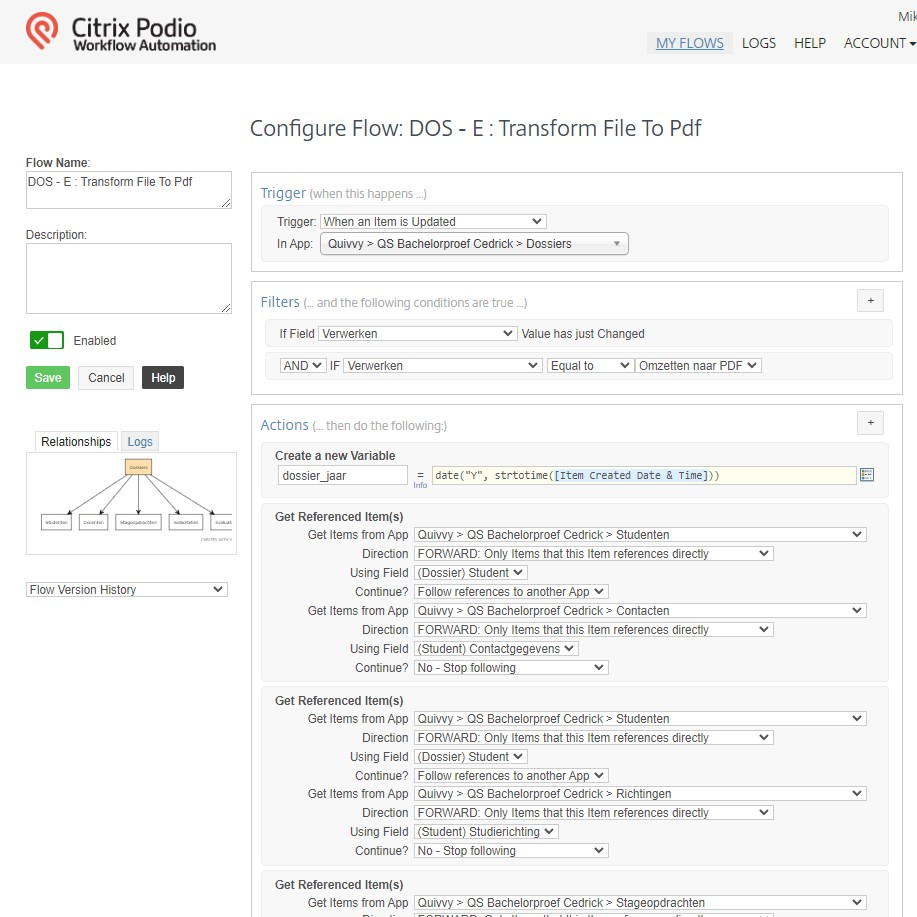
\includegraphics[width=\linewidth]{methodologie/Podio_workflow.jpg}
    \caption{Workflow in Globiflow.}
    \label{fig:meth_podio_workflow}
\end{figure}

Nu de use case is voltooid in Podio, is het belangrijk om de criteria eens door te nemen en kort te evalueren hoe goed het platform presteert. Allereerst is het heel eenvoudig om relaties te leggen via het relatieveld, hoewel er wel altijd nagedacht moet worden aan welke kant de relatie wordt gelegd. Ten tweede kunnen workflows ook gemakkelijk worden ingesteld. Alles heeft een duidelijke benaming, waardoor zelfs lange reeksen van acties eenvoudig te begrijpen zijn. Bovendien biedt Podio een zeer prettige gebruikerservaring. De verschillende knoppen en functies zijn gemakkelijk te begrijpen en kunnen met slechts 1 tot 4 klikken worden bereikt. \\

Het uitbouwen van de use case is echter niet zonder problemen verlopen. Bijvoorbeeld, het instellen van de 'layout options' voor een badge moest vaak twee keer worden toegepast, omdat ze de eerste keer niet werden opgeslagen in het systeem. \\

\newpage



% AIRTABLE __________________________________________________________________________________________________________________________
\subsection{Airtable} % TODO - Airtable - OK

Nu de use case uitgewerkt is in Podio kan overgegaan worden naar het eerste potentiële alternatief, Airtable. De structuur van Airtable is gelijkaardig aan die van Podio, ook hier wordt weer gewerkt met workspaces. In een workspace kan dan een base of database worden aangemaakt, deze zal alle data van de use case omvatten. Verder bestaat een base uit zogenaamde `Tables` of tabellen, die vergelijkbaar zijn met apps uit Podio of dus met een tabel in een database. Voor elk onderwerp uit de analyse wordt dus een tabel toegevoegd, de attributen of kolommen zullen later ingesteld worden. Bij het aanmaken wordt er gekozen om een lege tabel aan te creëren. Daarnaast voorziet Airtable net zoals Podio ook de optie om een tabel aan te maken gebaseerd op een csv-bestand\footnote{simpel bestandsformaat om tabulaire data op te slaan}. Daarnaast kan er ook data uit verschillende andere bronnen zoals Google Drive, Salesforce of Jira Server,$\ldots$ Wat niet standaard ingebouwd zit in Podio. \\

Wanneer alle tabellen aangemaakt zijn, ziet de structuur eruit zoals in figuur \ref{fig:meth_airtable_tables}. Airtable maakt gebruik van een tabblad structuur, waardoor er geen nieuwe pagina moet worden ingeladen om te wisselen van tabel, dit zorgt dan weer voor een zeer aangename gebruikerservaring. \\

\begin{figure}[ht]
    \centering
    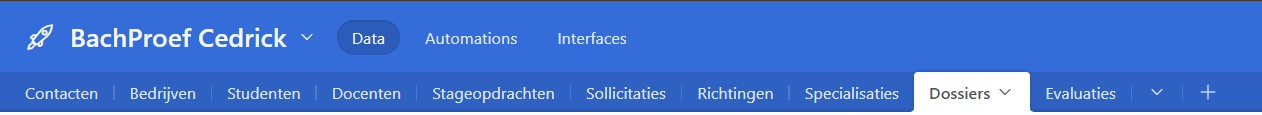
\includegraphics[width=\linewidth]{methodologie/Airtable_tables.jpg}
    \caption{Tables in Airtable.}
    \label{fig:meth_airtable_tables}
\end{figure}

Eens de vorige stap voltooid is, kunnen de attributen per tabel worden ingesteld. In Airtable stelt elke kolom van een tabel een attribuut voor. Om die redenen zijn er dus ook verschillende soorten velden, zoals een `Email` veld om e-mail bij te houden of een 'Phone' veld om een telefoonnummer bij te houden. Een klein verschil met Podio is dat Airtable geen speciaal veld om een adres op te slaan voorziet. Dit is toch wel belangrijk en maakt het bijhouden van een adres minder eenvoudig, aangezien dit dus door een gewoon tekstveld moet gebeuren. \\

De twee belangrijkste types velden zijn het `Relationship` veld en het `Formula` veld. Zoals de naam impliceert, wordt het `Relationship` veld gebruikt om, net zoals in Podio, relaties te leggen tussen de verschillende tabellen. Relaties op zich zijn goed uitgewerkt in Airtable, in tegenstelling tot Podio worden ze direct aan beide kanten toegevoegd. Dit betekent dat als er bijvoorbeeld in de `Specialisaties` tabel een link gelegd wordt naar `Richtingen`, dan zal er ook automatisch een veld worden toegevoegd in de tabel van 'Richtingen'. Bovendien kan er net zoals in Podio gekozen worden of het veld één of meerdere referenties mag bevatten. Verder heeft Airtable ook nog het `Lookup` veld, waarmee een waarde uit een andere tabel kan worden weergegeven. Om dit in Podio te bereiken zou een calculatie veld gebruikt moeten worden. \\

Het 'Formula' veld is vergelijkbaar met een calculatieveld in Podio. Hiermee kunnen aangepaste formules gemaakt worden op basis van andere velden in dezelfde table. Bovendien ondersteunt het veld een groot aantal functies en operatoren, waaronder wiskundige, logische en tekstfuncties. Verder is ook conditionele logica zoals een 'if-else' structuur mogelijk binnen dit veld. Kortom is het dus een krachtig hulpmiddel voor gegevensverwerking binnen Airtable.  In de use case wordt dit type veld vooral gebruikt om de ID's van de verschillende tabellen te berekenen. \\
 
In figuur \ref{fig:meth_airtable_dossiersTable} is de uitgewerkte tabel voor de 'Dossiers' weergegeven, waarvan structuur van de opzet is nagenoeg dezelfde als die in Podio, op enkele verschillen na. Zo wordt voor de totaal score bijvoorbeeld gebruik gemaakt van een ander soort veld dan het `Formula` veld. In tegenstelling tot Podio ondersteunt het `Formula` veld geen loops, in plaats daarvan voorziet Airtable het `Roll-up` veld. Met dit veld kan een lijst met waarden, afkomstige uit een relatie, worden verwerkt. Zo wordt voor de totaalscore de som gemaakt van elke score bij de evaluaties en daarna gedeeld door 20. \\ 

\begin{figure}[ht]
    \centering
    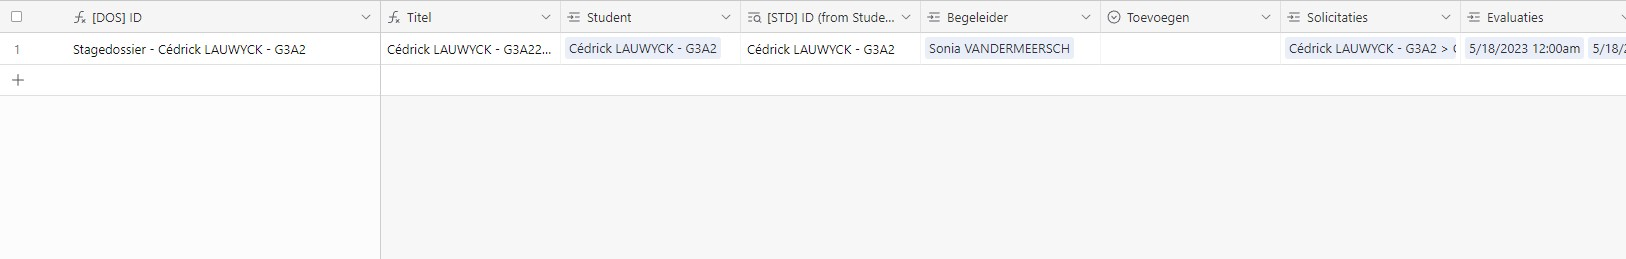
\includegraphics[width=\linewidth]{methodologie/Airtable_tableDossier.jpg}
    \caption{Uitgewerkte 'Dossiers' table in Airtable.}
    \label{fig:meth_airtable_dossiersTable}
\end{figure}


Na het instellen van de attributen, kan overgegaan worden tot de laatste stap in het bouw proces, namelijk automatisaties of workflows invoegen. In tegenstelling tot Podio, zitten deze wel ingebouwd in het platform en zijn ze gemakkelijk te bereiken via één simpele klik. In figuur \ref{fig:meth_airtable_automations} is te zien hoe ze zeer overzichtelijk worden weergegeven. Verder toont de figuur ook hoe een eenvoudige workflow is opgebouwd. In contrast met Podio is er geen apart gedeelte voor filters, maar zitten deze ingebouwd in de configuratie van de trigger,  daarna volgen direct de acties. Bovendien is er ook de optie om een workflow uit te testen, wat in Podio niet het geval is. \\

\begin{figure}[ht]
    \centering
    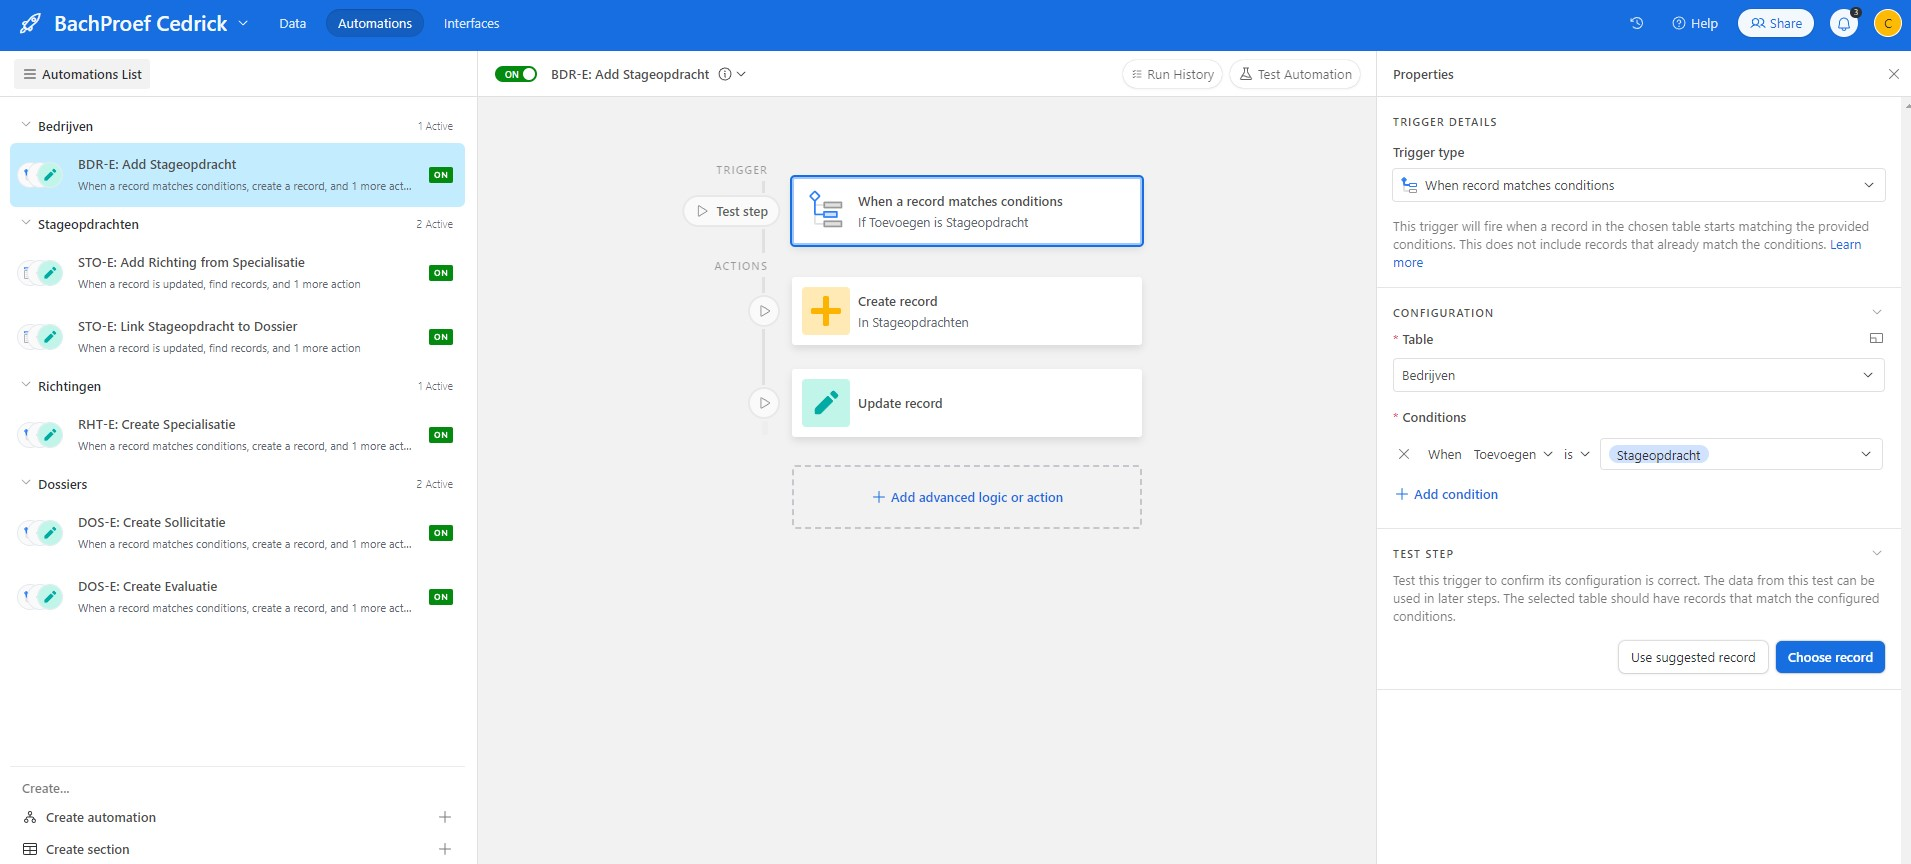
\includegraphics[width=\linewidth]{methodologie/Airtable_automations.jpg}
    \caption{Overzicht van automatisaties in Airtable.}
    \label{fig:meth_airtable_automations}
\end{figure}


Het omzetten tot pdf-bestand daarentegen is in Airtable niet zo eenvoudig dan als in Podio. Airtable voorziet in automatisaties namelijk geen optie om een pdf-bestand op te stellen, maar hier moet dit gebeuren via een extensie. Eerst en vooral is het belangrijk te vermelden dat de optie om extensies toe te voegen, ingebouwd zit in Airtable, wat in Podio niet het geval is. Er zijn verschillende extensies die het opmaken van een pdf-bestand verwezenlijken, zo heb je onder andere de `Page Designer` extensie, die ontwikkeld is door Airtable zelf. Hiermee kan je mooie templates opstellen en invullen met data uit de tabellen. Deze extensie beperkt zich wel tot een enkele pagina, wat dus niet altijd het geval is. Uiteindelijk werd voor deze use case gekozen om gebruik te maken van de `PDF Generator API` extensie. Ook hier wordt vooraf een simpele template opgesteld om vervolgens op te vullen met de gewilde velden uit de dossiers table. Ten slotte hoeven enkel nog de records die geconverteerd moeten worden, geselecteerd worden en kan een pdf-bestand gegenereerd worden. Dat pdf-bestand wordt dan toegevoegd in het `Attachments` veld van de records, zoals weergegeven in figuur \ref{fig:meth_airtable_dossiersAttachments}. Alhoewel hier dus geen automatisatie werd aangemaakt, is het wel degelijk mogelijk om een extensie uit te voeren via een automatisatie. Via de betaalde versie van Airtable kan men in automatisaties scripts toevoegen die het gebruik van extensies toelaat.  \\

\begin{figure}[ht]
    \centering
    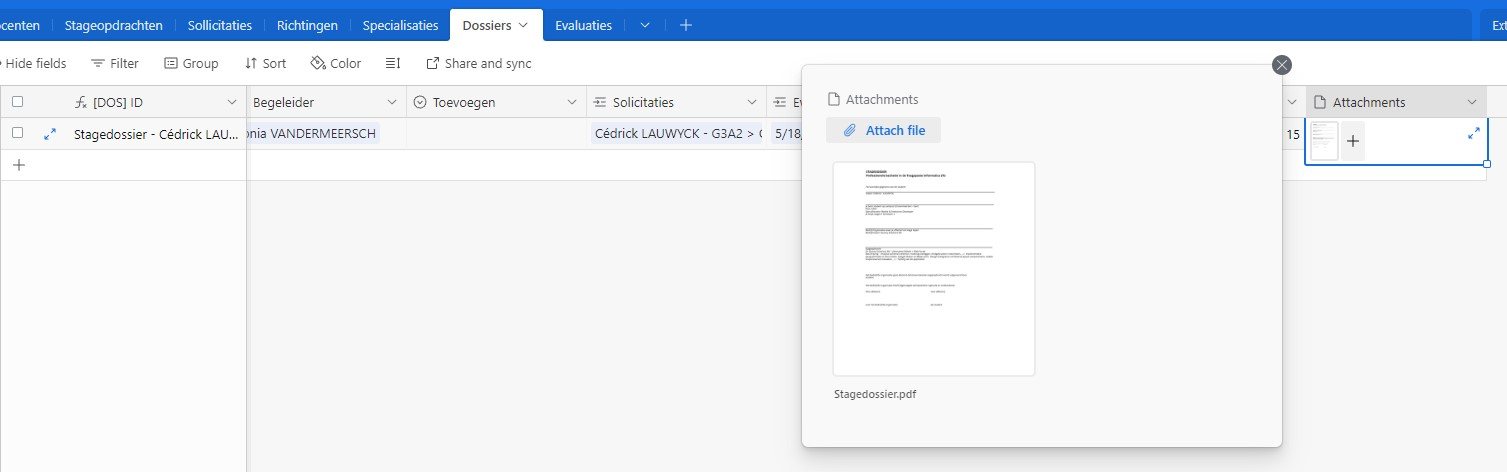
\includegraphics[width=\linewidth]{methodologie/Airtable_dossiersAttachments.jpg}
    \caption{pdf-bestand toegevoegd aan attachments veld in 'Dossiers' table na het uitvoeren van de workflow.}
    \label{fig:meth_airtable_dossiersAttachments}
\end{figure}

Ten slotte kan dus besloten worden dat het perfect mogelijk is om de use case uit te bouwen in Airtable. Ten eerste is het leggen van onderlinge relaties tussen verschillende tabellen zeer goed uitgewerkt, beter dan in Podio om dat er minder over nagedacht moet worden aan welke kant de relatie gelegd wordt. Op gebied van calculaties presteren Airtable en Podio even goed, toch is er voor Podio iets meer technische kennis over JavaScript nodig, terwijl dit in Airtable niet nodig is. Vervolgens is de gebruikerservaring in Airtable heel wat aangenamer dan die van Podio. Desondanks het feit dat in het algemeen een gelijkaardig aantal klikken nodig zijn om een bepaald doel te bereiken, wordt in Airtable nagenoeg geen tijd gebruikt voor het wisselen tussen tabellen, wat te danken is aan hun tabblad-structuur. Bovendien voorziet het platform ook een korte tutorial in het begin, waardoor een gebruiker gemakkelijk op weg geraakt. Verder is de gebruikersinterface of UI zeer mooi opgesteld. De belangrijkste functionaliteiten zijn eenvoudig te bereiken en de gebruiker wordt niet overrompeld door informatie. Een klein nadeel is wel dat er geen overzicht is voor de verschillende activiteiten die gebeuren binnen een workspace. Ten slotte werden tijdens het uitbouwen van de use case geen problemen tegengekomen, alle verliep vlot en de functionaliteiten werkten zoals behoort. \\

\newpage



% APPSHEET __________________________________________________________________________________________________________________________
\subsection{Google AppSheet} % TODO - AppSheet - OK

Nu ook Airtable onderzocht werd, kan overgegaan worden tot het tweede en laatste potentiële alternatief, namelijk Google AppSheet. Eerst en vooral is de structuur in Appsheet opmerkelijk anders dan in Podio of Airtable. Zoals weergegeven in figuur \ref{fig:meth_appsheet_structuur}, maakt het platform namelijk geen gebruik van workspaces en splitst het bovendien projecten op in databases en applicaties. Alhoewel dit iets mindere gebruikerservaring zorgt, omdat er vaak moet afgewisseld worden tussen de twee, heeft dit wel als voordeel dat een enkele database gebruikt kan worden door meerdere applicaties. Bij het aanmaken van een App is er net zoals bij Podio en Airtable de optie om data te importeren van een externe bron, namelijk de Google Drive van de gebruiker. Indien er voor gekozen wordt een blanco app aan te maken, zal Appsheet automatisch ook een achterliggende database creëren. \\

\begin{figure}[ht]
    \centering
    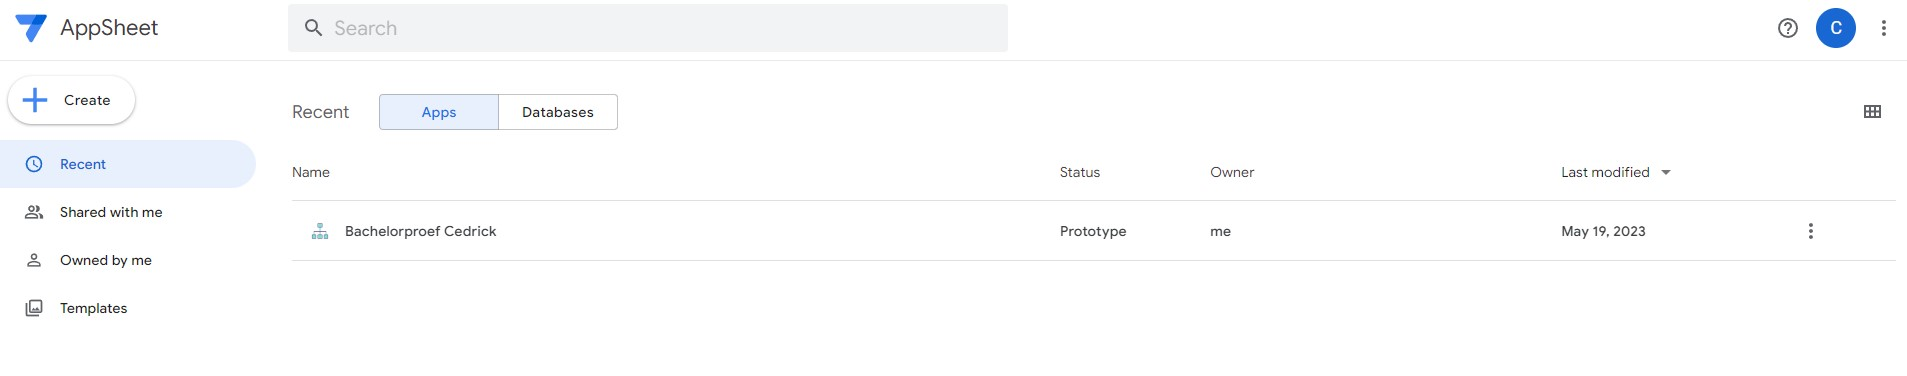
\includegraphics[width=\linewidth]{methodologie/Appsheet_structure.jpg}
    \caption{Structuur van AppSheet.}
    \label{fig:meth_appsheet_structuur}
\end{figure}

% uitleg structuur applicatie
Nadat de applicatie aangemaakt is, moet eerst de database correct geconfigureerd worden. In figuur \ref{fig:meth_appsheet_database} is te zien dat net zoals Airtable ook AppSheet met 'Tables' of tabellen werkt. Voor elk onderwerp uit de analyse wordt dus een tabel aangemaakt. Verder stellen ook de kolommen van de tabel terug de attributen voor, dus wordt voor elk attribuut een kolom aangemaakt. Net zoals bij Airtable en Podio zijn er een groot aantal verschillende velden waaruit gekozen kan worden om het type van een attribuut voor te stellen. In het algemeen bevat AppSheet zelfs meer types velden dan de vorige platformen. Toch ontbreekt er een zeer belangrijk veld, er is namelijk geen calculatie of 'Formula' veld. In Appsheet kunnen berekeningen of tekstverwerkingen niet ingesteld worden in de database zelf, maar gebeurt dit in het applicatie gedeelte, deze worden dus pas achteraf ingesteld. Daarnaast moeten de verschillende kolommen wel nog gelinkt worden met elkaar, dit gebeurt via het `Relationship` veld, dat zeer eenvoudig ingesteld kan worden. Verder heeft ook AppSheet een 'Look-up' veld dat toelaat om data uit een andere tabel weer te geven.

\begin{figure}[ht]
    \centering
    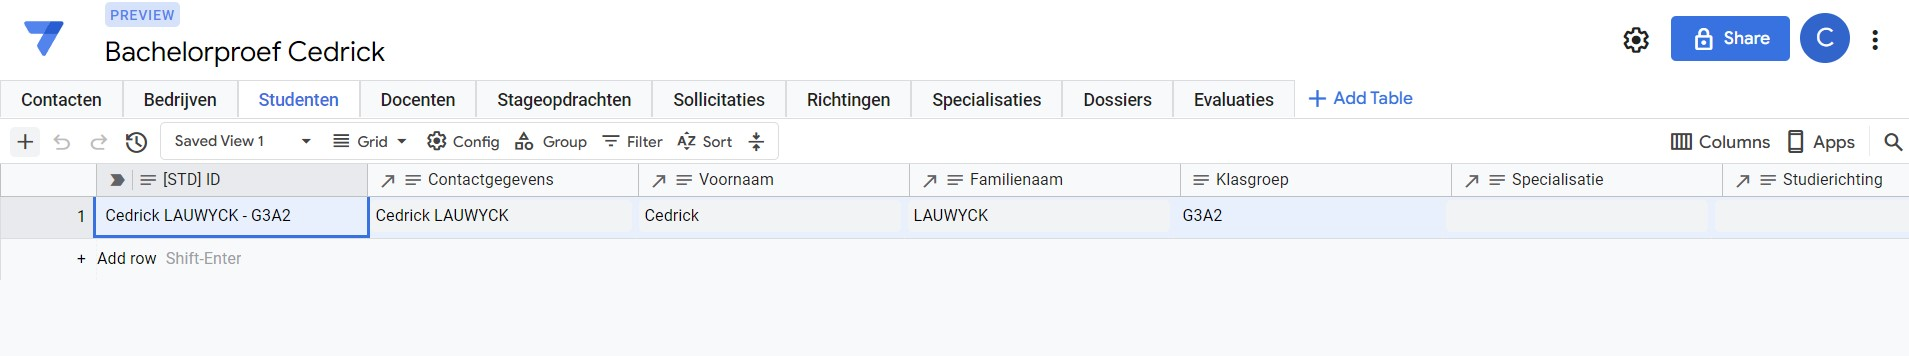
\includegraphics[width=\linewidth]{methodologie/Appsheet_database.jpg}
    \caption{Database in AppSheet.}
    \label{fig:meth_appsheet_database}
\end{figure}

Vervolgens kan overgegaan worden naar het applicatie gedeelte van het bouwproces, waar de formules worden toegevoegd. De structuur van dit deel wordt weergegeven in figuur \ref{fig:meth_appsheet_views} en gaat als volgt. Aan de rechterkant van het scherm wordt altijd een preview van de gebouwde applicatie getoond, de resterende ruimte wordt dan ingevuld met de verschillende configuratie opties. Om data weer te geven in de app, moet eerst een view aangemaakt en toegevoegd worden aan het menu. Een view omvat één tabel uit de database en geeft zijn data weer. Dit kan als verschillende vormen gebeuren, zoals als een gewone lijst of als een dashboard. Bovendien kan data die een 'Address' veld bevat ook weergegeven worden op een map door de ingebouwde Google Maps integratie die AppSheet voorziet. Uiteindelijk wordt dus voor elke tabel die werd aangemaakt in de vorige stappen een view gecreëerd. \\

\begin{figure}[ht]
    \centering
    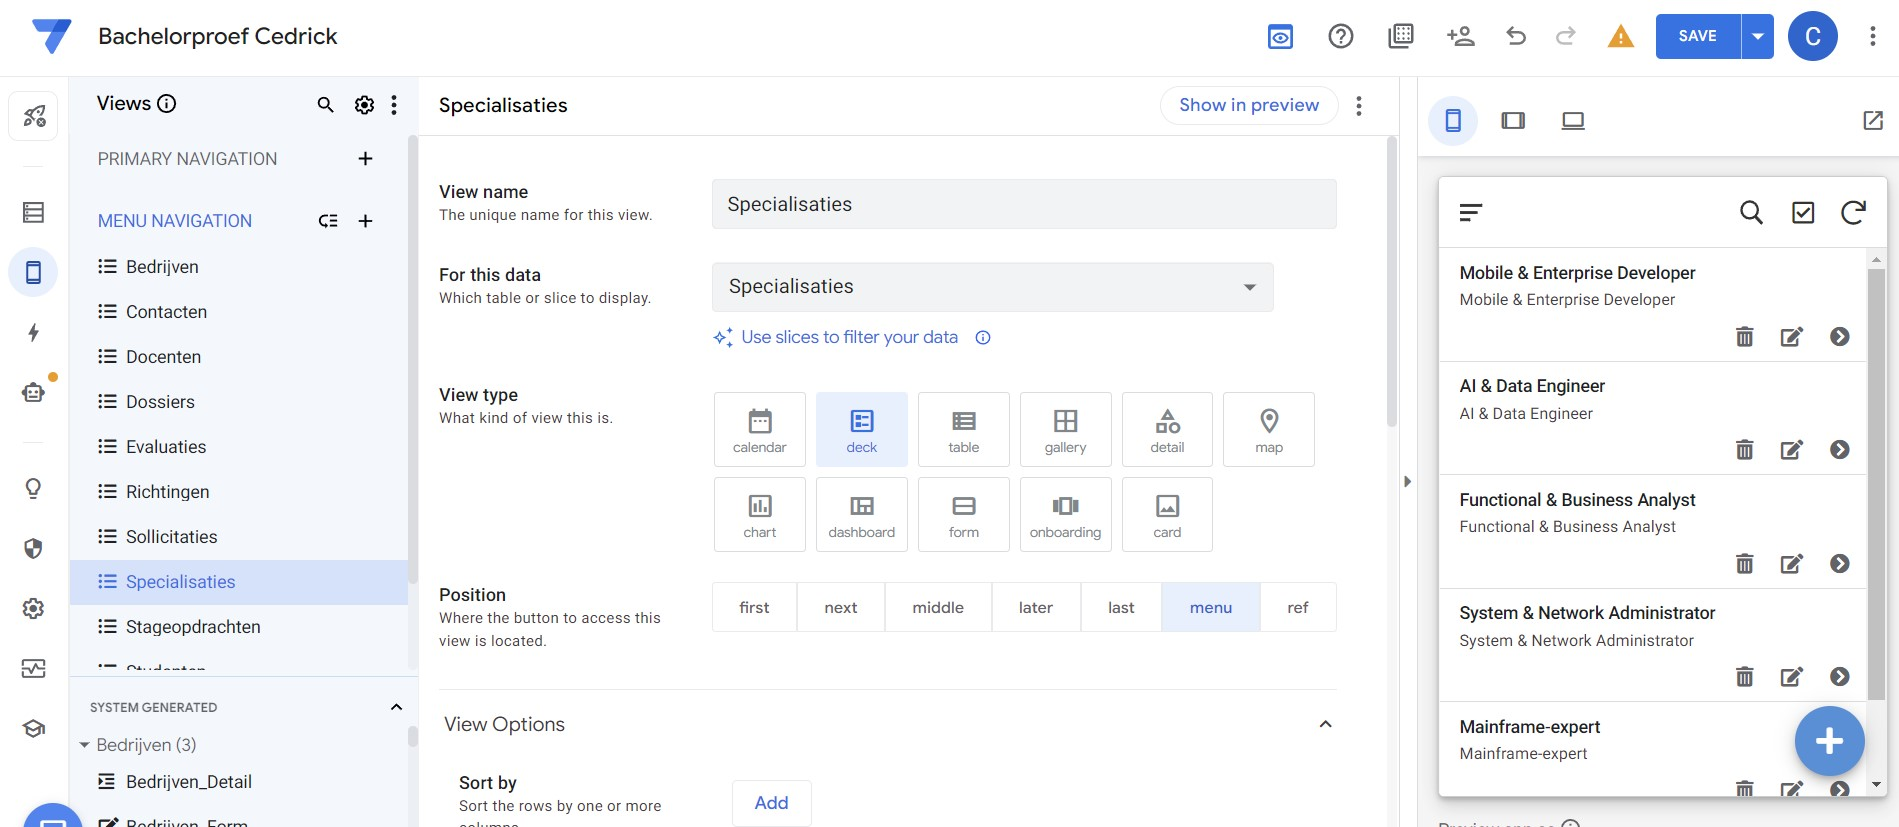
\includegraphics[width=\linewidth]{methodologie/Appsheet_views.jpg}
    \caption{Weergave van data in AppSheet.}
    \label{fig:meth_appsheet_views}
\end{figure}

Nu kunnen formules toegevoegd worden. De eerste stap hierbij is om bij elke tabel op de 'Regenerate schema' knop te klikken. Dit zorgt ervoor dat de verschillende database schema's in de applicatie up-to-date zijn met diegene in de database. Daarna kunnen de nodige formules ingevuld worden, deze zijn vergelijkbaar met formules in Microsoft Excel. In tegenstelling tot Podio kan in Appsheet elk veld als calculatieveld gebruikt worden. In figuur \ref{fig:meth_appsheet_formulas} is te zien hoe bij het invoeren van de calculaties er ook een `Expression Assistant` is die verschillende soorten voorbeeldformules weergeeft en ook de mogelijkheid bied om ze te testen. Daarnaast is er ook een 'Data Explorer' waarmee men gemakkelijk de nodige attributen kan invoeren. Uiteindelijk is het nog belangrijk om te vermelden dat berekeningen in AppSheet geen conditionele logica ondersteunen, wat toch wel een redelijk groot nadeel is. \\

\begin{figure}[ht]
    \centering
    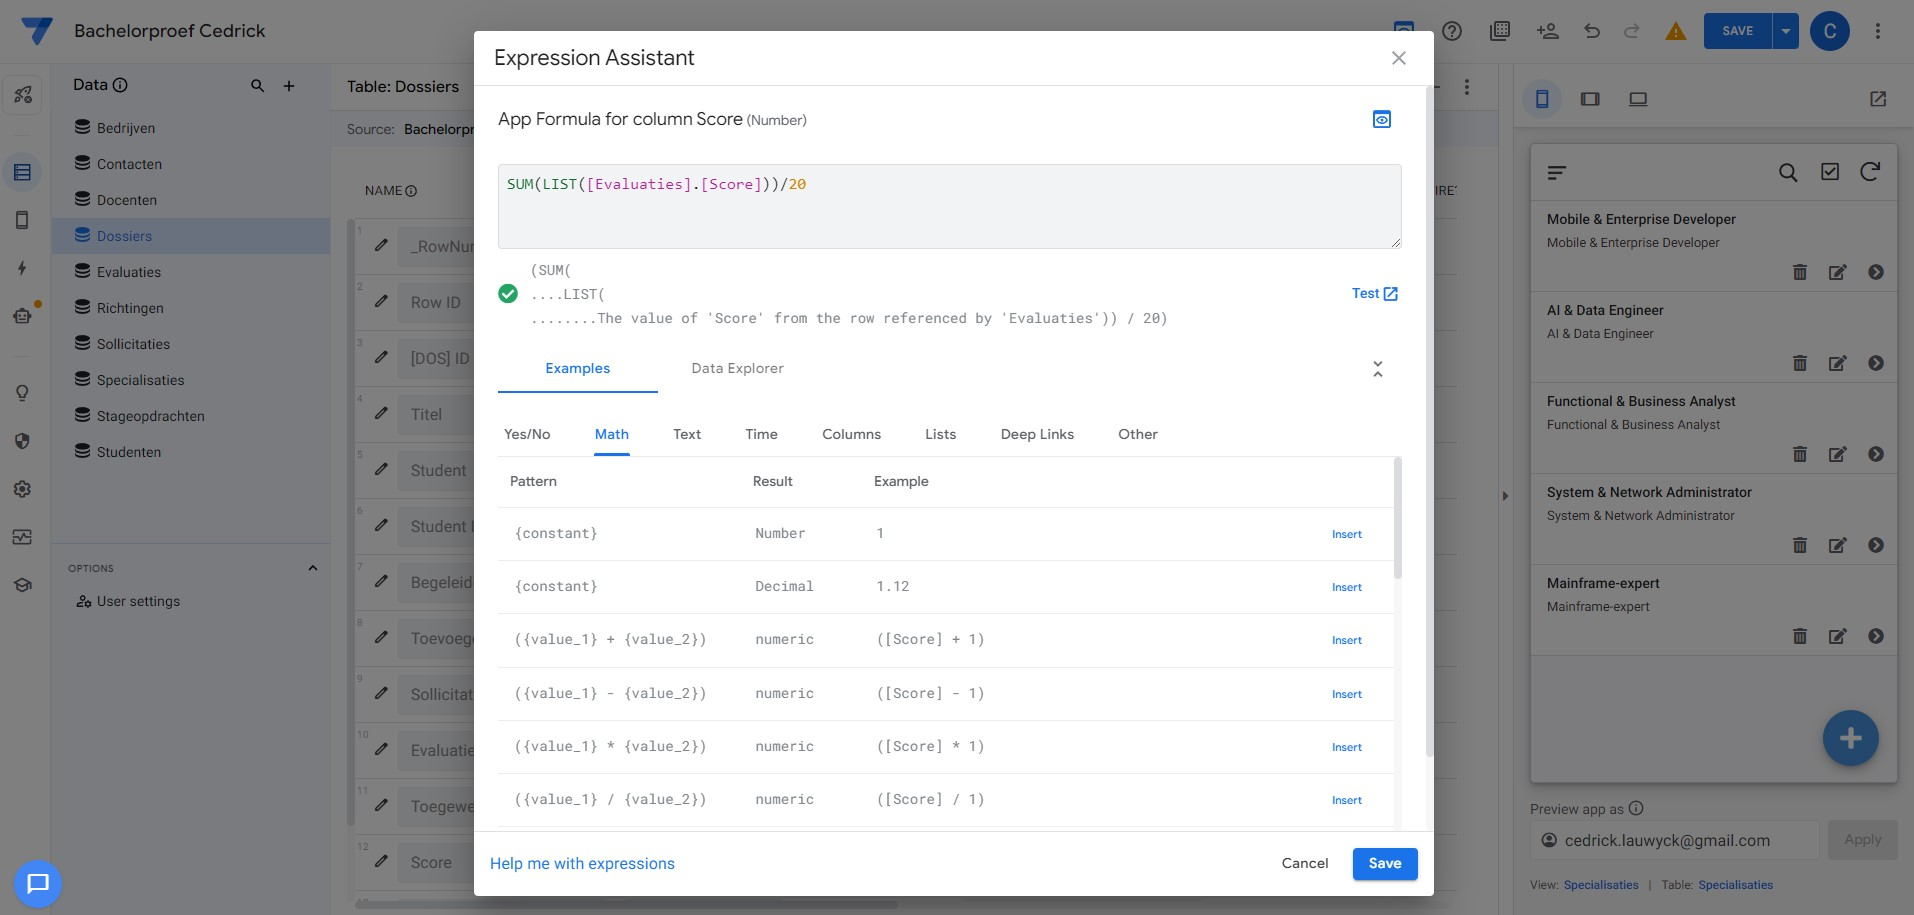
\includegraphics[width=\linewidth]{methodologie/Appsheet_formulaAssistant.jpg}
    \caption{Formules met `Expression Assistant` in Appsheet.}
    \label{fig:meth_appsheet_formulas}
\end{figure}

Een belangrijke opmerking bij Appsheet is dat het aanvullen van de database met gegevens in het applicatiegedeelte gebeurt. Hoewel de mogelijkheid bestaat om rijen toe te voegen in het database gedeelte, zullen op die manier de verschillende formules niet worden toegepast op de data. \\


% automatisaties
Nu kan terug overgegaan worden tot de laatste stap, automatisaties. In Appsheet hoeft enkel de automatisatie voor het omzetten naar pdf-bestand aangemaakt worden. De andere workflows zijn namelijk overbodig, omdat Appsheet al automatisch de mogelijke velden invult indien we op de 'Add'-knop klikken in de applicatie. Automatisaties zijn gemakkelijk te bereiken via een enkele klik op het `robot`-icoontje. Zoals te zien is in figuur \ref{fig:meth_appsheet_automations} wordt een automatisatie in AppSheet gedefinieerd door een zogenaamde `bot`, deze hebben hetzelfde concept als in Podio en Airtable, ze hebben namelijk een set van acties die worden uitgevoerd eens een bepaalde trigger geactiveerd wordt. Voor de use case wordt een bot gezet op de tabel dossiers, met als trigger een verandering in de kolom 'Toevoegen'.
Vervolgens wordt een actie toegevoegd om het dossier om te zetten naar een pdf-bestand. In tegenstelling tot Airtable zit deze functionaliteit net als Podio ingebouwd in AppSheet. Een nadeel is wel dat de gegenereerde pdf achteraf niet zomaar aan het dossier kan worden toegevoegd. Het wordt namelijk opgeslagen op een aparte plaats, zoals Google Drive of OneDrive. Om het bestand te linken aan het dossier, moet een formule worden toegepast op het 'Attachments' veld die verwijst naar de locatie of pad van het pdf-bestand. \\


\begin{figure}[ht]
    \centering
    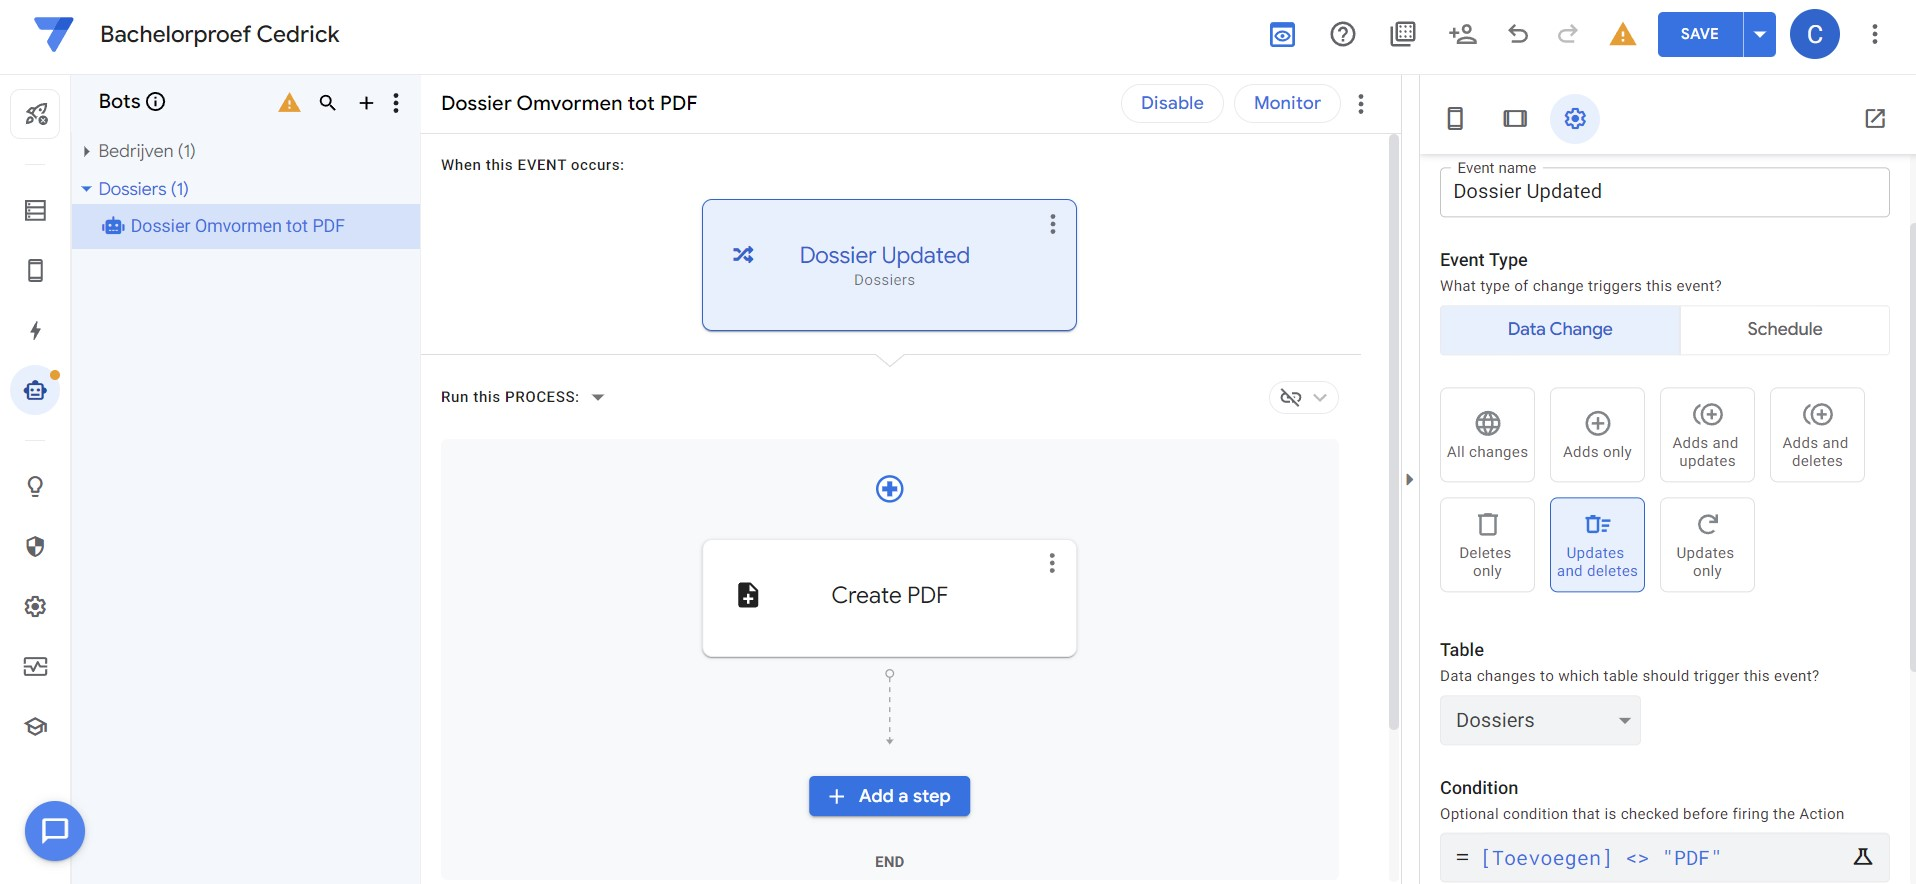
\includegraphics[width=\linewidth]{methodologie/Appsheet_automations.jpg}
    \caption{Automatisaties of 'bots' in Appsheet.}
    \label{fig:meth_appsheet_automations}
\end{figure}


Uiteindelijk is het dus ook perfect mogelijk om de use case uit te bouwen in Appsheet. Net zoals bij Airtable en Podio kunnen er relaties gelegd worden tussen de verschillende tabellen in de database. Verder is het feit dat calculaties op elk veld uitgevoerd kunnen worden een enorm pluspunt, toch is hun functionaliteit beperkter dan de calculatievelden in Podio. Op gebied van gebruikerservaring presteerde Appsheet het minst goed, er waren in het algemeen de meeste klikken\footnote{3 tot 5} en stappen nodig om een doel te bereiken. Daarnaast waren er ook nog extra klikken nodig, zoals het synchroniseren van de database schema's tussen de het applicatie- en databasegedeelte en het heen en weer gaan tussen de 2 delen. Desondanks het feit dat de UI van Appsheet duidelijk opgesteld is, kan ze als onoverzichtelijk overkomen op kleinere schermen, omdat alles dan meer op elkaar gezet wordt en er veel met scrollbars gewerkt moet worden. Ten slotte zijn er ook enkele problemen voorgekomen tijdens het uitwerken van de use case. Vaak waren dit synchronisatie problemen tussen de applicatie en de ingevulde formules. \\



%%=============================================================================
%% Onderzoek
%%=============================================================================

\chapter{\IfLanguageName{dutch}{Onderzoek}{Research}}%
\label{ch:onderzoek}

In voorgaand hoofdstuk werd hoe het onderzoek te werk zal gaan en welke platformen er onderzocht zullen worden, namelijk Airtable en Google AppSheet. In dit hoofdstuk wordt het effectieve onderzoek uitgevoerd, dit betekent dat de use case zal worden uitgebouwd in elk platform. Bovendien worden de verschillende functionaliteiten van de alternatieven besproken en worden op basis van de criteria vergelijkingen gemaakt tussen het alternatief en Podio.

\subsection{Analyse Use Case}

Net zoals bij andere IT projecten is het belangrijk om eerst een analyse uit te voeren voordat er effectief gestart wordt met ontwikkelen. De analyse voor een use case kan verschillen afhangend van het platform waarvoor men ze wil uitvoeren. Aangezien deze studie alternatieven zoekt voor Podio, wordt de analyse fase uitgevoerd in functie van Podio en daarna toegepast op Airtable en Google AppSheet. \\

In Podio wordt een database tabel voorgesteld als een app, die informatie over een bepaald onderwerp bijhoudt. Uit de beschrijving van de use case kan afgeleid worden er op zijn minst 9 apps aanwezig moeten zijn, namelijk studenten, bedrijven, docenten, stageopdrachten, sollicitaties, richtingen, specialisaties, studentendossiers en evaluaties. \\

Het is belangrijk om in te zien dat studenten en docenten beide personen zijn en dat een bedrijf ook meerdere contactpersonen kan hebben. Om een persistente structuur te hebben, is er dus een 10de app genaamd ‘Contacten’ nodig. Bovendien voorkomt dit ook eventuele redundante data. Een docent kan bijvoorbeeld contactpersoon zijn bij een bedrijf, maar dit kan moeilijk aangetoond worden, aangezien er geen expliciete relatie is tussen ‘Bedrijven’ en ‘Docenten’. Deze persoon zou dus twee keer moeten opgeslagen worden in de databank, wat tegenin de richtlijnen van Podio gaat. \\

Daarnaast moet er ook rekening gehouden worden met het leggen van relaties tussen de verschillende apps. In Podio is het bij het 1-op-1 relaties en 1-op-veel relaties beter om de relatie bij slechts één van de twee te apps leggen en bij de andere een calculatie veld te gebruiken. Anders kan er verwarring ontstaan binnenin het platform, indien er bijvoorbeeld een item verwijderd wordt kan de relatie aan één van de kanten nog steeds bestaan. \\

Tenslotte is het belangrijk om na te denken welke automatisaties allemaal toegepast kunnen worden. In dit onderzoek wordt er beperkt tot de volgende;

\begin{itemize}
    \item Automatisch aanmaken van een sollicitatie en linken aan een dossier.
    \item Automatisch aanmaken van een evaluatie en linken een dossier.
    \item Automatisch aanmaken van een stageopdracht en linken aan een bedrijf.
    \item Automatisch invullen van richting wanneer een specialisatie wordt gelinkt aan een stageopdracht.
    \item Automatisch aanmaken van een specialisatie en linken aan een richting.
    \item Dossier automatisch omvormen tot een opgemaakt pdf-bestand.
\end{itemize}

\begin{table}
    \centering
    \caption{\label{tab:Resultaat analyse} }
    \begin{tabular}{ | p{4cm} | p{8cm} | }
        \hline
        \textbf{App} & \textbf{Attributen} \\
        \hline\hline
        Contacten       & (calc.\footnote{calculatie}) ID, voornaam, familienaam, adres, geboortedatum, email, telefoonnummer, (calc.) Bedrijven \\
        Studenten       & (calc.) ID, (rel.\footnote{relatie}) Contact, (rel.) Studierichting, (rel.)  Specialisatie, klasgroep \\
        Bedrijven       & (calc.) ID, naam, adres, email, telefoonnummer, link, (rel.) Contactpersonen, (calc.) Stageopdrachten \\
        Docenten        & (calc.) ID, rol, (rel.) Studierichting \\
        Stageopdrachten & (calc.) ID, titel, (rel.) Bedrijf, beschrijving, (rel.) Richting, (rel.) Specialisaties, periode, aantal-studenten, (rel.) Toegewezen-aan \\
        Sollicitaties   & (calc.) ID, (rel.) Student, (rel.) Bedrijf, datum-gesprek, alleen/medestudent, (rel.) Medestudent, resultaat, opmerking \\
        Richtingen      & (calc.) ID, naam, afkorting, status, (calc.) Specialisaties \\
        Specialisaties  & (calc.) ID, naam-specialisatie, (rel.) Richting \\
        Dossiers        & (calc.) ID, Titel, (rel.) Student, (rel.) Begeleider, (rel.) Sollicitaties, (rel.) Evaluaties, (rel.) Toegewezen-stageopdracht, (calc.) Score \\
        Evaluaties      & (calc.) ID, datum, (rel.) Student. \\
        \hline
    \end{tabular}
\end{table}

Nu de analyse fase voltooid is kan er gestart worden met het ontwikkelen in Podio, Airtable en Google AppSheet. Vervolgens wordt voor elk van de platformen nogmaals de criteria overlopen en wordt er toegelicht hoe goed elk platform eraan voldoet. \\

\newpage



% PODIO __________________________________________________________________________________________________________________________
\subsection{Podio} % TODO - Podio - OK

Vooraleer het bouwproces wordt toegelicht is het belangrijk om nog eens de structuur van Podio op te frissen. In Podio wordt een use case of project weergegeven aan de hand van een workspace. Deze workspace bevat één of meerdere apps die een template voorzien voor een bepaald onderdeel. Een template wordt gebruikt om een item van de app op te bouwen en is een samenstelling van velden zoals een tekstveld, datumveld of calculatieveld. Vanuit een database-perspectief kan een workspace dus gezien worden als de database, een app als een tabel, een template als de kolommen van de tabel en een item als een rij in een tabel. \\

In Podio is de eerste stap van het ontwikkelingsproces dus het aanmaken van de workspace waarin alles gebouwd zal worden. De ‘Activity’ app, zie figuur \ref{fig:meth_podio_workspace}, wordt standaard aangemaakt bij het creëren van een workspace en bevat een overzicht van wat er zich allemaal afspeelt. Indien iets wordt aangepast, wordt dit weergegeven in een tijdslijn samen met de persoon die het heeft aangepast en wanneer de aanpassing verricht werd. Daarnaast wordt ook een kalendertegel en een lijsttegel, met taken die zelf toegevoegd kunnen worden, voorzien. Bovendien is er de optie om zelf tegels toe te voegen die data uit de workspace kunnen weergeven. \\

\begin{figure}[h]
    \centering
    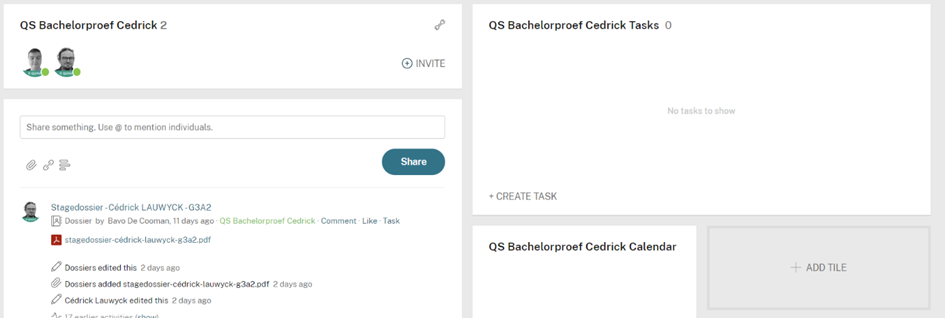
\includegraphics[width=\linewidth]{methodologie/Podio_workspace.png}
    \caption{'Activity' app in een Podio workspace.}
    \label{fig:meth_podio_workspace}
\end{figure}

Nadat de workspace is aangemaakt, kan voor elk onderwerp uit de analyse een app aangemaakt worden. Het is voordeliger om eerste alle apps aan te maken vooraleer de attributen worden toegevoegd, want men kan namelijk geen relatie leggen naar iets dat nog niet bestaat. Dit kan eenvoudig gedaan worden door op de ‘Add App’-knop te klikken, waarna een venster getoond wordt die vraagt achter de naam van de app, de naam van een item en icoon. Voor de benamingen wordt door Quivvy vaak enkelvoud en meervoud gebruikt, ter illustratie: de ‘Contacten’ app heeft ‘Contact’ als naam van het item. Het icoon daarentegen kan gekozen worden uit een uitgebreide lijst van iconen. Het uiteindelijke resultaat van deze stap wordt weergegeven in figuur \ref{fig:meth_podio_lijstApps}. \\

\begin{figure}[ht]
    \centering
    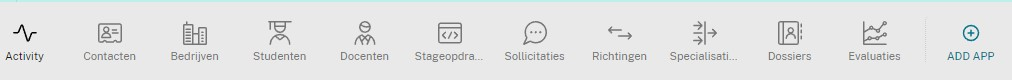
\includegraphics[width=\linewidth]{methodologie/Podio_lijstApps.jpg}
    \caption{Aangemaakte apps in de Podio workspace.}
    \label{fig:meth_podio_lijstApps}
\end{figure}

Eens alle apps aangemaakt zijn, is de fundering van de use case afgewerkt. Nu kan er over gegaan worden tot het instellen van de verschillende attributen en relaties. Dit is mogelijk in 2 simpele klikken, namelijk door naar de app te navigeren en vervolgens via het ‘moersleutel’-icoontje de verschillende instellingen van de openen. Daarna kan men via een derde klik de template van de app gaan bewerken. Zoals eerder vermeld is een template een samenstelling van verschillende types velden die Podio voorziet. Voor de use case wordt dus elk voor elk attribuut van de app een veld toegevoegd. Ter illustratie wordt in figuur \ref{fig:meth_podio_dossierTemplate} de uitgewerkte template voor de 'Dossiers' app van de use case weergegeven. Eerst een vooral werd een calculatieveld toegevoegd voor de ID van het dossier. In dit veld komt het low-code gedeelte van Podio aan bod, het veld accepteert namelijk JavaScript en kan op allerlei manieren gebruikt worden. De laatste lijn in het calculatie veld is wat er uiteindelijk wordt weergegeven, daaronder is ook een preview zichtbaar. In het geval van een dossier wordt een stuk tekst samengevoegd met de ID van de student. Vervolgens wordt een simpel tekstveld gebruikt voor de titel van het dossier, gevolgd door 2 relatievelden om de student en begeleider te linken. Daarna wordt een categorieveld ingevoegd met de opties `Evaluatie` en `Sollicitatie`, dit zal later gebruikt worden voor het toevoegen van een evaluatie of sollicitatie via automatisaties. Podio voorziet namelijk geen knop velden, om die reden wordt een categorie veld gebruikt als workaround. Verder worden nog 2 relatievelden toegevoegd en nog een calculatieveld waarin de totaalscore van de evaluaties wordt uitgerekend en weergegeven. Het is belangrijk om te vermelden dat er voor elk een set van opties beschikbaar zijn, om bijvoorbeeld het veld verplicht te maken of om het aantal relaties in een relatieveld te beperken. \\

\begin{figure}[h]
    \centering
    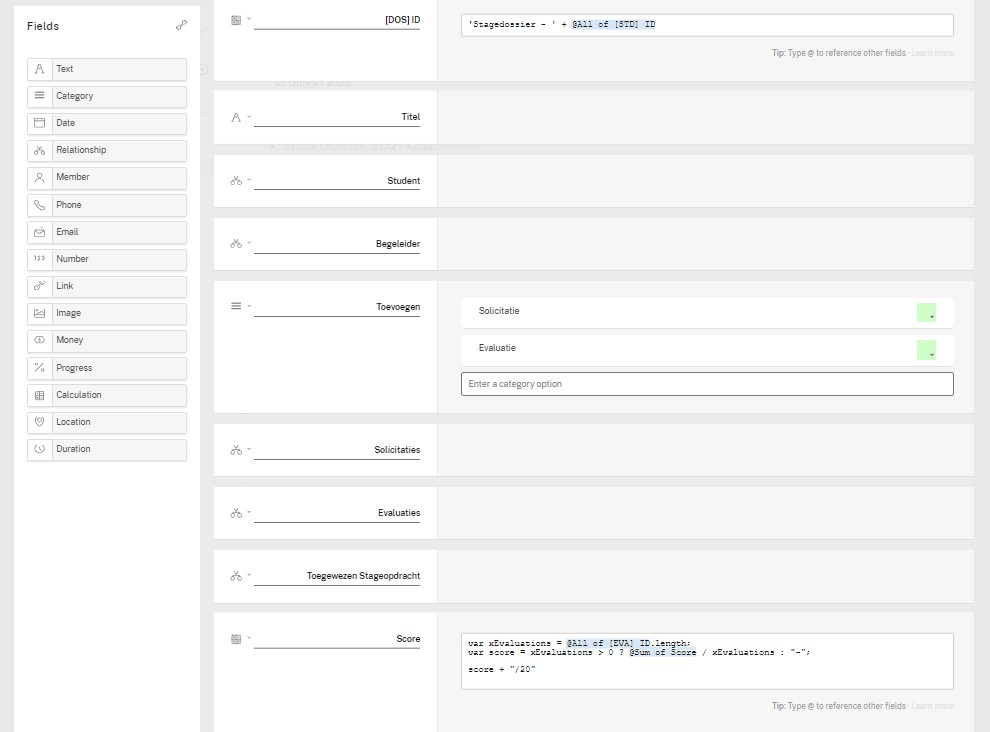
\includegraphics[width=\linewidth]{methodologie/Podio_dossierTemplate.jpg}
    \caption{Uitgewerkte template van de 'Dossier' app.}
    \label{fig:meth_podio_dossierTemplate}
\end{figure}

Om de data mooi weer te geven wordt als extra ook de layout aangepast. Podio voorziet standaard 5 verschillende layouts, namelijk 'Badge', 'Table', 'Card', 'Activity' en 'Calender', verder kunnen ook nog filters ingesteld worden op de attributen van een app. Eens alles geconfigureerd is naar keuze kan ten slotte de weergave als view worden opgeslagen. In figuur \ref{fig:meth_podio_badgeLayout} is een voorbeeld van de badge layout te zien. Bovendien kan men voor elke app via de 'Layout options' selecteren welke velden men wil weergeven op een individuele badge. \\

\begin{figure}[h]
    \centering
    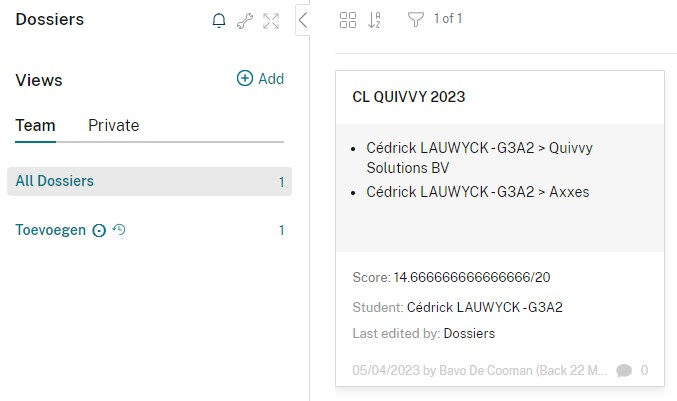
\includegraphics[width=\linewidth]{methodologie/Podio_badgeLayout.jpg}
    \caption{Badge layout in Podio.}
    \label{fig:meth_podio_badgeLayout}
\end{figure}

De volgende stap is om de automatisaties of workflows toe te voegen, dit gebeurt via Globiflow\footnote{wordt ook wel Citrix Podio Workflow Automation genoemd.}, een geavanceerde workflow automation tool gemaakt voor Podio. Door naar de instellingen van een willekeurige app te navigeren en vervolgens door te klikken op `workflow automations`, wordt men omgeleid naar een externe pagina waar automatisaties kunnen worden ingesteld. Eerst en vooral is het belangrijk om onderaan de pagina op de 'Refresh from Podio' knop te klikken, deze zorgt er namelijk voor dat de laatst opgeslagen configuratie van de Podio workspace wordt opgehaald. Nu alle apps en bijkomende velden aanwezig zijn, kunnen er workflows aangemaakt worden. Deze bevatten een trigger, een set van filters en een set van acties die worden uitgevoerd. Er zal dus voor elke automatisatie in de analyse, een workflow aangemaakt worden. Een handige feature van Globiflow, is dat het voor elke workflow ook een verkorte versie of recept weergeeft. Bovendien wordt ook een schatting weergegeven van hoeveel minuten er bespaard worden door de workflow uit te voeren. \\

In figuur \ref{fig:meth_podio_workflow} is terug een uitgewerkt voorbeeld te zien, namelijk het omvormen van een dossier tot pdf bestand. De trigger voor deze workflow is het updaten van een dossier, in de filters wordt dit dan verfijnd tot het updaten van het 'verwerken' veld. Eens dit op `Omzetten naar PDF` wordt gezet, zal de flow verdergaan naar de acties, bij een andere waarde wordt de flow beëindigt. Bij de eerste actie wordt een variabele opgeslagen met het jaartal van creatiedatum van het dossier, deze zal dan later gebruikt worden in de template voor het omvormen naar PDF. Vervolgens wordt de data van enkele referenties opgehaald, namelijk de informatie over de student, studierichting en het bedrijf. Daarna komt het omzetten naar PDF bestand, men kan volledig zelf een template opbouwen met alle nodige informatie uit Podio. Bovendien is het ook mogelijk om een footer en header in te stellen, voor onze use case wordt in de footer bijvoorbeeld informatie over Hogeschool Gent weergegeven. Er hoeft geen actie toegevoegd te worden om de gemaakte PDF aan het item zelf te hangen, want dit zit namelijk inbegrepen in de actie. Indien men het bestand zou willen doormailen kan dat eenvoudig door vanuit deze workflow een andere workflow te activeren en vervolgens de PDF mee te geven. De voorlaatste stap van automatisatie is het `Dossier` item terug updaten om het 'Toevoegen' veld terug op leeg te zetten. Ten slotte worden nog enkele acties toegevoegd om de referenties die eerder werden opgehaald terug op te ruimen, eens dit gebeurt is, is de workflow afgewerkt. \\

\begin{figure}[h]
    \centering
    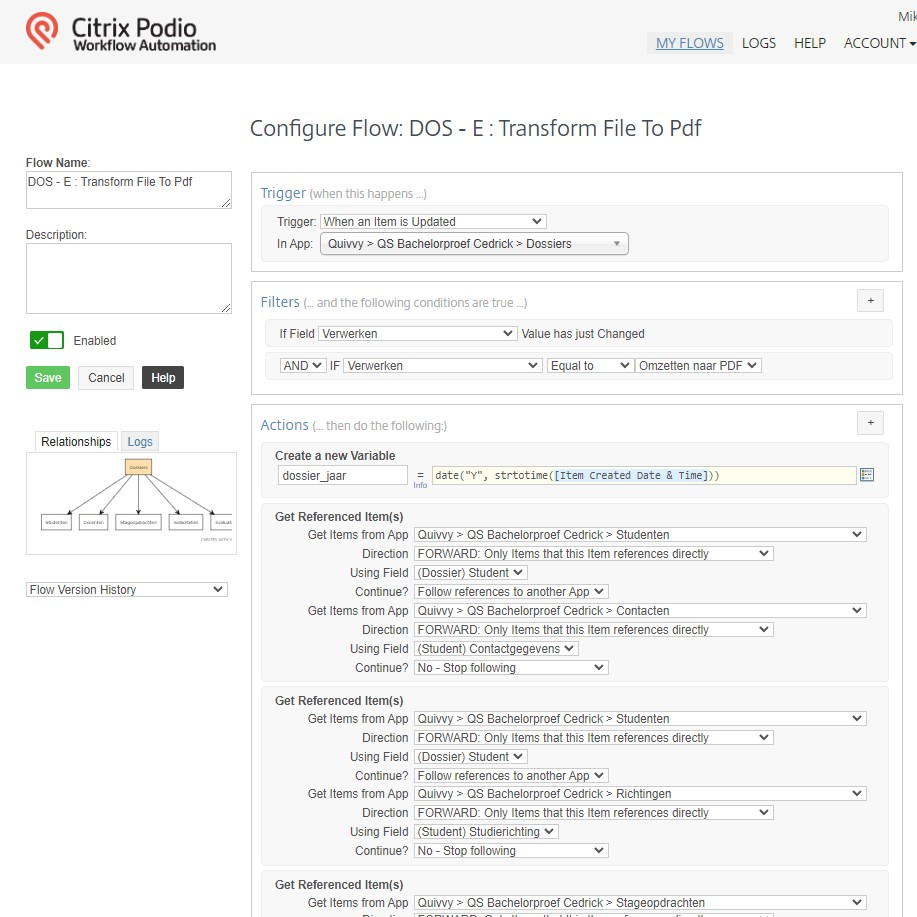
\includegraphics[width=\linewidth]{methodologie/Podio_workflow.jpg}
    \caption{Workflow in Globiflow.}
    \label{fig:meth_podio_workflow}
\end{figure}

Nu de use case is voltooid in Podio, is het belangrijk om de criteria eens door te nemen en kort te evalueren hoe goed het platform presteert. Allereerst is het heel eenvoudig om relaties te leggen via het relatieveld, hoewel er wel altijd nagedacht moet worden aan welke kant de relatie wordt gelegd. Ten tweede kunnen workflows ook gemakkelijk worden ingesteld. Alles heeft een duidelijke benaming, waardoor zelfs lange reeksen van acties eenvoudig te begrijpen zijn. Bovendien biedt Podio een zeer prettige gebruikerservaring. De verschillende knoppen en functies zijn gemakkelijk te begrijpen en kunnen met slechts 1 tot 4 klikken worden bereikt. \\

Het uitbouwen van de use case is echter niet zonder problemen verlopen. Bijvoorbeeld, het instellen van de 'layout options' voor een badge moest vaak twee keer worden toegepast, omdat ze de eerste keer niet werden opgeslagen in het systeem. \\

\newpage



% AIRTABLE __________________________________________________________________________________________________________________________
\subsection{Airtable} % TODO - Airtable - OK

Nu de use case uitgewerkt is in Podio kan overgegaan worden naar het eerste potentiële alternatief, Airtable. De structuur van Airtable is gelijkaardig aan die van Podio, ook hier wordt weer gewerkt met workspaces. In een workspace kan dan een base of database worden aangemaakt, deze zal alle data van de use case omvatten. Verder bestaat een base uit zogenaamde `Tables` of tabellen, die vergelijkbaar zijn met apps uit Podio of dus met een tabel in een database. Voor elk onderwerp uit de analyse wordt dus een tabel toegevoegd, de attributen of kolommen zullen later ingesteld worden. Bij het aanmaken wordt er gekozen om een lege tabel aan te creëren. Daarnaast voorziet Airtable net zoals Podio ook de optie om een tabel aan te maken gebaseerd op een csv-bestand\footnote{simpel bestandsformaat om tabulaire data op te slaan}. Daarnaast kan er ook data uit verschillende andere bronnen zoals Google Drive, Salesforce of Jira Server,$\ldots$ Wat niet standaard ingebouwd zit in Podio. \\

Wanneer alle tabellen aangemaakt zijn, ziet de structuur eruit zoals in figuur \ref{fig:meth_airtable_tables}. Airtable maakt gebruik van een tabblad structuur, waardoor er geen nieuwe pagina moet worden ingeladen om te wisselen van tabel, dit zorgt dan weer voor een zeer aangename gebruikerservaring. \\

\begin{figure}[h]
    \centering
    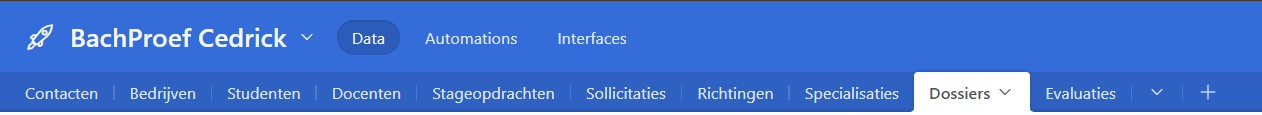
\includegraphics[width=\linewidth]{methodologie/Airtable_tables.jpg}
    \caption{Tables in Airtable.}
    \label{fig:meth_airtable_tables}
\end{figure}

Eens de vorige stap voltooid is, kunnen de attributen per tabel worden ingesteld. In Airtable stelt elke kolom van een tabel een attribuut voor. Om die redenen zijn er dus ook verschillende soorten velden, zoals een `Email` veld om e-mail bij te houden of een 'Phone' veld om een telefoonnummer bij te houden. Een klein verschil met Podio is dat Airtable geen speciaal veld om een adres op te slaan voorziet. Dit is toch wel belangrijk en maakt het bijhouden van een adres minder eenvoudig, aangezien dit dus door een gewoon tekstveld moet gebeuren. \\

De twee belangrijkste types velden zijn het `Relationship` veld en het `Formula` veld. Zoals de naam impliceert, wordt het `Relationship` veld gebruikt om, net zoals in Podio, relaties te leggen tussen de verschillende tabellen. Relaties op zich zijn goed uitgewerkt in Airtable, in tegenstelling tot Podio worden ze direct aan beide kanten toegevoegd. Dit betekent dat als er bijvoorbeeld in de `Specialisaties` tabel een link gelegd wordt naar `Richtingen`, dan zal er ook automatisch een veld worden toegevoegd in de tabel van 'Richtingen'. Bovendien kan er net zoals in Podio gekozen worden of het veld één of meerdere referenties mag bevatten. Verder heeft Airtable ook nog het `Lookup` veld, waarmee een waarde uit een andere tabel kan worden weergegeven. Om dit in Podio te bereiken zou een calculatie veld gebruikt moeten worden. \\

Het 'Formula' veld is vergelijkbaar met een calculatieveld in Podio. Hiermee kunnen aangepaste formules gemaakt worden op basis van andere velden in dezelfde table. Bovendien ondersteunt het veld een groot aantal functies en operatoren, waaronder wiskundige, logische en tekstfuncties. Verder is ook conditionele logica zoals een 'if-else' structuur mogelijk binnen dit veld. Kortom is het dus een krachtig hulpmiddel voor gegevensverwerking binnen Airtable.  In de use case wordt dit type veld vooral gebruikt om de ID's van de verschillende tabellen te berekenen. \\

In figuur \ref{fig:meth_airtable_dossiersTable} is de uitgewerkte tabel voor de 'Dossiers' weergegeven, waarvan structuur van de opzet is nagenoeg dezelfde als die in Podio, op enkele verschillen na. Zo wordt voor de totaal score bijvoorbeeld gebruik gemaakt van een ander soort veld dan het `Formula` veld. In tegenstelling tot Podio ondersteunt het `Formula` veld geen loops, in plaats daarvan voorziet Airtable het `Roll-up` veld. Met dit veld kan een lijst met waarden, afkomstige uit een relatie, worden verwerkt. Zo wordt voor de totaalscore de som gemaakt van elke score bij de evaluaties en daarna gedeeld door 20. \\ 

\begin{figure}[h]
    \centering
    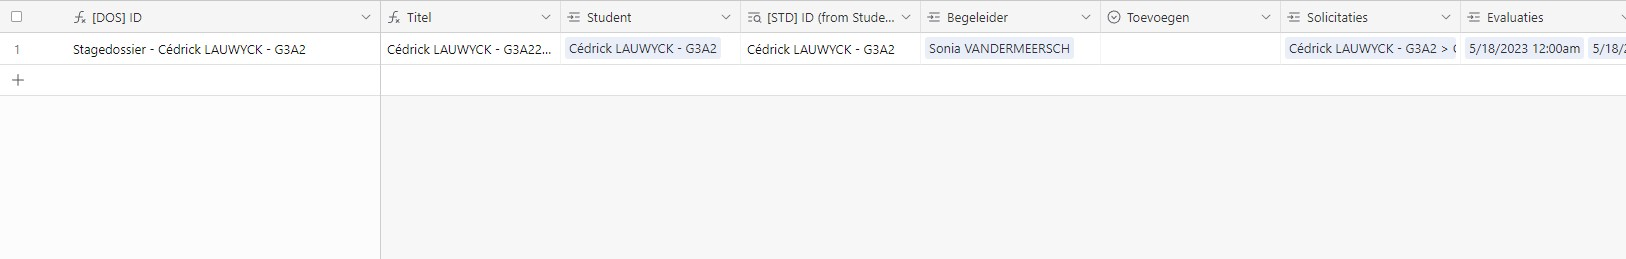
\includegraphics[width=\linewidth]{methodologie/Airtable_tableDossier.jpg}
    \caption{Uitgewerkte 'Dossiers' table in Airtable.}
    \label{fig:meth_airtable_dossiersTable}
\end{figure}


Na het instellen van de attributen, kan overgegaan worden tot de laatste stap in het bouw proces, namelijk automatisaties of workflows invoegen. In tegenstelling tot Podio, zitten deze wel ingebouwd in het platform en zijn ze gemakkelijk te bereiken via één simpele klik. In figuur \ref{fig:meth_airtable_automations} is te zien hoe ze zeer overzichtelijk worden weergegeven. Verder toont de figuur ook hoe een eenvoudige workflow is opgebouwd. In contrast met Podio is er geen apart gedeelte voor filters, maar zitten deze ingebouwd in de configuratie van de trigger,  daarna volgen direct de acties. Bovendien is er ook de optie om een workflow uit te testen, wat in Podio niet het geval is. \\

\begin{figure}[h]
    \centering
    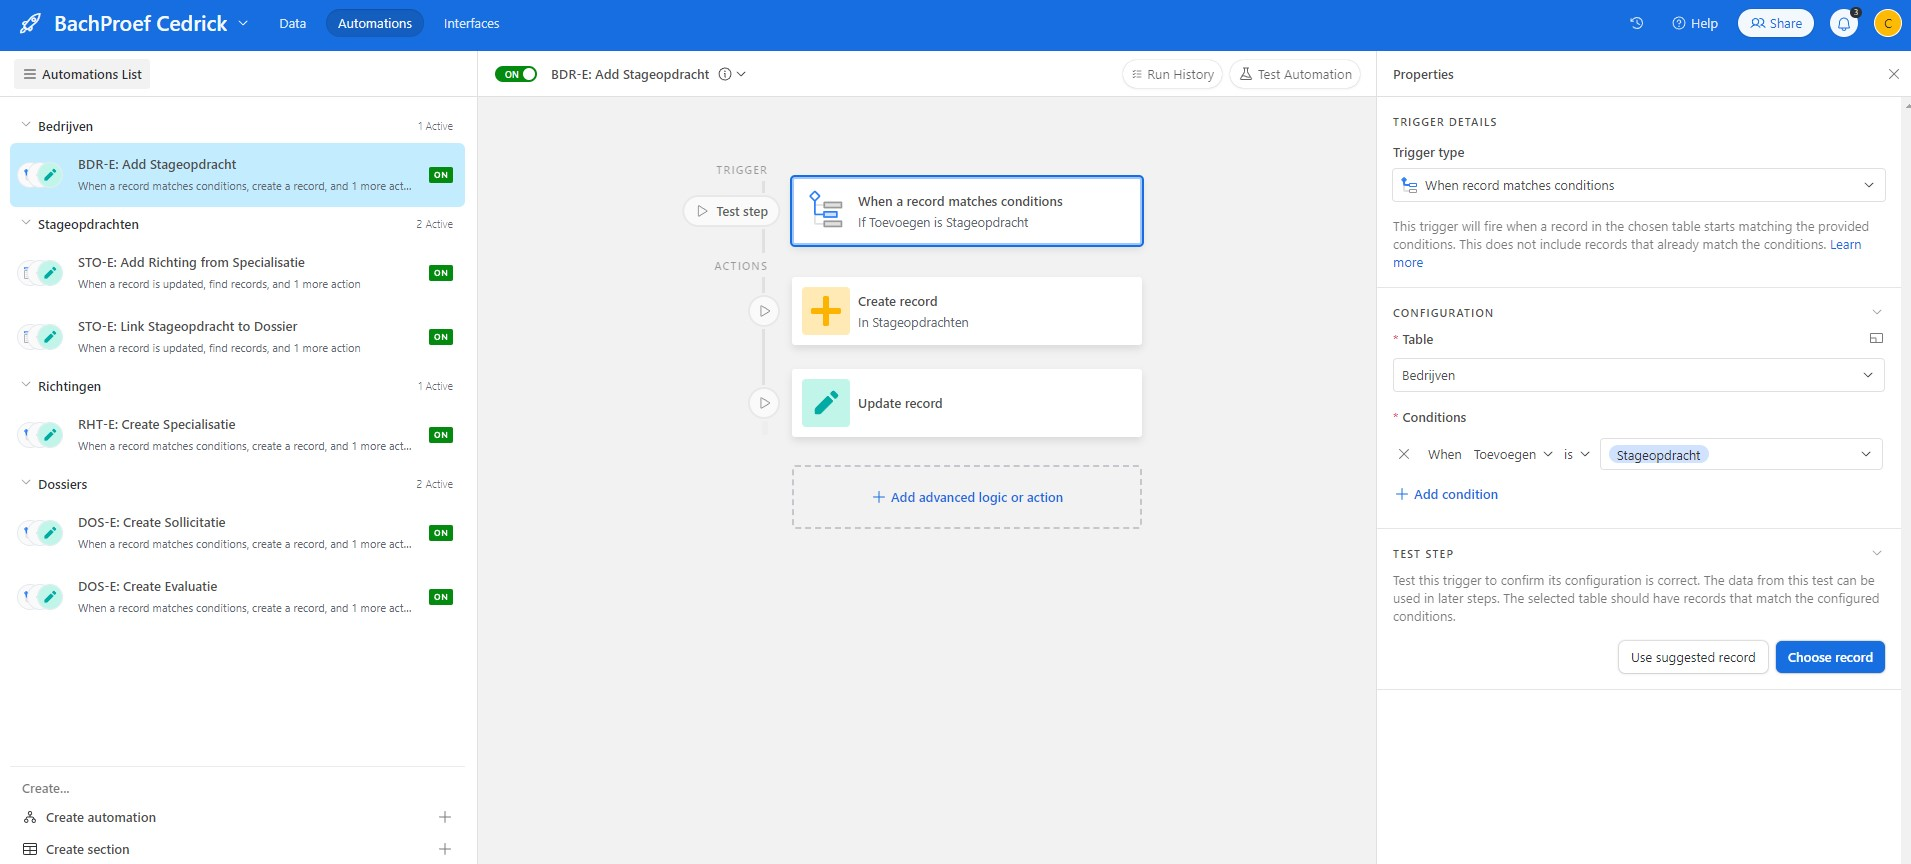
\includegraphics[width=\linewidth]{methodologie/Airtable_automations.jpg}
    \caption{Overzicht van automatisaties in Airtable.}
    \label{fig:meth_airtable_automations}
\end{figure}


Het omzetten tot pdf-bestand daarentegen is in Airtable niet zo eenvoudig dan als in Podio. Airtable voorziet in automatisaties namelijk geen optie om een pdf-bestand op te stellen, maar hier moet dit gebeuren via een extensie. Eerst en vooral is het belangrijk te vermelden dat de optie om extensies toe te voegen, ingebouwd zit in Airtable, wat in Podio niet het geval is. Er zijn verschillende extensies die het opmaken van een pdf-bestand verwezenlijken, zo heb je onder andere de `Page Designer` extensie, die ontwikkeld is door Airtable zelf. Hiermee kan je mooie templates opstellen en invullen met data uit de tabellen. Deze extensie beperkt zich wel tot een enkele pagina, wat dus niet altijd het geval is. Uiteindelijk werd voor deze use case gekozen om gebruik te maken van de `PDF Generator API` extensie. Ook hier wordt vooraf een simpele template opgesteld om vervolgens op te vullen met de gewilde velden uit de dossiers table. Ten slotte hoeven enkel nog de records die geconverteerd moeten worden, geselecteerd worden en kan een pdf-bestand gegenereerd worden. Dat pdf-bestand wordt dan toegevoegd in het `Attachments` veld van de records, zoals weergegeven in figuur \ref{fig:meth_airtable_dossiersAttachments}. Alhoewel hier dus geen automatisatie werd aangemaakt, is het wel degelijk mogelijk om een extensie uit te voeren via een automatisatie. Via de betaalde versie van Airtable kan men in automatisaties scripts toevoegen die het gebruik van extensies toelaat.  \\

\begin{figure}[h]
    \centering
    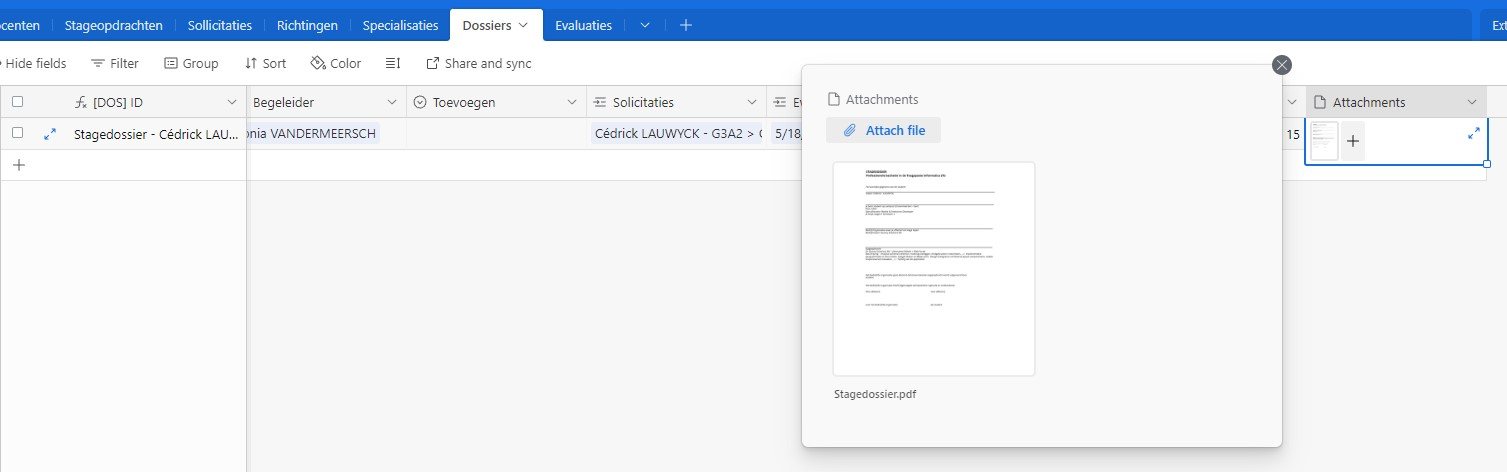
\includegraphics[width=\linewidth]{methodologie/Airtable_dossiersAttachments.jpg}
    \caption{pdf-bestand toegevoegd aan attachments veld in 'Dossiers' table na het uitvoeren van de workflow.}
    \label{fig:meth_airtable_dossiersAttachments}
\end{figure}

Ten slotte kan dus besloten worden dat het perfect mogelijk is om de use case uit te bouwen in Airtable. Ten eerste is het leggen van onderlinge relaties tussen verschillende tabellen zeer goed uitgewerkt, beter dan in Podio om dat er minder over nagedacht moet worden aan welke kant de relatie gelegd wordt. Op gebied van calculaties presteren Airtable en Podio even goed, toch is er voor Podio iets meer technische kennis over JavaScript nodig, terwijl dit in Airtable niet nodig is. Vervolgens is de gebruikerservaring in Airtable heel wat aangenamer dan die van Podio. Desondanks het feit dat in het algemeen een gelijkaardig aantal klikken nodig zijn om een bepaald doel te bereiken, wordt in Airtable nagenoeg geen tijd gebruikt voor het wisselen tussen tabellen, wat te danken is aan hun tabblad-structuur. Bovendien voorziet het platform ook een korte tutorial in het begin, waardoor een gebruiker gemakkelijk op weg geraakt. Verder is de gebruikersinterface of UI zeer mooi opgesteld. De belangrijkste functionaliteiten zijn eenvoudig te bereiken en de gebruiker wordt niet overrompeld door informatie. Een klein nadeel is wel dat er geen overzicht is voor de verschillende activiteiten die gebeuren binnen een workspace. Ten slotte werden tijdens het uitbouwen van de use case geen problemen tegengekomen, alle verliep vlot en de functionaliteiten werkten zoals behoort. \\

\newpage



% APPSHEET __________________________________________________________________________________________________________________________
\subsection{Google AppSheet} % TODO - AppSheet - OK

Nu ook Airtable onderzocht werd, kan overgegaan worden tot het tweede en laatste potentiële alternatief, namelijk Google AppSheet. Eerst en vooral is de structuur in Appsheet opmerkelijk anders dan in Podio of Airtable. Zoals weergegeven in figuur \ref{fig:meth_appsheet_structuur}, maakt het platform namelijk geen gebruik van workspaces en splitst het bovendien projecten op in databases en applicaties. Alhoewel dit iets mindere gebruikerservaring zorgt, omdat er vaak moet afgewisseld worden tussen de twee, heeft dit wel als voordeel dat een enkele database gebruikt kan worden door meerdere applicaties. Bij het aanmaken van een App is er net zoals bij Podio en Airtable de optie om data te importeren van een externe bron, namelijk de Google Drive van de gebruiker. Indien er voor gekozen wordt een blanco app aan te maken, zal Appsheet automatisch ook een achterliggende database creëren. \\

\begin{figure}[h]
    \centering
    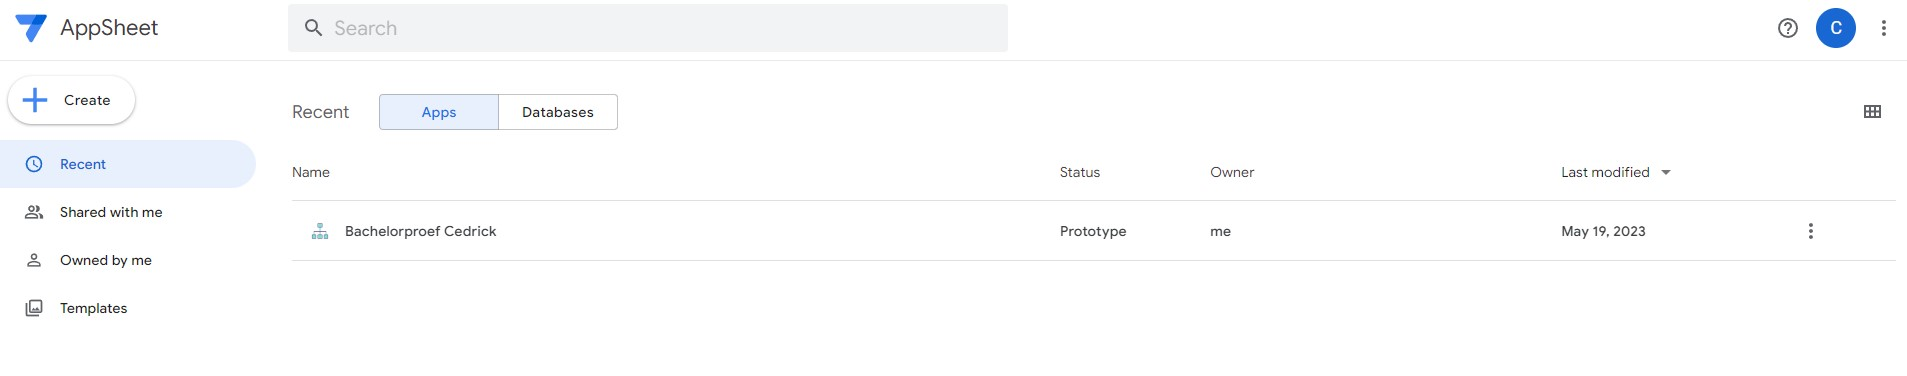
\includegraphics[width=\linewidth]{methodologie/Appsheet_structure.jpg}
    \caption{Structuur van AppSheet.}
    \label{fig:meth_appsheet_structuur}
\end{figure}

% uitleg structuur applicatie
Nadat de applicatie aangemaakt is, moet eerst de database correct geconfigureerd worden. In figuur \ref{fig:meth_appsheet_database} is te zien dat net zoals Airtable ook AppSheet met 'Tables' of tabellen werkt. Voor elk onderwerp uit de analyse wordt dus een tabel aangemaakt. Verder stellen ook de kolommen van de tabel terug de attributen voor, dus wordt voor elk attribuut een kolom aangemaakt. Net zoals bij Airtable en Podio zijn er een groot aantal verschillende velden waaruit gekozen kan worden om het type van een attribuut voor te stellen. In het algemeen bevat AppSheet zelfs meer types velden dan de vorige platformen. Toch ontbreekt er een zeer belangrijk veld, er is namelijk geen calculatie of 'Formula' veld. In Appsheet kunnen berekeningen of tekstverwerkingen niet ingesteld worden in de database zelf, maar gebeurt dit in het applicatie gedeelte, deze worden dus pas achteraf ingesteld. Daarnaast moeten de verschillende kolommen wel nog gelinkt worden met elkaar, dit gebeurt via het `Relationship` veld, dat zeer eenvoudig ingesteld kan worden. Verder heeft ook AppSheet een 'Look-up' veld dat toelaat om data uit een andere tabel weer te geven.

\begin{figure}[h]
    \centering
    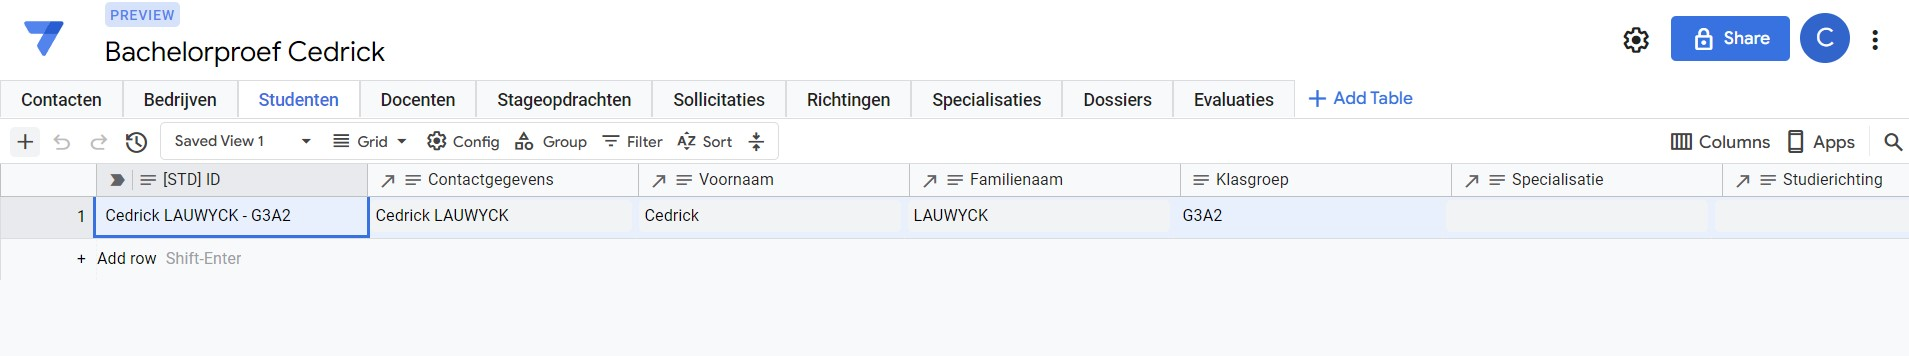
\includegraphics[width=\linewidth]{methodologie/Appsheet_database.jpg}
    \caption{Database in AppSheet.}
    \label{fig:meth_appsheet_database}
\end{figure}

Vervolgens kan overgegaan worden naar het applicatie gedeelte van het bouwproces, waar de formules worden toegevoegd. De structuur van dit deel wordt weergegeven in figuur \ref{fig:meth_appsheet_views} en gaat als volgt. Aan de rechterkant van het scherm wordt altijd een preview van de gebouwde applicatie getoond, de resterende ruimte wordt dan ingevuld met de verschillende configuratie opties. Om data weer te geven in de app, moet eerst een view aangemaakt en toegevoegd worden aan het menu. Een view omvat één tabel uit de database en geeft zijn data weer. Dit kan als verschillende vormen gebeuren, zoals als een gewone lijst of als een dashboard. Bovendien kan data die een 'Address' veld bevat ook weergegeven worden op een map door de ingebouwde Google Maps integratie die AppSheet voorziet. Uiteindelijk wordt dus voor elke tabel die werd aangemaakt in de vorige stappen een view gecreëerd. \\

\begin{figure}[ht]
    \centering
    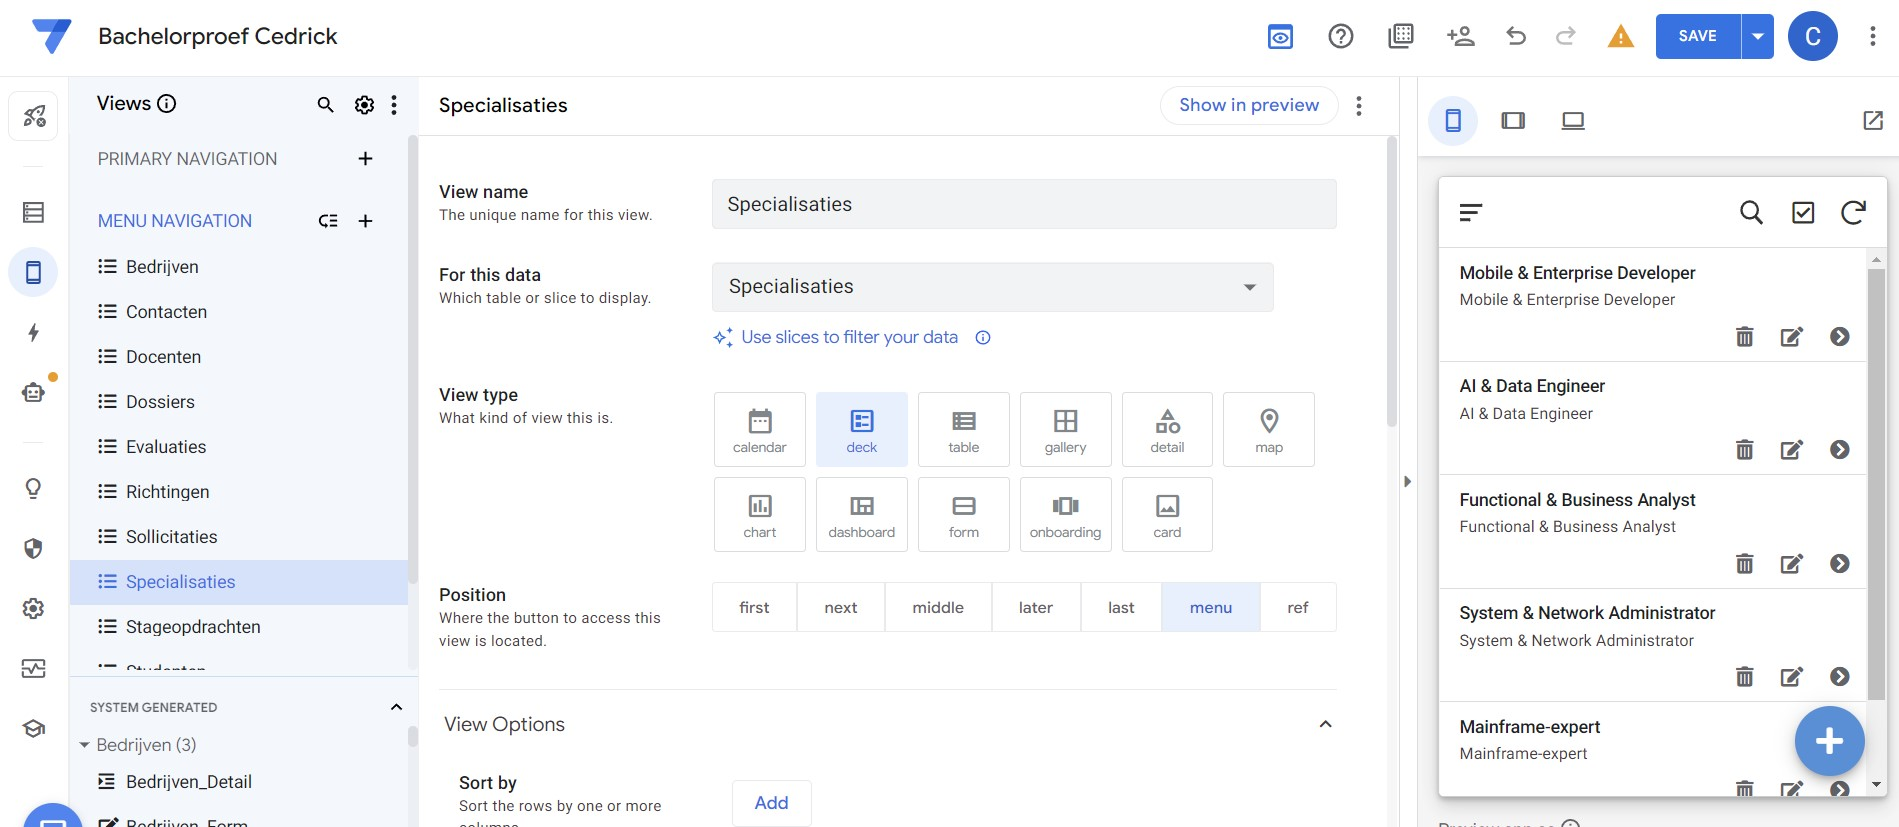
\includegraphics[width=\linewidth]{methodologie/Appsheet_views.jpg}
    \caption{Weergave van data in AppSheet.}
    \label{fig:meth_appsheet_views}
\end{figure}

Nu kunnen formules toegevoegd worden. De eerste stap hierbij is om bij elke tabel op de 'Regenerate schema' knop te klikken. Dit zorgt ervoor dat de verschillende database schema's in de applicatie up-to-date zijn met diegene in de database. Daarna kunnen de nodige formules ingevuld worden, deze zijn vergelijkbaar met formules in Microsoft Excel. In tegenstelling tot Podio kan in Appsheet elk veld als calculatieveld gebruikt worden. In figuur \ref{fig:meth_appsheet_formulas} is te zien hoe bij het invoeren van de calculaties er ook een `Expression Assistant` is die verschillende soorten voorbeeldformules weergeeft en ook de mogelijkheid bied om ze te testen. Daarnaast is er ook een 'Data Explorer' waarmee men gemakkelijk de nodige attributen kan invoeren. Uiteindelijk is het nog belangrijk om te vermelden dat berekeningen in AppSheet geen conditionele logica ondersteunen, wat toch wel een redelijk groot nadeel is. \\

\begin{figure}[ht]
    \centering
    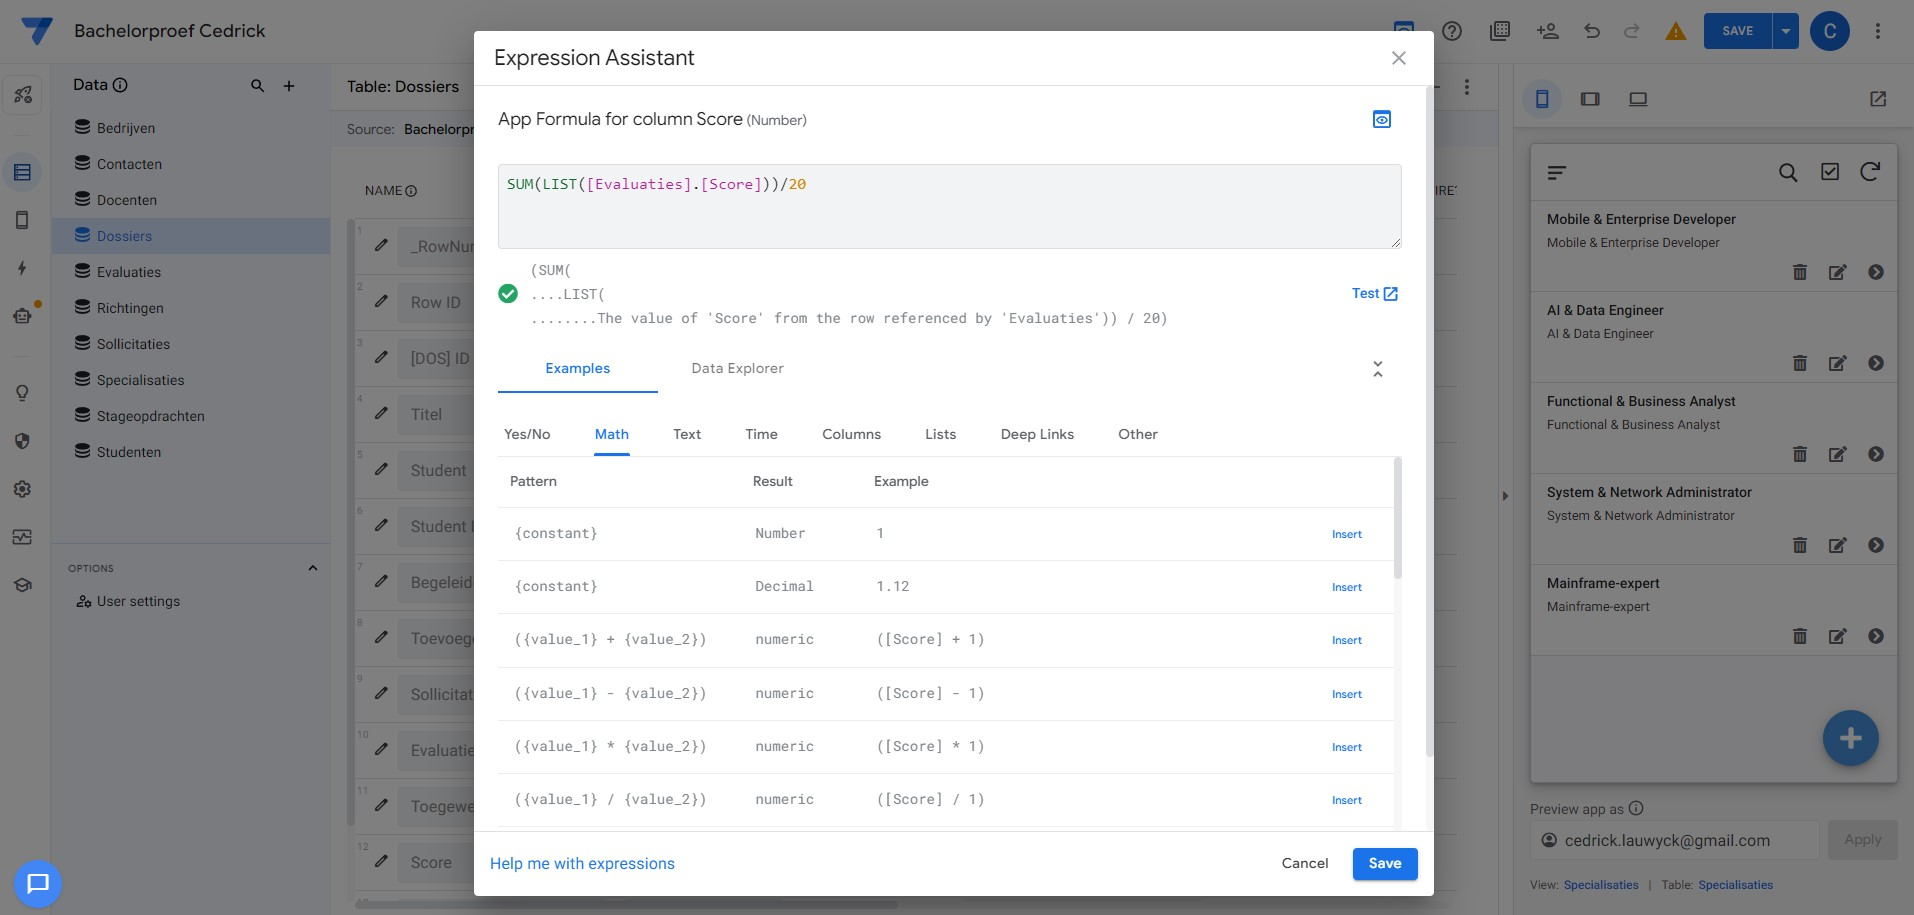
\includegraphics[width=\linewidth]{methodologie/Appsheet_formulaAssistant.jpg}
    \caption{Formules met `Expression Assistant` in Appsheet.}
    \label{fig:meth_appsheet_formulas}
\end{figure}

Een belangrijke opmerking bij Appsheet is dat het aanvullen van de database met gegevens in het applicatiegedeelte gebeurt. Hoewel de mogelijkheid bestaat om rijen toe te voegen in het database gedeelte, zullen op die manier de verschillende formules niet worden toegepast op de data. \\


% automatisaties
Nu kan terug overgegaan worden tot de laatste stap, automatisaties. In Appsheet hoeft enkel de automatisatie voor het omzetten naar pdf-bestand aangemaakt worden. De andere workflows zijn namelijk overbodig, omdat Appsheet al automatisch de mogelijke velden invult indien we op de 'Add'-knop klikken in de applicatie. Automatisaties zijn gemakkelijk te bereiken via een enkele klik op het `robot`-icoontje. Zoals te zien is in figuur \ref{fig:meth_appsheet_automations} wordt een automatisatie in AppSheet gedefinieerd door een zogenaamde `bot`, deze hebben hetzelfde concept als in Podio en Airtable, ze hebben namelijk een set van acties die worden uitgevoerd eens een bepaalde trigger geactiveerd wordt. Voor de use case wordt een bot gezet op de tabel dossiers, met als trigger een verandering in de kolom 'Toevoegen'.
Vervolgens wordt een actie toegevoegd om het dossier om te zetten naar een pdf-bestand. In tegenstelling tot Airtable zit deze functionaliteit net als Podio ingebouwd in AppSheet. Een nadeel is wel dat de gegenereerde pdf achteraf niet zomaar aan het dossier kan worden toegevoegd. Het wordt namelijk opgeslagen op een aparte plaats, zoals Google Drive of OneDrive. Om het bestand te linken aan het dossier, moet een formule worden toegepast op het 'Attachments' veld die verwijst naar de locatie of pad van het pdf-bestand. \\


\begin{figure}[ht]
    \centering
    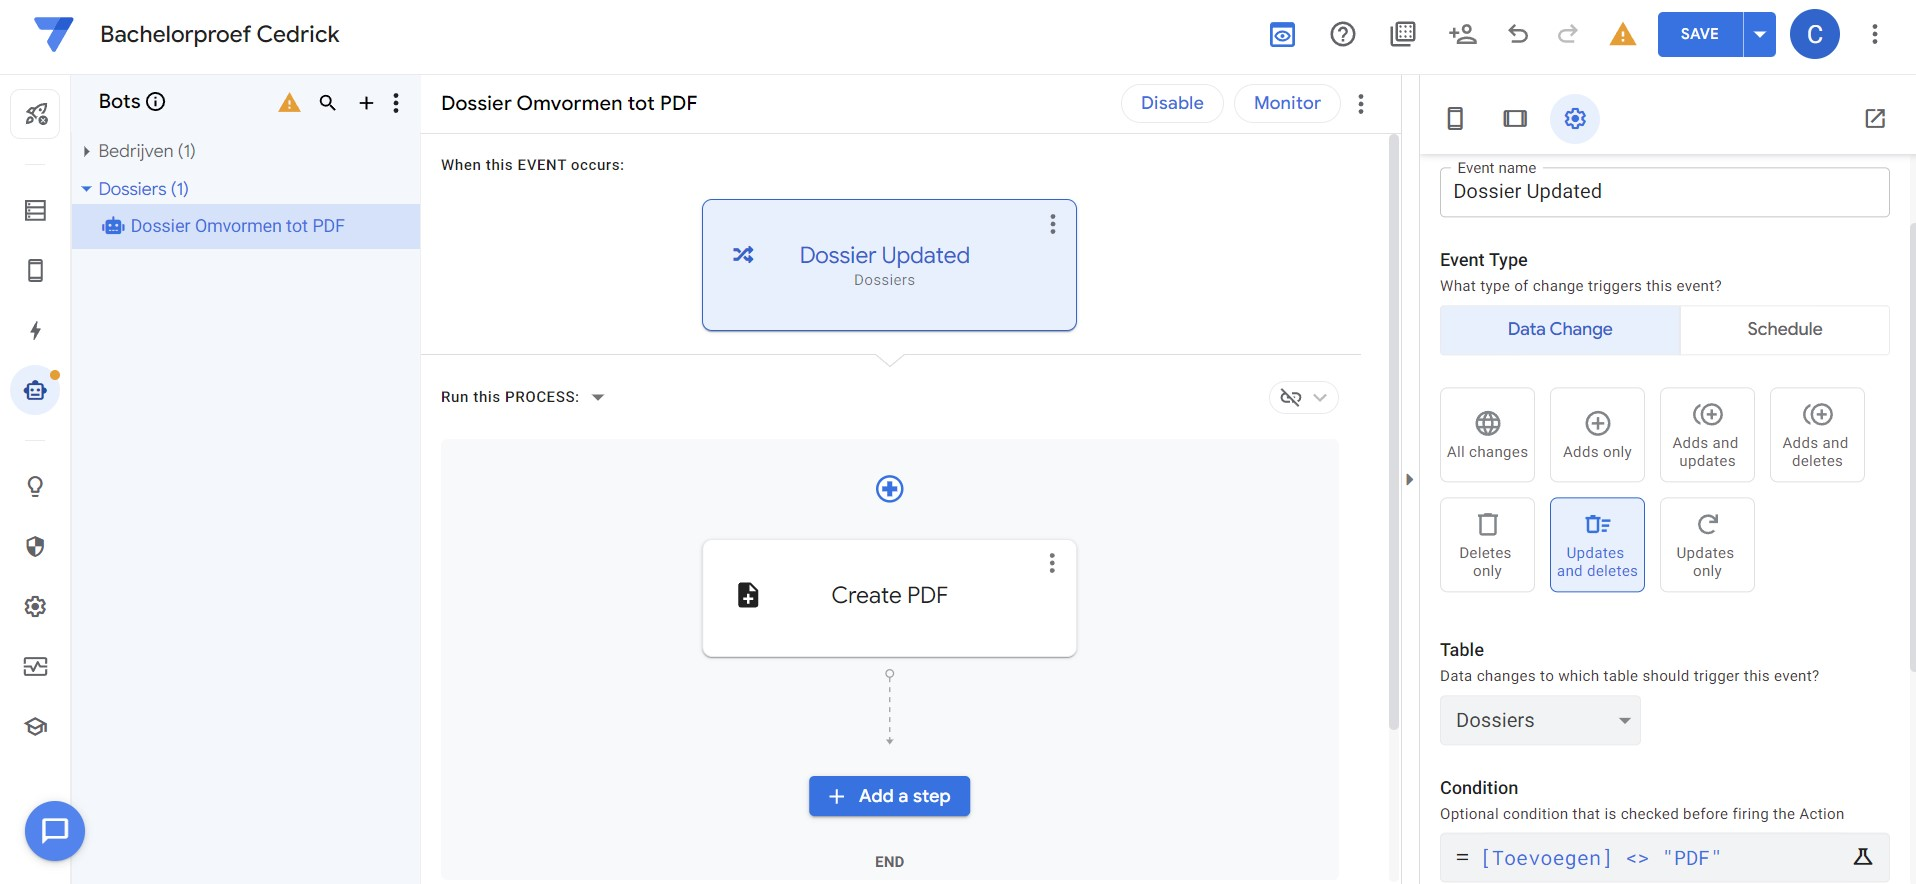
\includegraphics[width=\linewidth]{methodologie/Appsheet_automations.jpg}
    \caption{Automatisaties of 'bots' in Appsheet.}
    \label{fig:meth_appsheet_automations}
\end{figure}


Uiteindelijk is het dus ook perfect mogelijk om de use case uit te bouwen in Appsheet. Net zoals bij Airtable en Podio kunnen er relaties gelegd worden tussen de verschillende tabellen in de database. Verder is het feit dat calculaties op elk veld uitgevoerd kunnen worden een enorm pluspunt, toch is hun functionaliteit beperkter dan de calculatievelden in Podio. Op gebied van gebruikerservaring presteerde Appsheet het minst goed, er waren in het algemeen de meeste klikken\footnote{3 tot 5} en stappen nodig om een doel te bereiken. Daarnaast waren er ook nog extra klikken nodig, zoals het synchroniseren van de database schema's tussen de het applicatie- en databasegedeelte en het heen en weer gaan tussen de 2 delen. Desondanks het feit dat de UI van Appsheet duidelijk opgesteld is, kan ze als onoverzichtelijk overkomen op kleinere schermen, omdat alles dan meer op elkaar gezet wordt en er veel met scrollbars gewerkt moet worden. Ten slotte zijn er ook enkele problemen voorgekomen tijdens het uitwerken van de use case. Vaak waren dit synchronisatie problemen tussen de applicatie en de ingevulde formules. \\


% Voeg hier je eigen hoofdstukken toe die de ``corpus'' van je bachelorproef
% vormen. De structuur en titels hangen af van je eigen onderzoek. Je kan bv.
% elke fase in je onderzoek in een apart hoofdstuk bespreken.

%\input{...}
%\input{...}
%...

%%=============================================================================
%% Conclusie
%%=============================================================================

\chapter{Conclusie}%
\label{ch:conclusie}

% TODO: Trek een duidelijke conclusie, in de vorm van een antwoord op de
% onderzoeksvra(a)g(en). Wat was jouw bijdrage aan het onderzoeksdomein en
% hoe biedt dit meerwaarde aan het vakgebied/doelgroep? 
% Reflecteer kritisch over het resultaat. In Engelse teksten wordt deze sectie
% ``Discussion'' genoemd. Had je deze uitkomst verwacht? Zijn er zaken die nog
% niet duidelijk zijn?
% Heeft het onderzoek geleid tot nieuwe vragen die uitnodigen tot verder 
%onderzoek?

Nu dat het onderzoek uitgevoerd is en de use case succesvol uitgebouwd is in elk platform, kan overgegaan worden tot de conclusie van deze vergelijkende studie. \\

Dit onderzoek biedt een meerwaarde voor Quivvy Solutions BV of andere bedrijven die zich specialiseren in Podio, omdat het weergeeft hoe andere low-code platformen die concurreren met Podio omgaan met eenzelfde use case en hoe dit mogelijks uitgewerkt kan worden. Het geeft ook inzicht in de implementatie van gelijkaardige functionaliteiten zoals workflows en relaties in deze platformen. \\

Verder kan er besloten worden low-code/no-code development platformen in een enorme opmars zijn en dat ze, desondanks de vele uitdagingen, nog een grote impact zullen hebben op de toekomst van development. De mogelijkheid om als non-IT'er toch aan software-ontwikkeling te kunnen doen is duidelijk iets waar steeds meer en meer vraag naar is. \\

Vervolgens is uit het onderzoek gebleken dat AppSheet en Airtable een iets betere implementatie hebben voor het leggen van relaties tussen gegevens. Als het gaat om calculaties, blijft Podio nog steeds veruit het beste platform vanwege de flexibiliteit die het biedt. Podio geeft gebruikers namelijk veel vrijheid om complexe berekeningen en tekstverwerkingen te maken. Verder blinkt Airtable uit op gebied van performantie en gebruikerservaring. Het platform vereist het minste aantal klikken en de pagina's worden zeer snel ingeladen, waardoor gebruikers efficiënt kunnen werken zonder tijd te verspillen aan wachten. Wat betreft automatisaties kunnen de platformen als min of meer gelijkwaardig beschouwd worden, omdat ze bij elk platform zowel voordelen als nadelen hebben ten opzichte van elkaar. Hoewel de platformen verschillen in structuur, blijft de achterliggende werking grotendeels hetzelfde. Ze stellen gebruikers in staat om apps of databases te maken en te beheren, gegevens op te slaan en te organiseren, en aangepaste functionaliteiten toe te voegen aan hun workflows. Kortom, zowel Podio als zijn alternatieven zijn steeds sterke keuzes voor het bouwen van op maat gemaakte low-code software oplossingen. \\

Aangezien er steeds meer low-code platformen uitkomen op de markt is er zeker plaats voor een vervolgonderzoek waar Podio vergeleken kan worden met andere mogelijke alternatieven zoals Notion of Mendix. Daarnaast kan er ook dieper ingegaan worden op specifieke extensies of functionaliteiten binnen Podio. \\ 

Ten slotte kan als antwoord op de algemene onderzoeksvraag van deze studie, namelijk 'Met welke tools kan Quivvy Solutions hetzelfde bereiken als met Podio en hoe geïntegreerd werkt dit?', geconcludeerd worden dat het bedrijf zowel met Airtable als met Google AppSheet dezelfde doeleinden kan bereiken als met Podio, maar dat er wel een nodige inspanning moet gedaan worden om te leren werken met beide alternatieven. Daarnaast kan uit de resultaten van het onderzoek afgeleid worden dat uit de twee alternatieven, Airtable waarschijnlijk een betere keuze is voor het bedrijf dan AppSheet, aangezien het bouwproces probleemloos verliep en het platform de beste gebruikerservaring heeft. \\ 

%---------- Bijlagen -----------------------------------------------------------

\appendix

\chapter{Onderzoeksvoorstel}

Het onderwerp van deze bachelorproef is gebaseerd op een onderzoeksvoorstel dat vooraf werd beoordeeld door de promotor. Dat voorstel is opgenomen in deze bijlage.

% TODO: 
\section*{Samenvatting}

% Kopieer en plak hier de samenvatting (abstract) van je onderzoeksvoorstel.
 Quivvy Solutions BV is een bedrijf dat low-code business oplossingen maakt aan de hand van het Podio platform. Toch zou het bedrijf graag weten of er tegenwoordig een beter alternatief bestaat voor Podio om vervolgens eventueel over te stappen. Om die reden wordt een vergelijkende studie gemaakt tussen Podio, Airtable en Google AppSheet. Dit onderzoek is een verderzetting van een studie van \textcite{Spitaels2022} waarin besloten werd dat Podio beter was dan Airtable op gebied van gebruikerservaring, maar gelijkwaardig op gebied van functionaliteit. In de literatuurstudie worden de alternatieven beschreven en wordt er uitgelegd wat cloud-based management precies is. Als Proof of Concept wordt een use case genomen uit de klantenprojecten van Quivvy Solutions en daarna nagebouwd in Airtable en AppSheet. Aan de hand van deze uitwerking worden de verschillende alternatieven dan vergeleken met Podio op basis van volgende criteria; de verschillen met Podio, de flexibiliteit van het alternatief en de gebruikerservaring. Dit onderzoek zal aantonen hoe deze alternatieven presteren op voorgenoemde criteria en of ze mogelijk een beter alternatief vormen voor Podio.
% Verwijzing naar het bestand met de inhoud van het onderzoeksvoorstel
%---------- Inleiding ---------------------------------------------------------

\section{Introductie}%
\label{sec:introductie}

De afgelopen jaren hebben bedrijven steeds meer nood aan een gecentraliseerde structuur waarin al hun processen samenkomen en opgevolgd kunnen worden. Om die reden werd Podio ontwikkeld, een low-code tool waarmee dit soort cloud based business management platform opgebouwd kan worden. In de laatste jaren is de low-code/no-code markt enorm gestegen in populariteit. Volgens een rapport van Gartner, zou tegen 2024 zelfs meer dan 65\% van de applicaties gemaakt worden in een low-code/no-code omgeving \autocite{Costello2021}.

Quivvy Solutions BV is een bedrijf dat low-code software-oplossingen op maat maakt, met een minimum aan tools en een maximum aan functionaliteit. Hiervoor gebruiken zij Podio, maar ondertussen zijn er al een groot aantal concurrenten, zoals Google AppSheet en Airtable. Kunnen ze met deze tools hetzelfde bereiken als met Podio en hoe geïntegreerd werkt dit? In hoeverre is wat ze met Podio kunnen, ook mogelijk via AirTable en via het Google ecosysteem met Google App Sheets.

%---------- Stand van zaken ---------------------------------------------------

\section{State-of-the-art}%
\label{sec:state-of-the-art}

 Vorig academiejaar werd reeds een vergelijkende studie gemaakt tussen Podio, ClickUp en Airtable door \textcite{Spitaels2022}, dit onderzoek zal deze studie verderzetten. Podio zal vergeleken worden  AppSheet, een no-code development platform. Vervolgens zal op aanvraag van mijn stagebedrijf Airtable verder onderzocht worden, omdat het platform snel evolueert en al heel wat aanpassingen heeft aangebracht.
 
\subsection{Cloud based management}

Een cloud-based management platform wordt door \textcite{Spitaels2022} gedefiniëerd als 'Een tool die er voor gaat zorgen dat een bedrijf vanuit één centrale plek al zijn processen kan bijhouden, uitvoeren en bijsturen en dit terwijl iedereen met dezelfde data te werk gaat en ondertussen snel kan communiceren met elkaar.'
Podio was een voorloper in dit domein.

\subsection{Podio}

Podio is een cloud-based management platform dat gebruikers toelaat om op maat gemaakte business software te ontwikkelen. Het kan alle business processen aggregeren in een enkel platform en kan probleemloos uitgebreid worden naar de wensen van de gebruiker. Het voorziet diverse bouwblokken voor het bouwen van mobiele- en desktop applicaties en automatiseringen. Vervolgens bevat Podio een goede API waardoor het gemakkelijk externe software en tools kan integreren. Om die reden kan het eenvoudig externe applicaties onderhouden vanuit een enkel systeem \autocite{Quivvy}.  


\subsection{Airtable}

Airtable is een flexibele low-code/no-code tool waarmee op maat gemaakte applicaties gebouwd kunnen worden. Het is in staat om processen te visualiseren aan de hand van data uit een interne database. Daarnaast laat het toe om externe tools te integreren zodat taken zoals een email verzenden, kunnen geautomatiseerd worden. Daarbovenop heeft het ook ingebouwde functies waarmee het repetitieve taken kan automatiseren. Zo hoeft de gebruiker hieraan geen tijd te besteden en kan ze de focus leggen op zaken die belangrijker zijn \autocite{Airtable}.

\subsection{AppSheet}

AppSheet is een no-code development platform dat werd overgenomen door Google in 2020. Het laat toe om mobiele en desktop applicaties te bouwen zonder code te hoeven schrijven. Daarnaast is het in staat om bots aan te maken die taken zoals emails verzenden gaan automatiseren. Vervolgens is er ook de mogelijkheid om externe applicaties zoals SQL databases te integreren \autocite{AppSheet2020}. 


%---------- Methodologie ------------------------------------------------------
\section{Methodologie}%
\label{sec:methodologie}

Het onderzoek zal verlopen op basis van een lijst vergelijkingscriteria die door mijn stagebedrijf werd voorzien. 

\begin{itemize}
    \item Ten eerste zal nagegaan worden of het alternatief past bij het doel, namelijk low code business software die op maat gemaakt is voor diverse bedrijfscontexten. Hoeveel code is er nodig om dit te bereiken en hoe eenvoudig is het om alles vanuit één plaats te beheren?
    \item Ten tweede wordt onderzocht hoe flexibel het alternatief is. Zijn er eventuele beperkingen? Hoe gemakkelijk kunnen processen aangepast worden?
    \item Ten derde wordt gekeken in hoeverre de kernelementen van Podio aanwezig zijn in het alternatief. Is er een relationele database met de mogelijkheid om alles met elkaar te linken?  Zijn er calculatievelden om berekeningen uit te voeren of om dynamisch tekst te tonen? Is het alternatief in staat om automatiseringen uit te voeren? Kan het integreren met andere tools via API-connecties?
    \item Ten slotte wordt de gebruikerservaring onderzocht, hoe clean is de gebruikersinterface en hoe gemakkelijk is die te gebruiken? Hoeveel clicks, vensters, $\ldots$ zijn er om een bepaalde actie uit te voeren?
\end{itemize}

De vergelijkende studie zal antwoord bieden op volgende onderzoeksvragen:

\begin{itemize}
    \item Welke verschillen zijn er tussen Podio en zijn alternatieven?
    \item Op welke gebieden presteren de alternatieven beter of slechter dan Podio?
    \item Is de overstap van Podio naar een nieuwer alternatief de nodige inspanning waard?
\end{itemize}

%---------- Verwachte resultaten ----------------------------------------------
\section{Verwacht resultaat, conclusie}%
\label{sec:verwachte_resultaten}

Er wordt verwacht dat Podio goede resultaten zal behalen, omdat het een voorloper is en een zeer groot aanbod aan features heeft. Vervolgens wordt er verwacht dat Airtable minstens even sterk zal presteren als Podio. In het onderzoek van \textcite{Spitaels2022} werd geconcludeerd dat het een gelijkwaardig platform is aan Podio op gebied van functionaliteiten, maar dat het wel slechter presteerde op gebied van gebruikerservaring. Om die reden wordt er verwacht dat Airtable enige inspanningen gedaan heeft om zijn gebruikerservaring te verbeteren. Ten laatste wordt er verwacht dat AppSheet ook hoge resultaten zal halen, omdat het eigendom is van gigant Google en gebruik kan maken van Google's grote aantal resources.

De resultaten van het onderzoek kunnen een meerwaarde vormen voor mijn stagebedrijf. Ze werken dagelijks met Podio en willen steeds op de hoogte zijn van andere opkomende tools.



%%---------- Andere bijlagen --------------------------------------------------
% TODO: Voeg hier eventuele andere bijlagen toe. Bv. als je deze BP voor de
% tweede keer indient, een overzicht van de verbeteringen t.o.v. het origineel.
%\input{...}

%%---------- Backmatter, referentielijst ---------------------------------------

\backmatter{}

\setlength\bibitemsep{2pt} %% Add Some space between the bibliograpy entries
\printbibliography[heading=bibintoc]

\end{document}
